% Options for packages loaded elsewhere
\PassOptionsToPackage{unicode}{hyperref}
\PassOptionsToPackage{hyphens}{url}
%
\documentclass[
  9pt,
]{book}
\usepackage[]{mathpazo}
\usepackage{amssymb,amsmath}
\usepackage{ifxetex,ifluatex}
\ifnum 0\ifxetex 1\fi\ifluatex 1\fi=0 % if pdftex
  \usepackage[T1]{fontenc}
  \usepackage[utf8]{inputenc}
  \usepackage{textcomp} % provide euro and other symbols
\else % if luatex or xetex
  \usepackage{unicode-math}
  \defaultfontfeatures{Scale=MatchLowercase}
  \defaultfontfeatures[\rmfamily]{Ligatures=TeX,Scale=1}
\fi
% Use upquote if available, for straight quotes in verbatim environments
\IfFileExists{upquote.sty}{\usepackage{upquote}}{}
\IfFileExists{microtype.sty}{% use microtype if available
  \usepackage[]{microtype}
  \UseMicrotypeSet[protrusion]{basicmath} % disable protrusion for tt fonts
}{}
\makeatletter
\@ifundefined{KOMAClassName}{% if non-KOMA class
  \IfFileExists{parskip.sty}{%
    \usepackage{parskip}
  }{% else
    \setlength{\parindent}{0pt}
    \setlength{\parskip}{6pt plus 2pt minus 1pt}}
}{% if KOMA class
  \KOMAoptions{parskip=half}}
\makeatother
\usepackage{xcolor}
\IfFileExists{xurl.sty}{\usepackage{xurl}}{} % add URL line breaks if available
\IfFileExists{bookmark.sty}{\usepackage{bookmark}}{\usepackage{hyperref}}
\hypersetup{
  pdftitle={Supplement to Longitudinal analysis of child wasting and concurrence with stunting in low-resource settings},
  pdfauthor={Andrew Mertens et al.},
  hidelinks,
  pdfcreator={LaTeX via pandoc}}
\urlstyle{same} % disable monospaced font for URLs
\usepackage{longtable,booktabs}
% Correct order of tables after \paragraph or \subparagraph
\usepackage{etoolbox}
\makeatletter
\patchcmd\longtable{\par}{\if@noskipsec\mbox{}\fi\par}{}{}
\makeatother
% Allow footnotes in longtable head/foot
\IfFileExists{footnotehyper.sty}{\usepackage{footnotehyper}}{\usepackage{footnote}}
\makesavenoteenv{longtable}
\usepackage{graphicx,grffile}
\makeatletter
\def\maxwidth{\ifdim\Gin@nat@width>\linewidth\linewidth\else\Gin@nat@width\fi}
\def\maxheight{\ifdim\Gin@nat@height>\textheight\textheight\else\Gin@nat@height\fi}
\makeatother
% Scale images if necessary, so that they will not overflow the page
% margins by default, and it is still possible to overwrite the defaults
% using explicit options in \includegraphics[width, height, ...]{}
\setkeys{Gin}{width=\maxwidth,height=\maxheight,keepaspectratio}
% Set default figure placement to htbp
\makeatletter
\def\fps@figure{htbp}
\makeatother
\setlength{\emergencystretch}{3em} % prevent overfull lines
\providecommand{\tightlist}{%
  \setlength{\itemsep}{0pt}\setlength{\parskip}{0pt}}
\setcounter{secnumdepth}{5}
\usepackage{booktabs}
\usepackage{amsthm}
\makeatletter
\def\thm@space@setup{%
  \thm@preskip=8pt plus 2pt minus 4pt
  \thm@postskip=\thm@preskip
}
\makeatother
\usepackage[]{natbib}
\bibliographystyle{apalike}

\title{Supplement to Longitudinal analysis of child wasting and concurrence with stunting in low-resource settings}
\author{Andrew Mertens et al.}
\date{2020-06-10}

\begin{document}
\maketitle

{
\setcounter{tocdepth}{1}
\tableofcontents
}
\hypertarget{overview}{%
\chapter{Overview}\label{overview}}

\textbf{Recommended citation:} Mertens A N, et al.~2020. Longitudinal analysis of child wasting and concurrence with stunting in low-resource settings. \emph{Journal Name}. doi.

This site contains supplementary information to the \emph{Longitudinal analysis of child wasting and concurrence with stunting in low-resource settings}.

\hypertarget{fixed-effects}{%
\chapter{Sensitivity analysis using fixed effects}\label{fixed-effects}}

\raggedright

The primary analyses presented in this manuscript pooled across individual studies using random effects. Inferences about estimates from fixed effects models are restricted to only the included studies.\footnote{Hedges, L. V. \& Vevea, J. L. Fixed- and random-effects models in meta-analysis. Psychol. Methods 3, 486--504 (1998).} The random effects approach is more conservative in the presence of study heterogeneity and has larger confidence intervals around each point estimate unless all cohort-specific estimates are very similiar. Overall, the inference from results produced by each method did not greatly differ.

\hypertarget{age-specific-prevalence}{%
\section{Age-specific prevalence}\label{age-specific-prevalence}}

\hypertarget{random-effects}{%
\subsection{Random effects}\label{random-effects}}

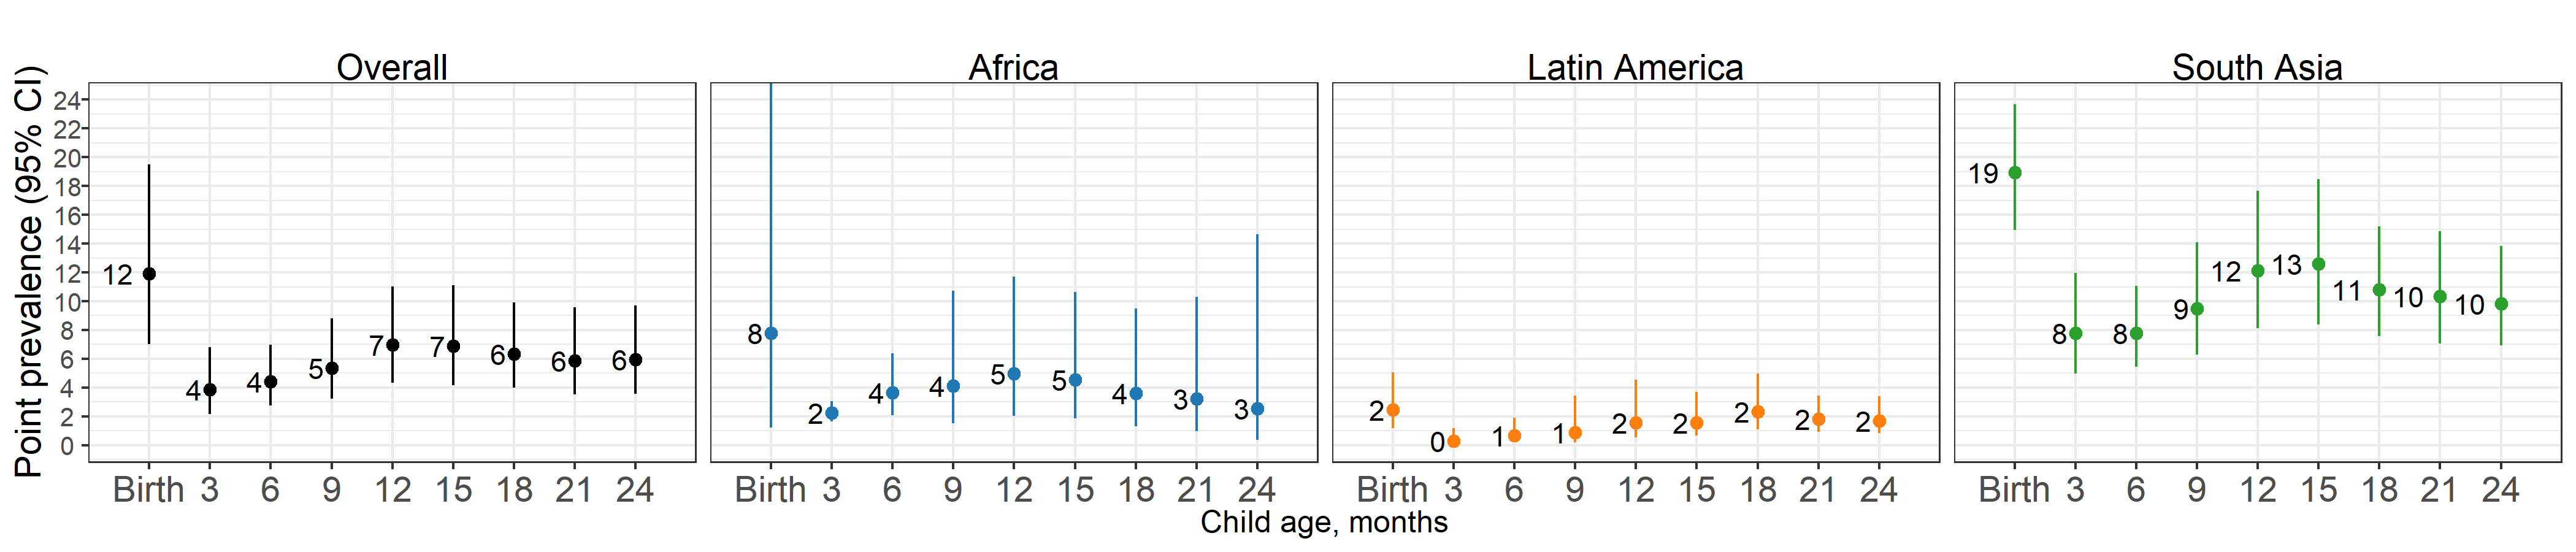
\includegraphics[width=58.33in]{C:/Users/andre/Documents/HBGDki/wasting/ki-longitudinal-manuscripts/figures/wasting/fig-wast-2-prev-overall_region--allage-primary}

\hypertarget{fixed-effects-1}{%
\subsection{Fixed effects}\label{fixed-effects-1}}

\hypertarget{age-specific-incidence}{%
\section{Age-specific incidence}\label{age-specific-incidence}}

\hypertarget{random-effects-1}{%
\subsection{Random effects}\label{random-effects-1}}

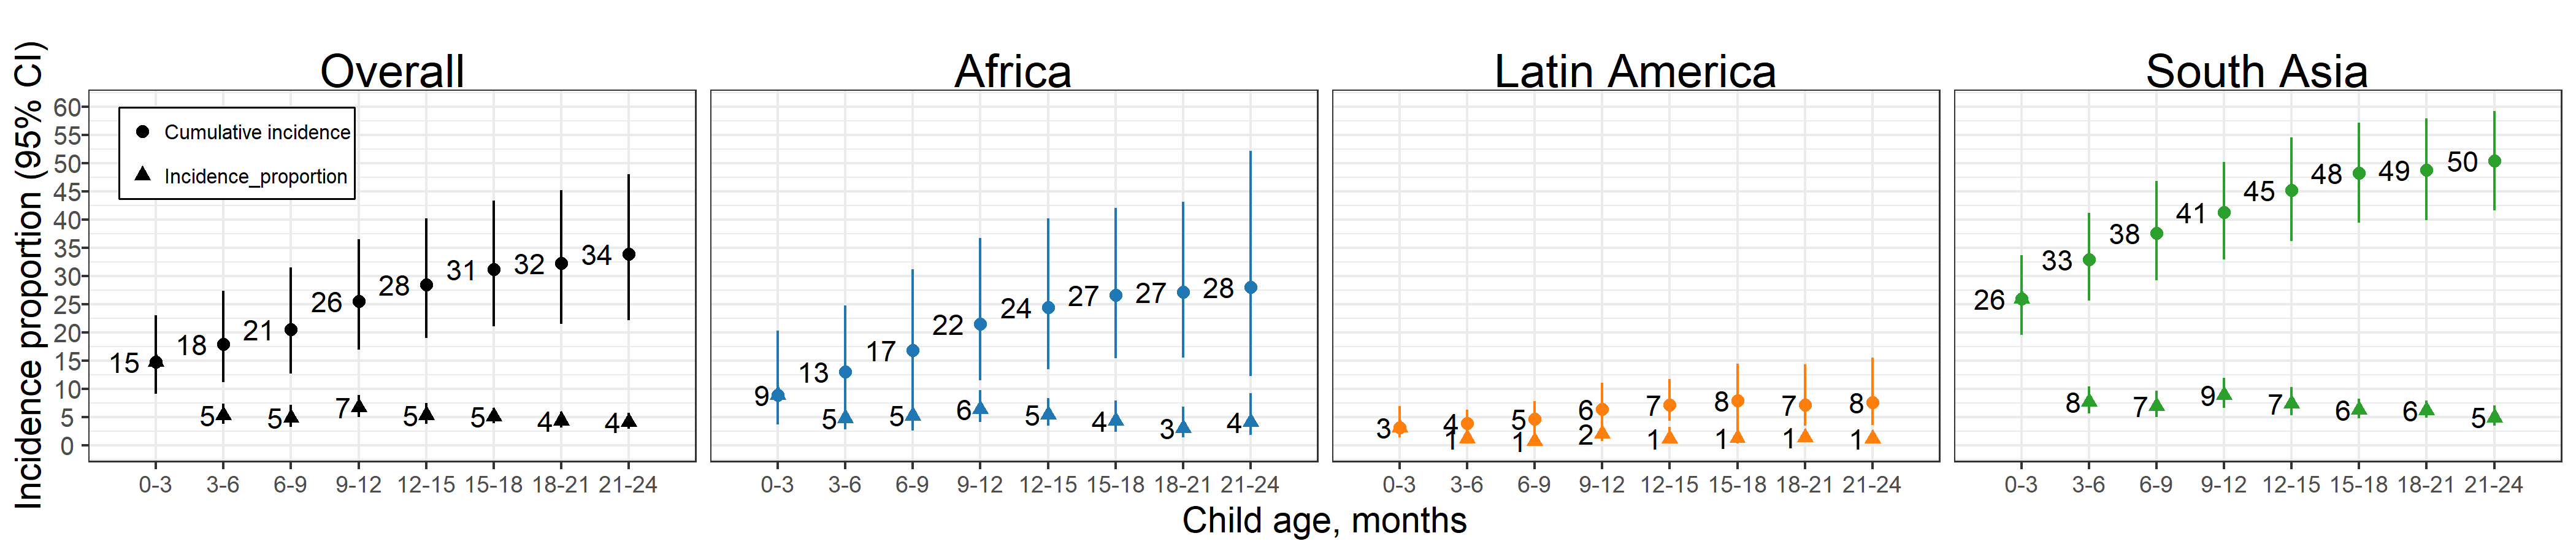
\includegraphics[width=58.33in]{C:/Users/andre/Documents/HBGDki/wasting/ki-longitudinal-manuscripts/figures/wasting/fig-wast-2-cuminc-overall_region--allage-primary}

\hypertarget{fixed-effects-2}{%
\subsection{Fixed effects}\label{fixed-effects-2}}

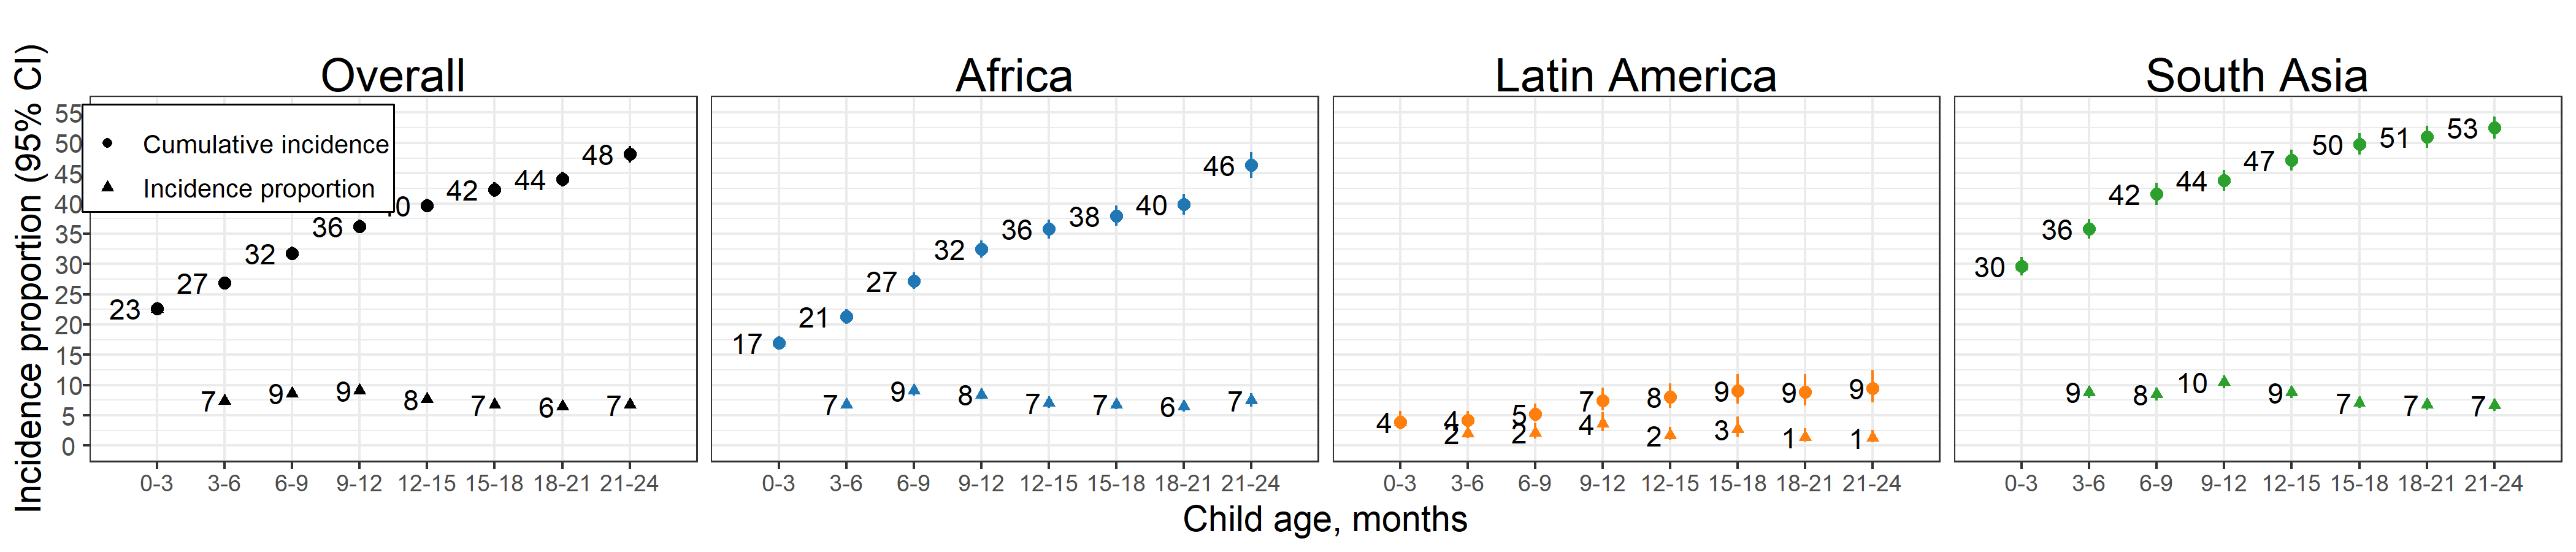
\includegraphics[width=58.33in]{C:/Users/andre/Documents/HBGDki/wasting/ki-longitudinal-manuscripts/figures/wasting/FE/fig-wast-2-cuminc-overall_region--allage-primary_FE}

\hypertarget{age-specific-incidence-rate}{%
\section{Age-specific incidence rate}\label{age-specific-incidence-rate}}

\hypertarget{random-effects-2}{%
\subsection{Random effects}\label{random-effects-2}}

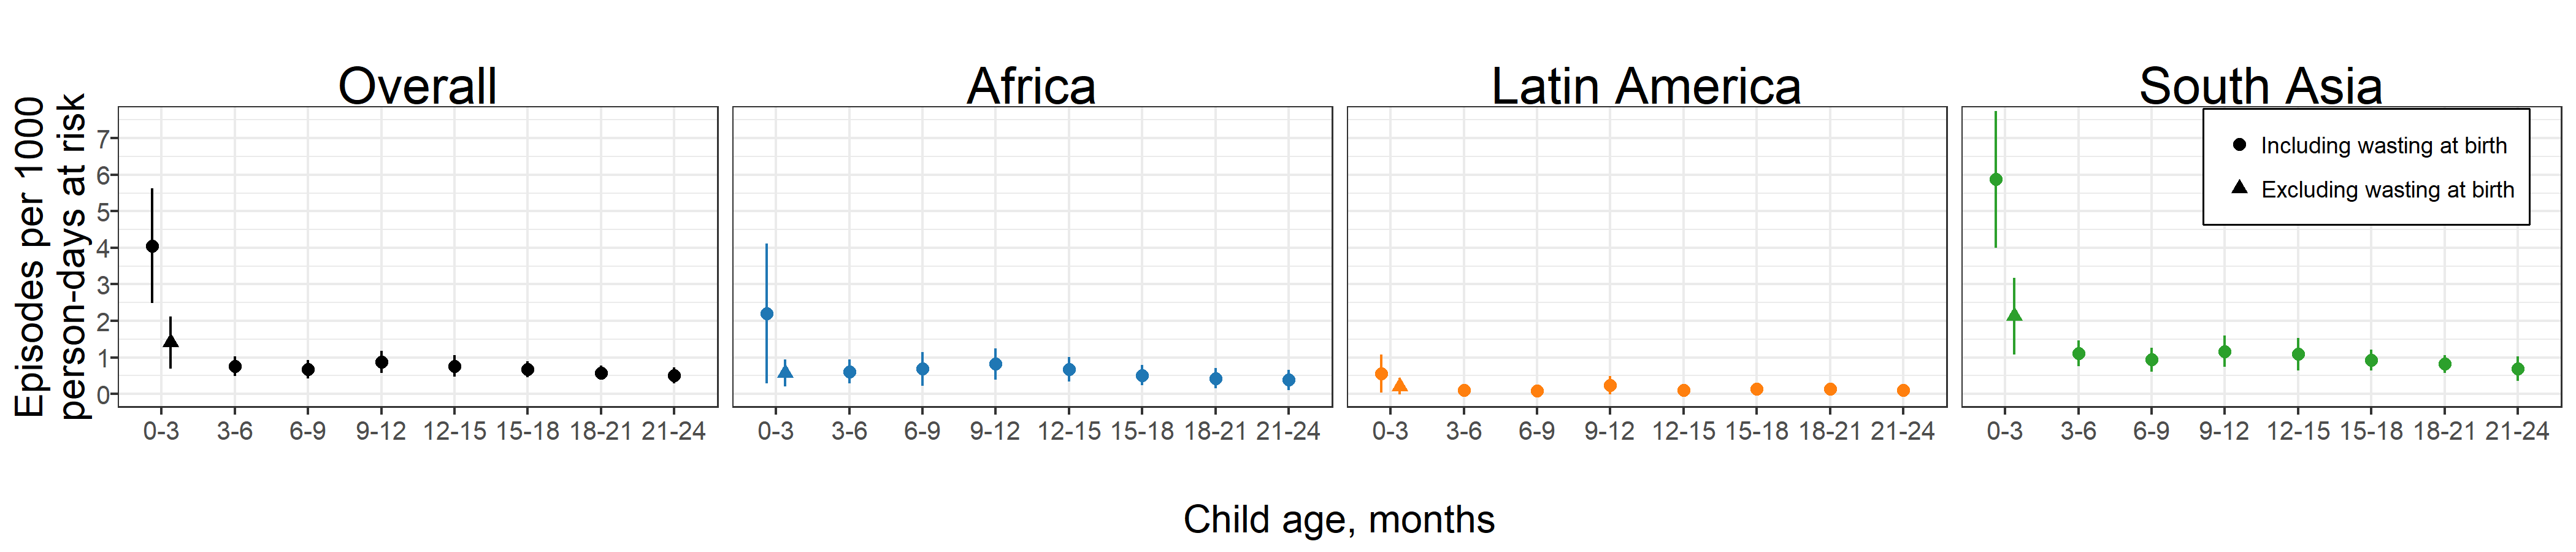
\includegraphics[width=58.33in]{C:/Users/andre/Documents/HBGDki/wasting/ki-longitudinal-manuscripts/figures/wasting/fig-wast-2-ir-overall_region--allage-primary}

\hypertarget{fixed-effects-3}{%
\subsection{Fixed effects}\label{fixed-effects-3}}

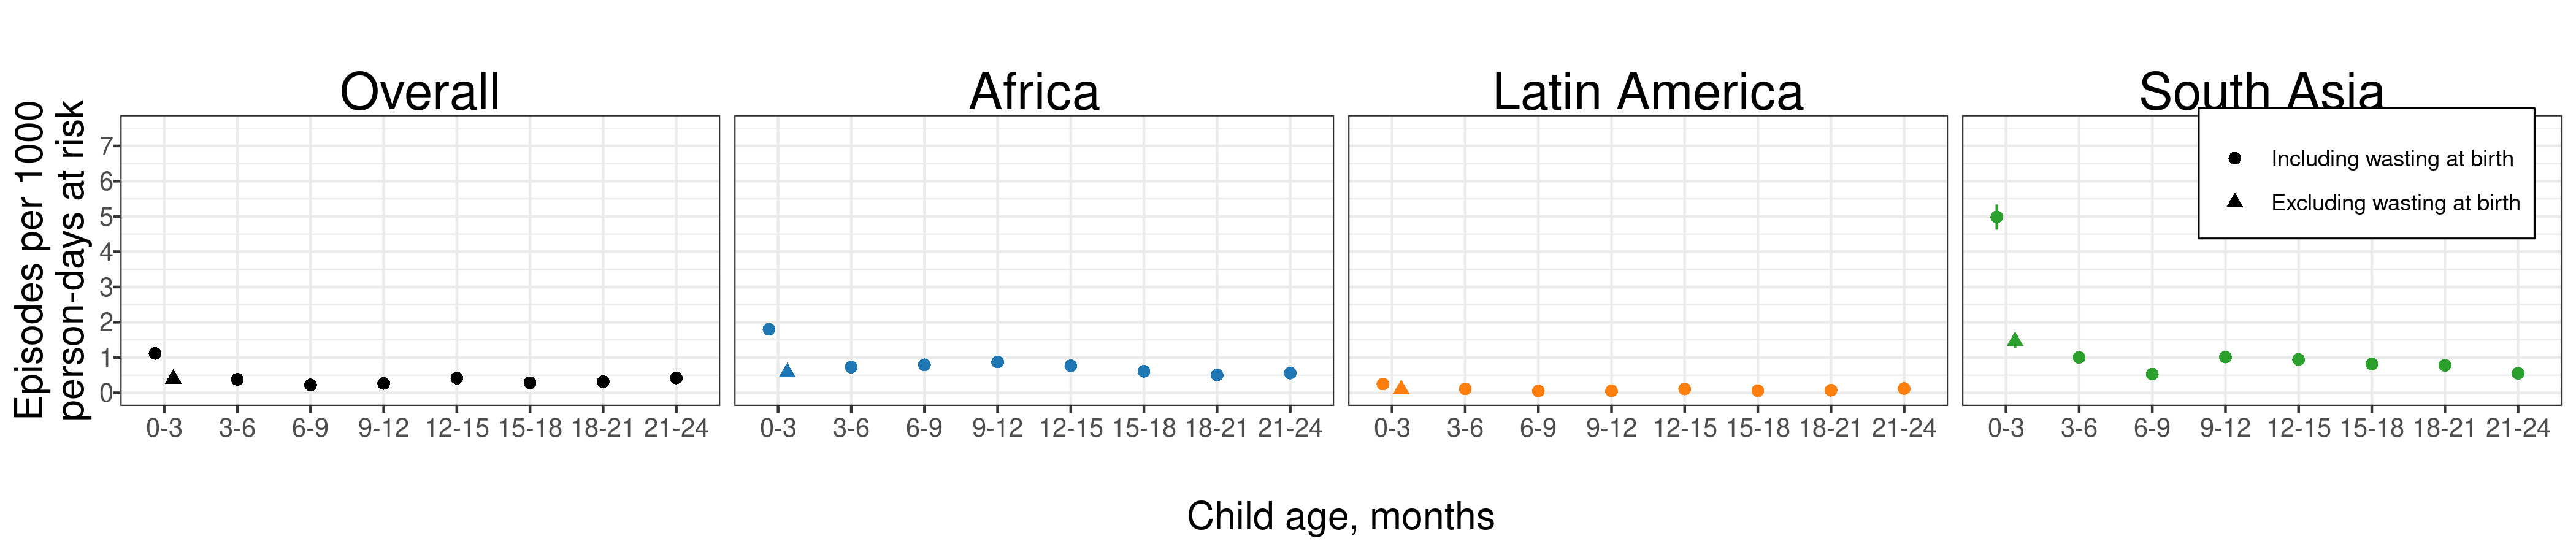
\includegraphics[width=58.33in]{C:/Users/andre/Documents/HBGDki/wasting/ki-longitudinal-manuscripts/figures/wasting/FE/fig-wast-2-ir-overall_region--allage-primary_FE}

\hypertarget{age-specific-recovery}{%
\section{Age-specific recovery}\label{age-specific-recovery}}

\hypertarget{random-effects-3}{%
\subsection{Random effects}\label{random-effects-3}}

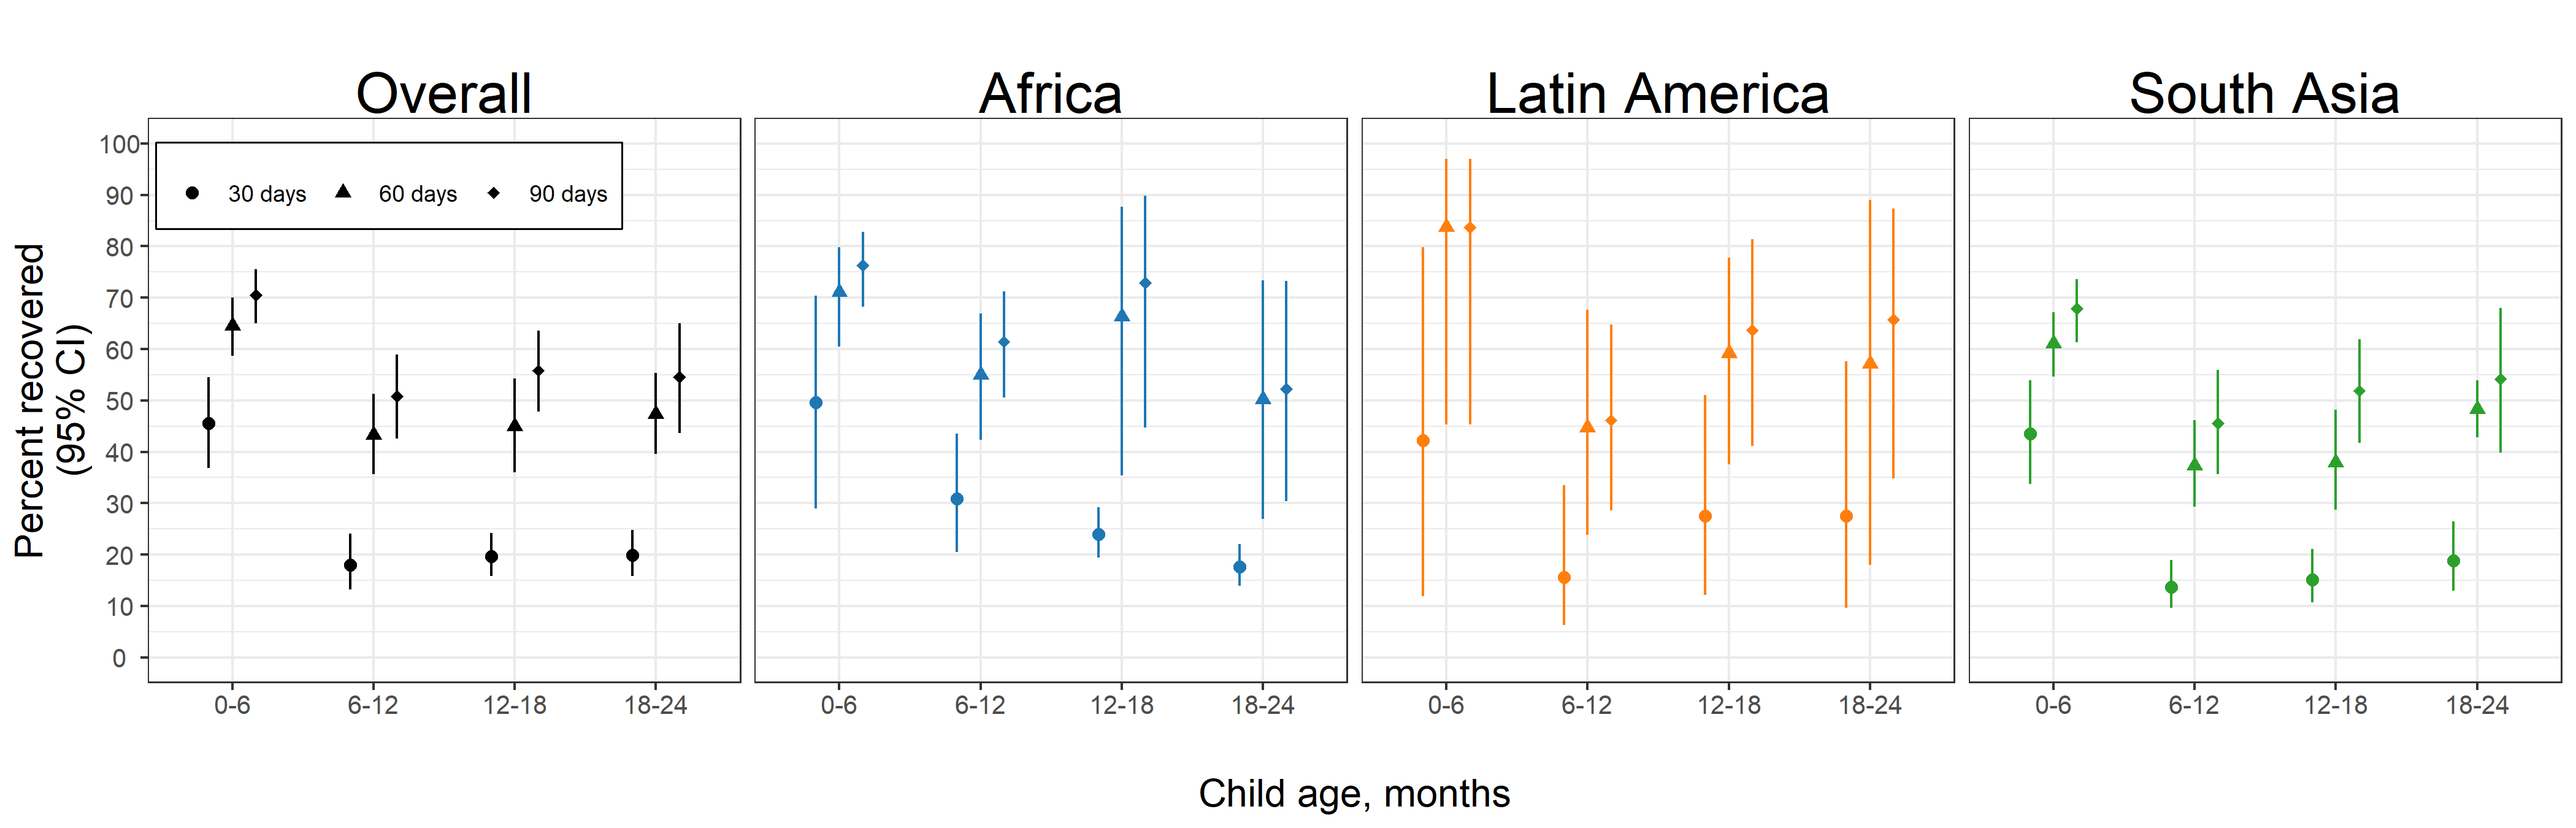
\includegraphics[width=58.33in]{C:/Users/andre/Documents/HBGDki/wasting/ki-longitudinal-manuscripts/figures/wasting/fig-wast-2-rec-overall_region--allage-primary}

\hypertarget{fixed-effects-4}{%
\subsection{Fixed effects}\label{fixed-effects-4}}

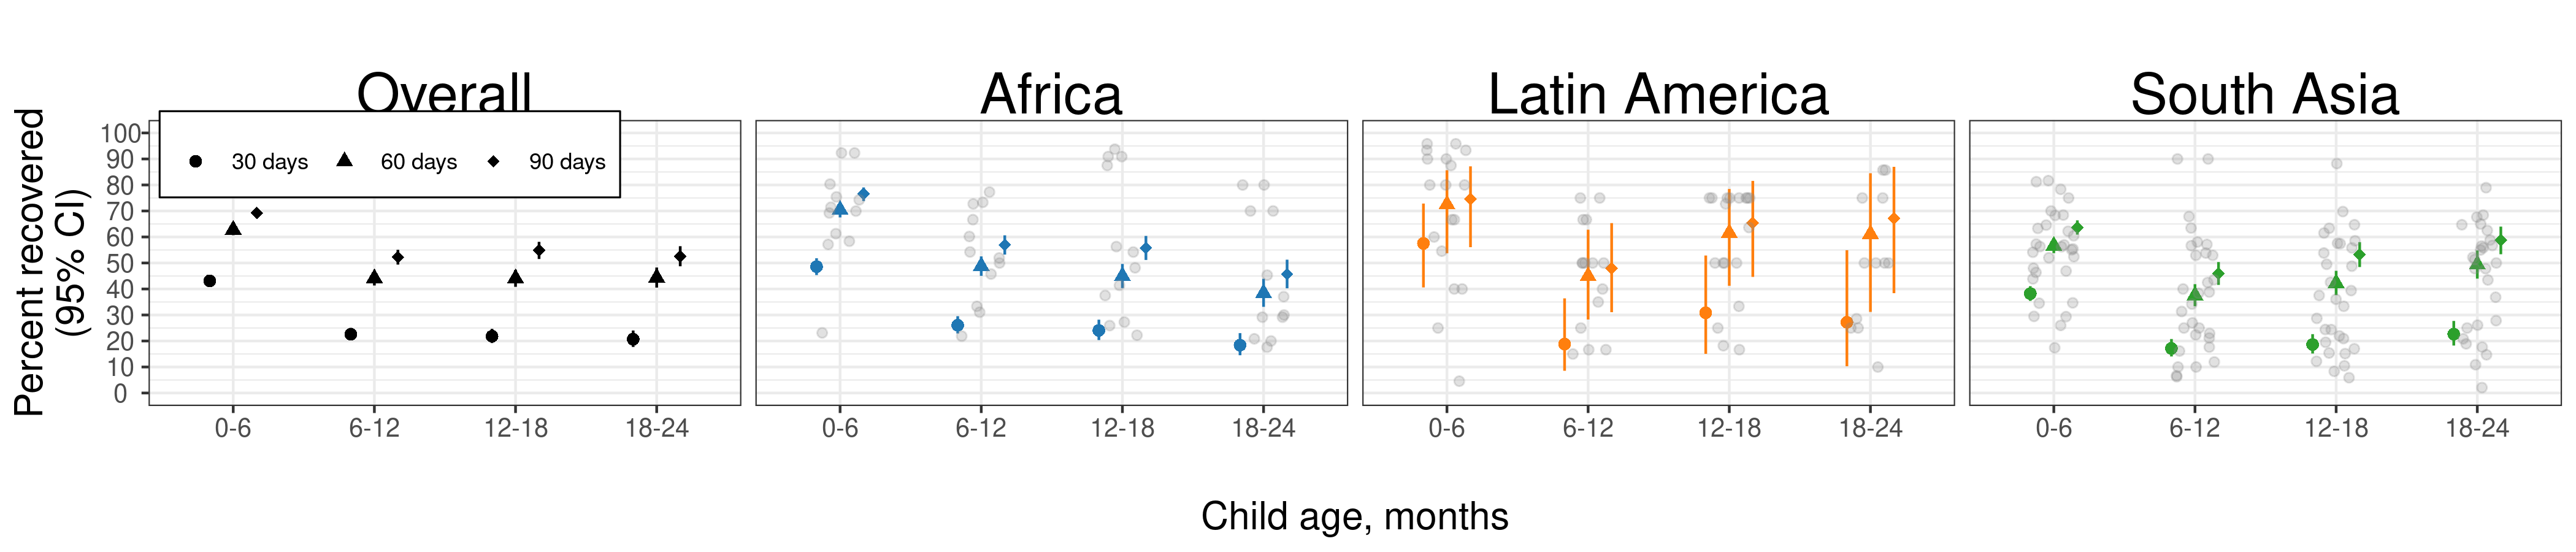
\includegraphics[width=58.33in]{C:/Users/andre/Documents/HBGDki/wasting/ki-longitudinal-manuscripts/figures/wasting/FE/fig-wast-2-rec-overall_region--allage-primary_FE}

\hypertarget{age-specific-prevalence-of-severe-wasting}{%
\section{Age-specific prevalence of severe wasting}\label{age-specific-prevalence-of-severe-wasting}}

\hypertarget{random-effects-4}{%
\subsection{Random effects}\label{random-effects-4}}

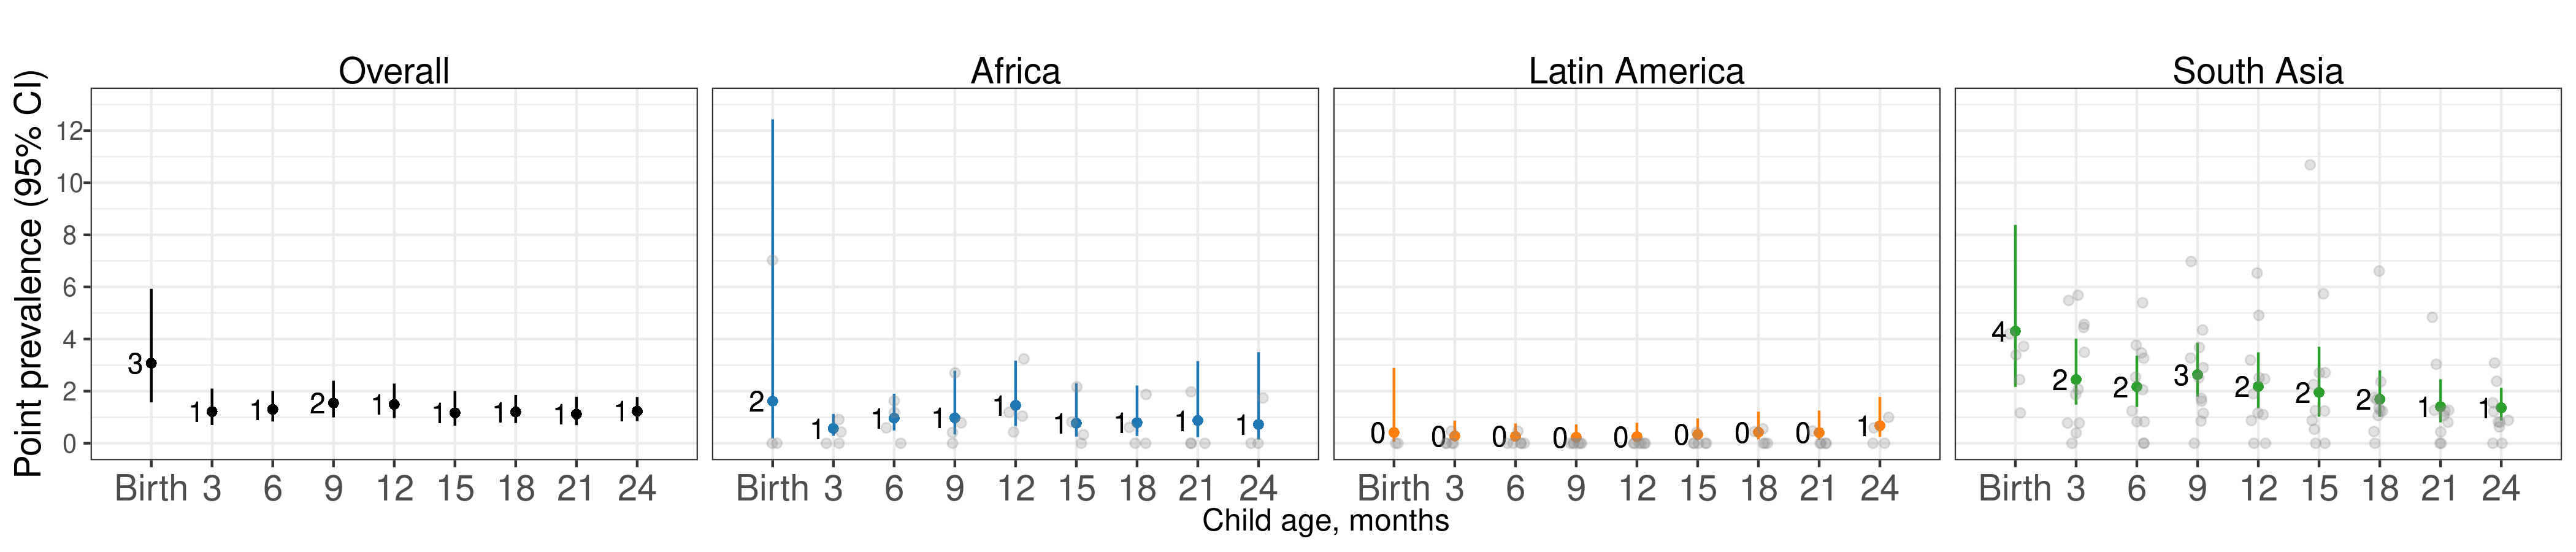
\includegraphics[width=58.33in]{C:/Users/andre/Documents/HBGDki/wasting/ki-longitudinal-manuscripts/figures/wasting/fig-wast-3-prev-overall_region--allage-primary}

\hypertarget{fixed-effects-5}{%
\subsection{Fixed effects}\label{fixed-effects-5}}

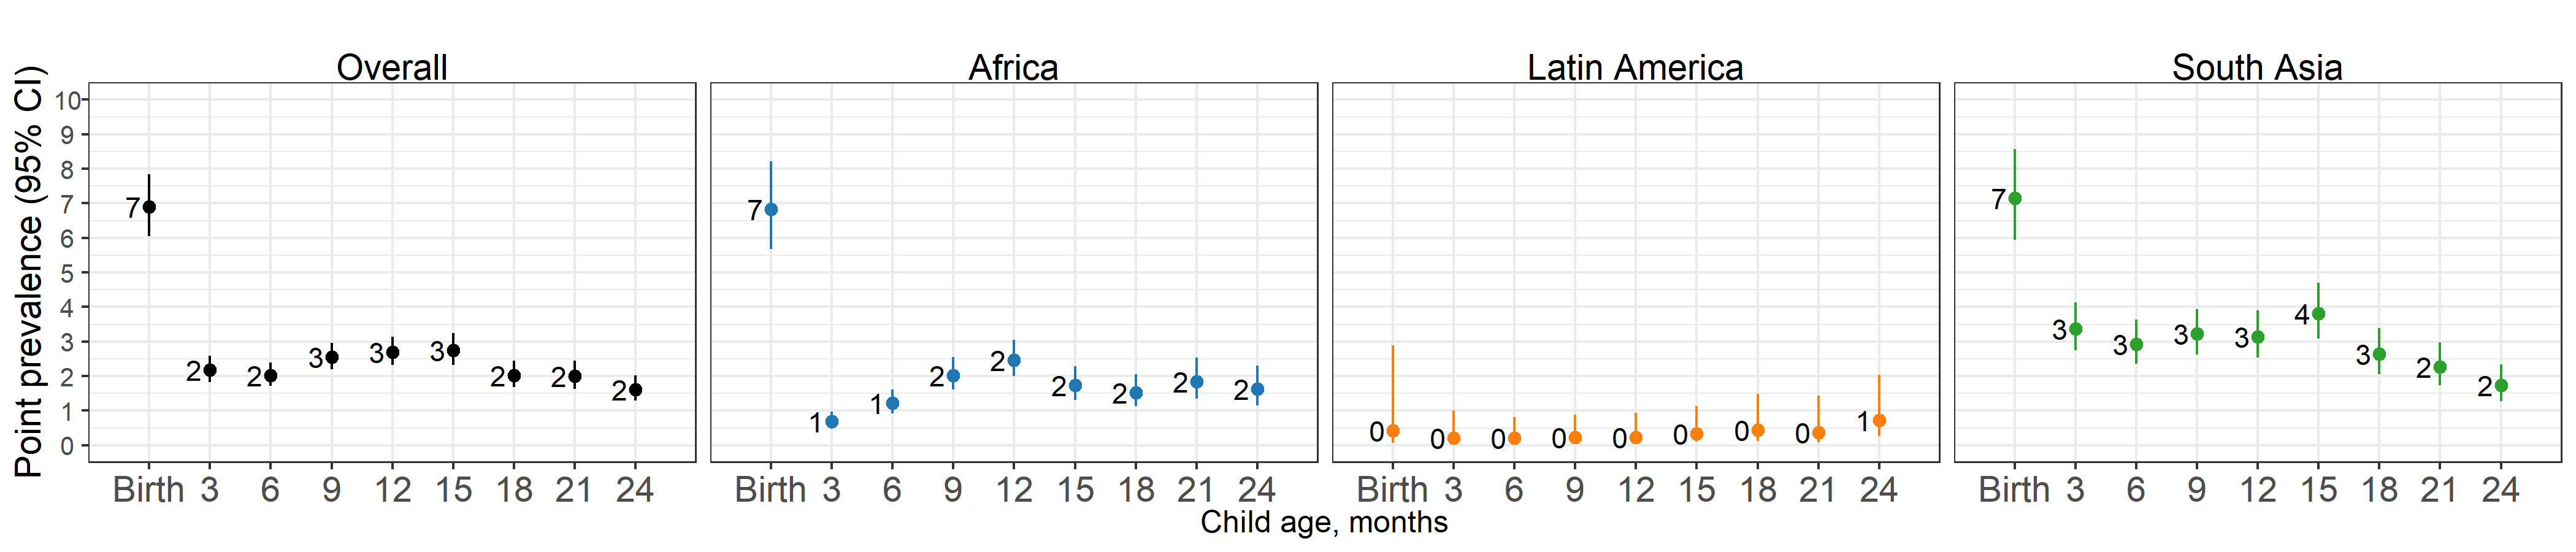
\includegraphics[width=58.33in]{C:/Users/andre/Documents/HBGDki/wasting/ki-longitudinal-manuscripts/figures/wasting/FE/fig-wast-3-prev-overall_region--allage-primary_FE}

\hypertarget{age-specific-longitudinal-prevalence-of-persistent-wasting}{%
\section{Age-specific longitudinal prevalence of persistent wasting}\label{age-specific-longitudinal-prevalence-of-persistent-wasting}}

\hypertarget{random-effects-5}{%
\subsection{Random effects}\label{random-effects-5}}

\hypertarget{fixed-effects-6}{%
\subsection{Fixed effects}\label{fixed-effects-6}}

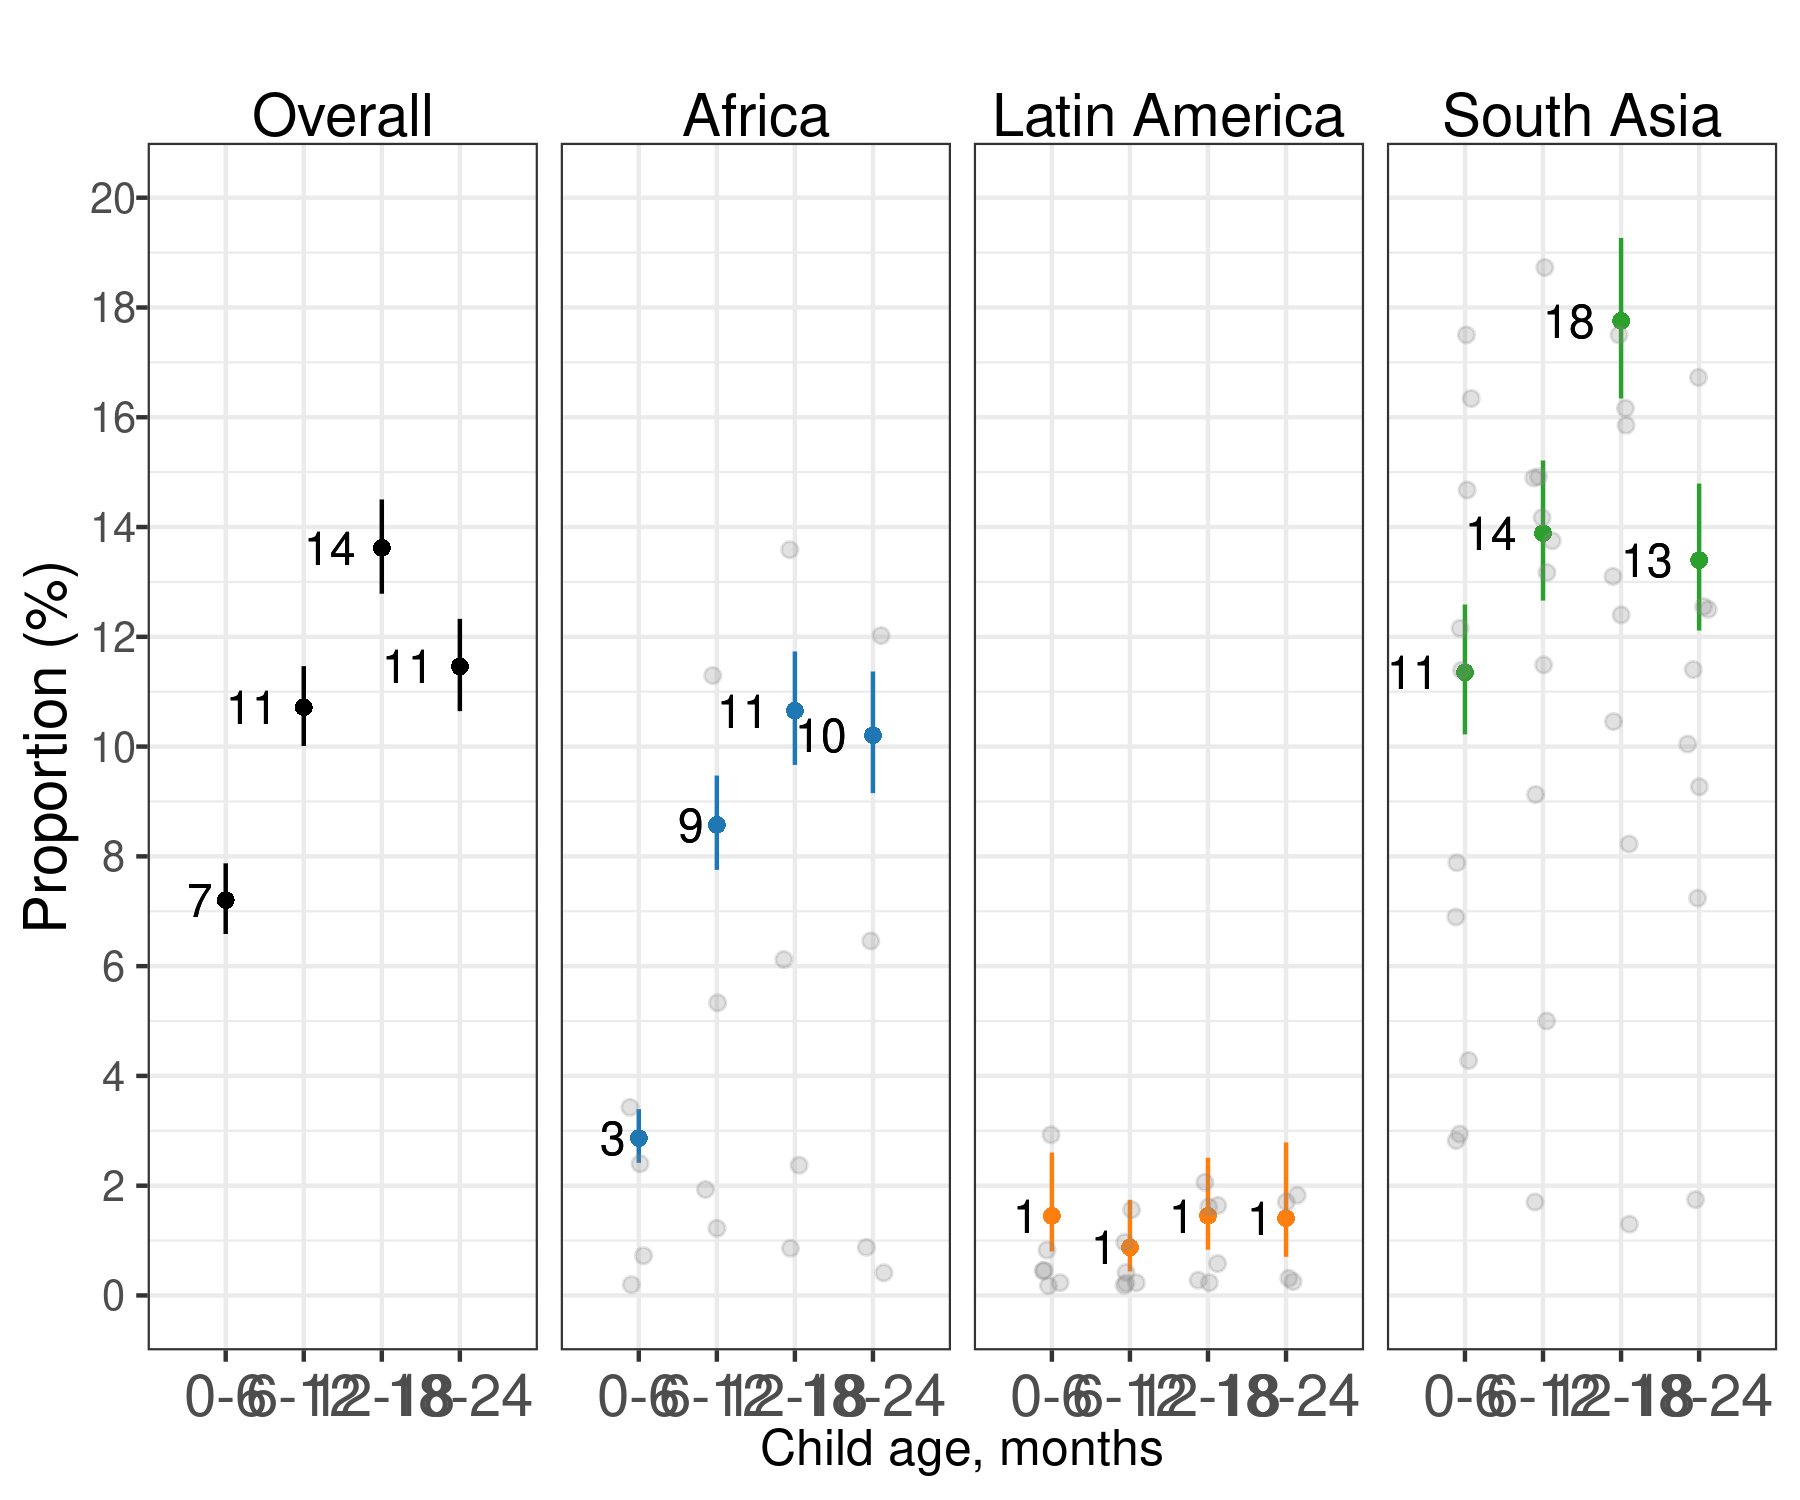
\includegraphics[width=25in]{C:/Users/andre/Documents/HBGDki/wasting/ki-longitudinal-manuscripts/figures/wasting/FE/fig-perswast_plot_FE}

\hypertarget{age-specific-prevalence-of-concurrent-wasting-and-stunting}{%
\section{Age-specific prevalence of concurrent wasting and stunting}\label{age-specific-prevalence-of-concurrent-wasting-and-stunting}}

\hypertarget{random-effects-6}{%
\subsection{Random effects}\label{random-effects-6}}

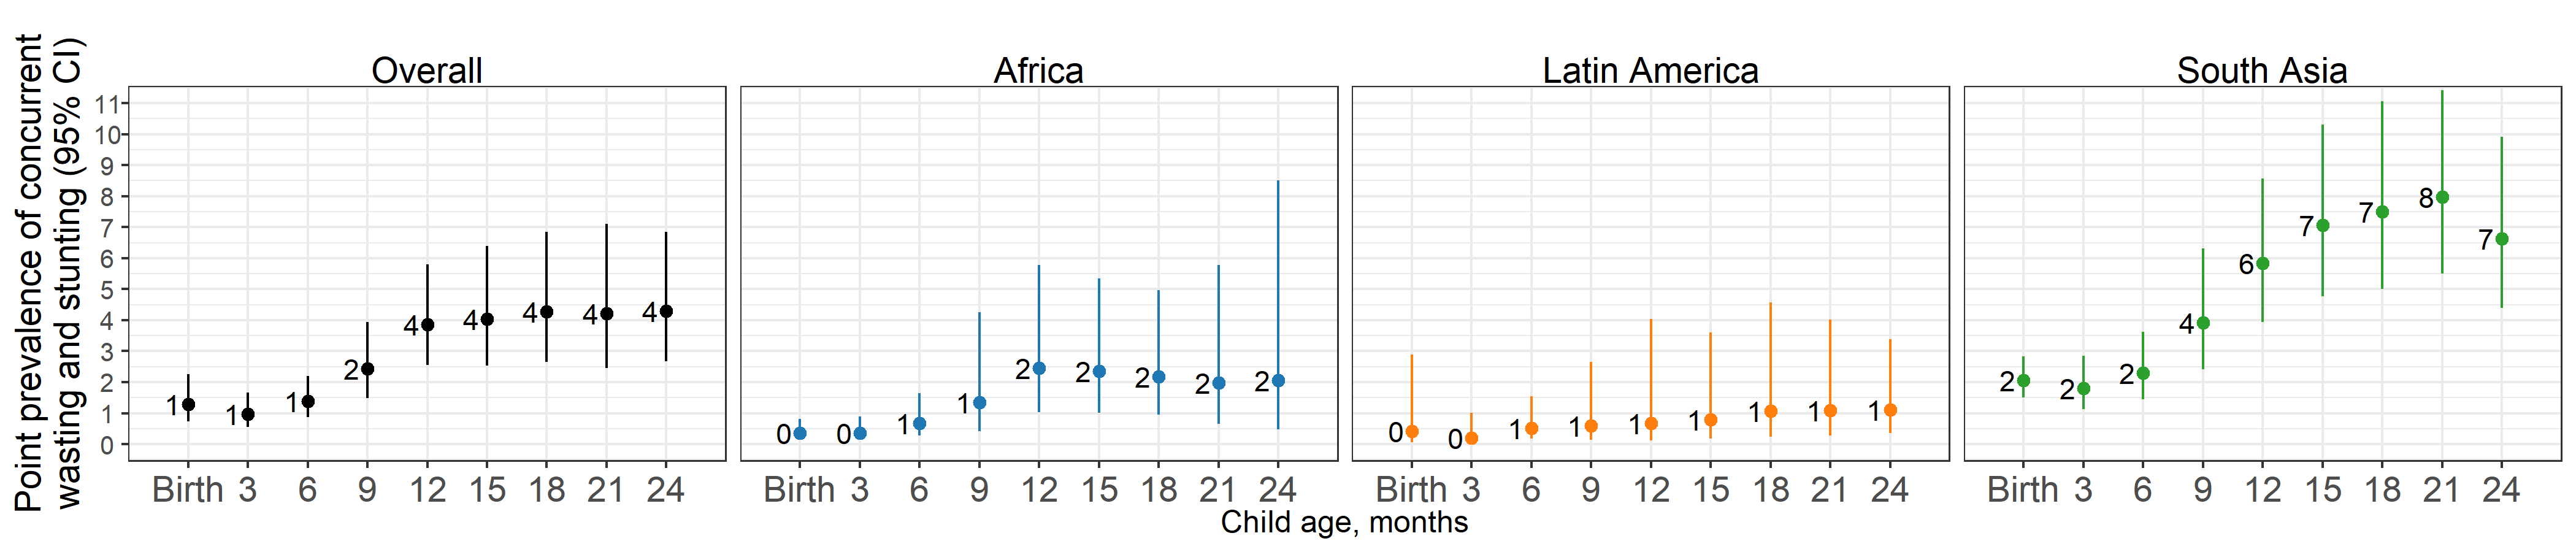
\includegraphics[width=58.33in]{C:/Users/andre/Documents/HBGDki/wasting/ki-longitudinal-manuscripts/figures/wasting/fig-wast-2-co-overall_region--allage-primary}

\hypertarget{fixed-effects-7}{%
\subsection{Fixed effects}\label{fixed-effects-7}}

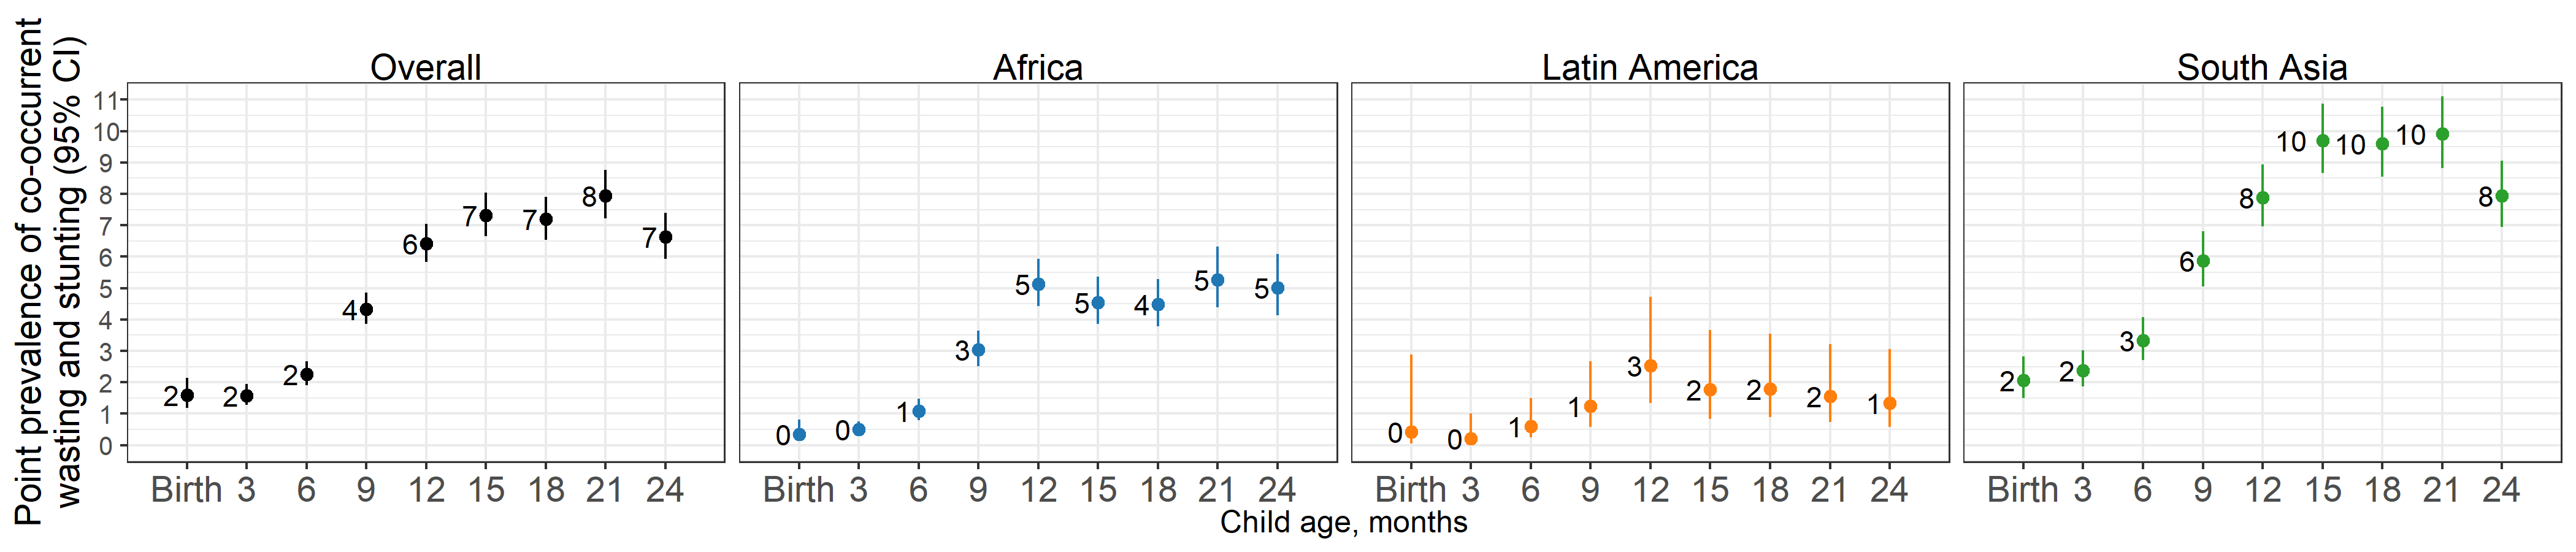
\includegraphics[width=58.33in]{C:/Users/andre/Documents/HBGDki/wasting/ki-longitudinal-manuscripts/figures/wasting/FE/fig-wast-2-co-overall_region--allage-primary_FE}

\hypertarget{cohort}{%
\chapter{Cohort-specific estimates}\label{cohort}}

\raggedright

Below are the cohort-specific estimates for the age-specific prevalences of wasting, severe wasting, persistent wasting, underweight, and concurrent wasting and stunting.

\hypertarget{age-specific-prevalence-1}{%
\section{Age-specific prevalence}\label{age-specific-prevalence-1}}

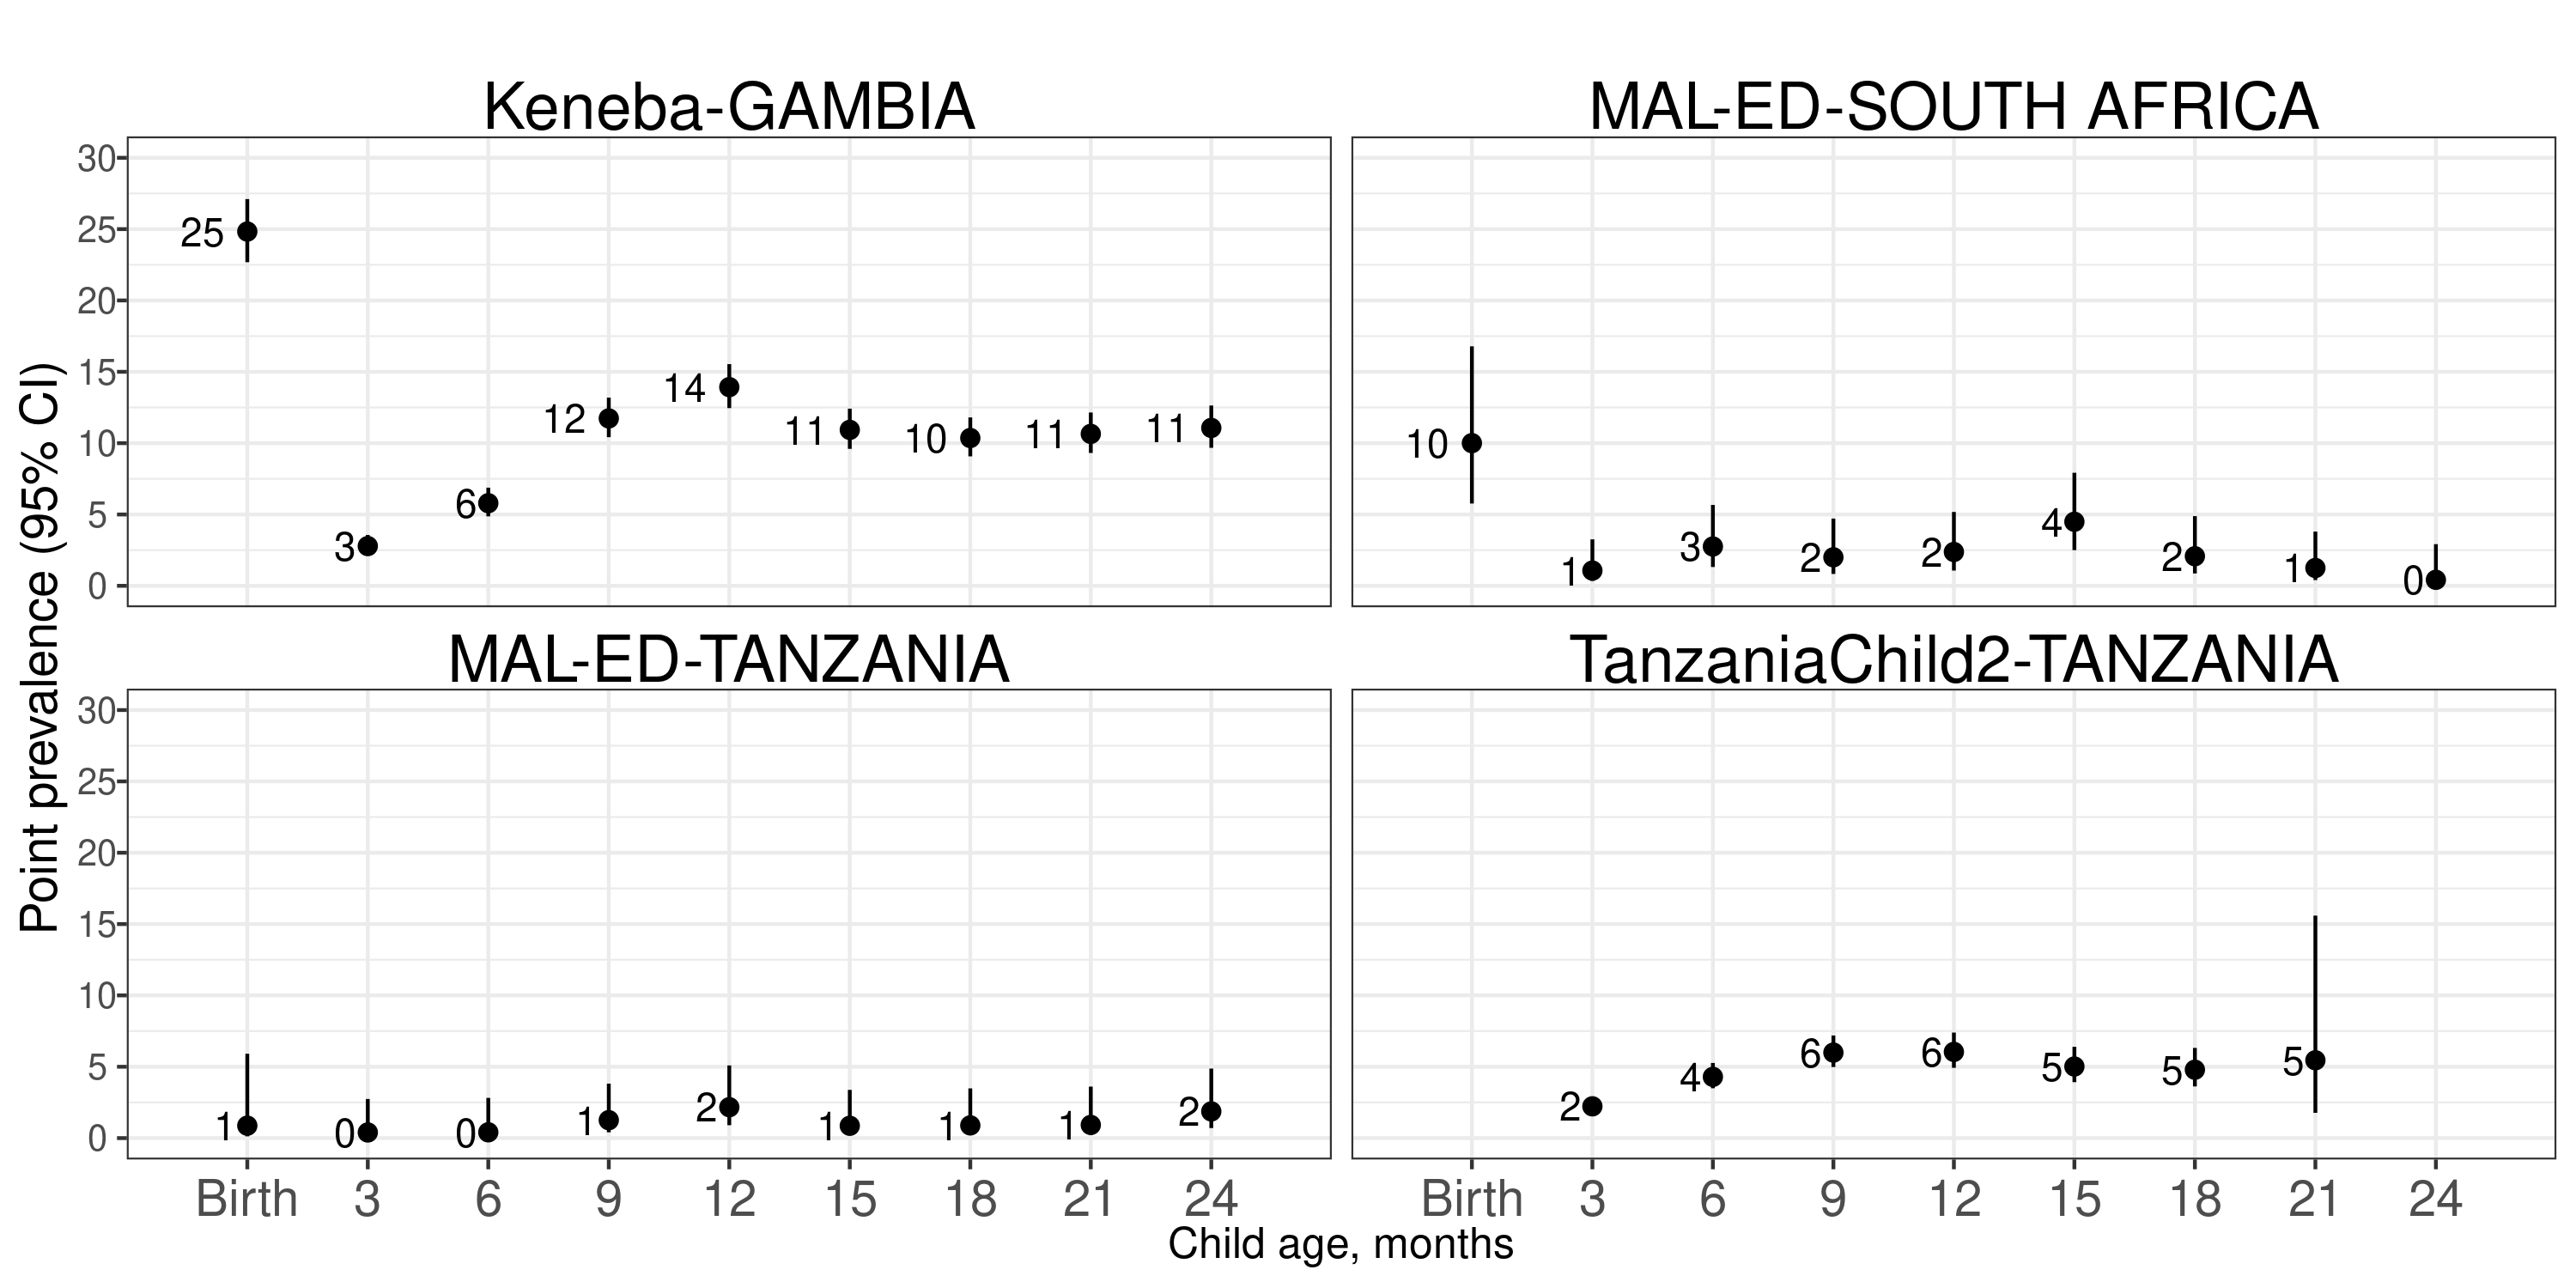
\includegraphics[width=41.67in]{C:/Users/andre/Documents/HBGDki/wasting/ki-longitudinal-manuscripts/figures/wasting/fig-prev_plot_africa}
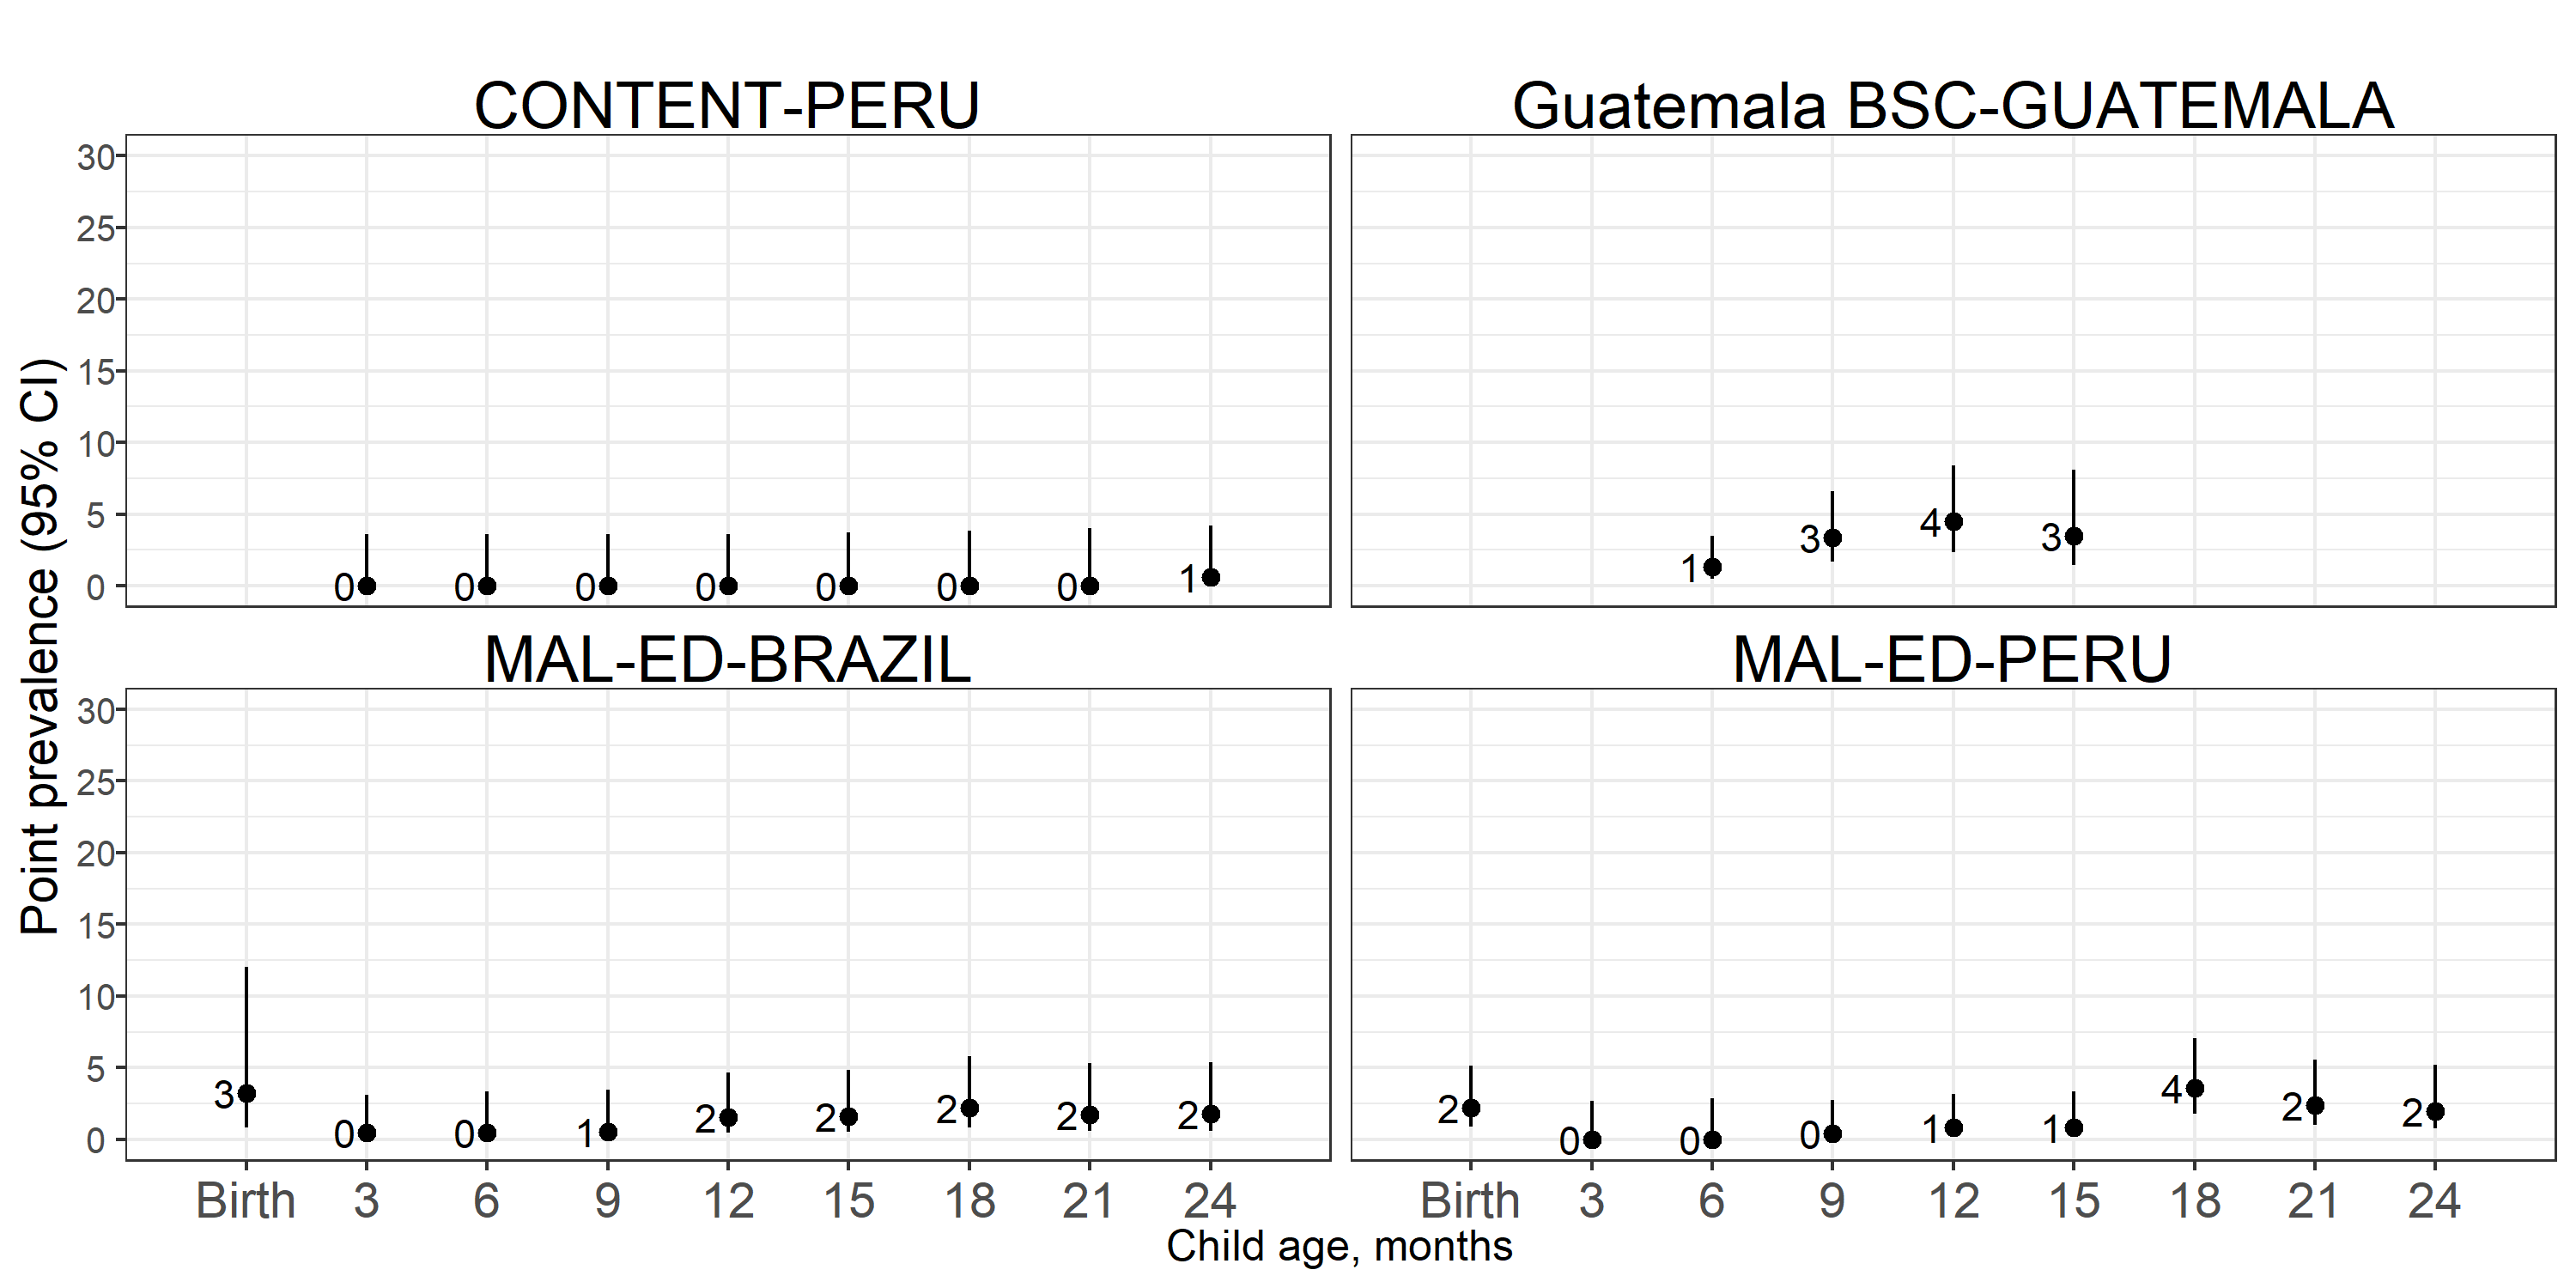
\includegraphics[width=41.67in]{C:/Users/andre/Documents/HBGDki/wasting/ki-longitudinal-manuscripts/figures/wasting/fig-prev_plot_lam}
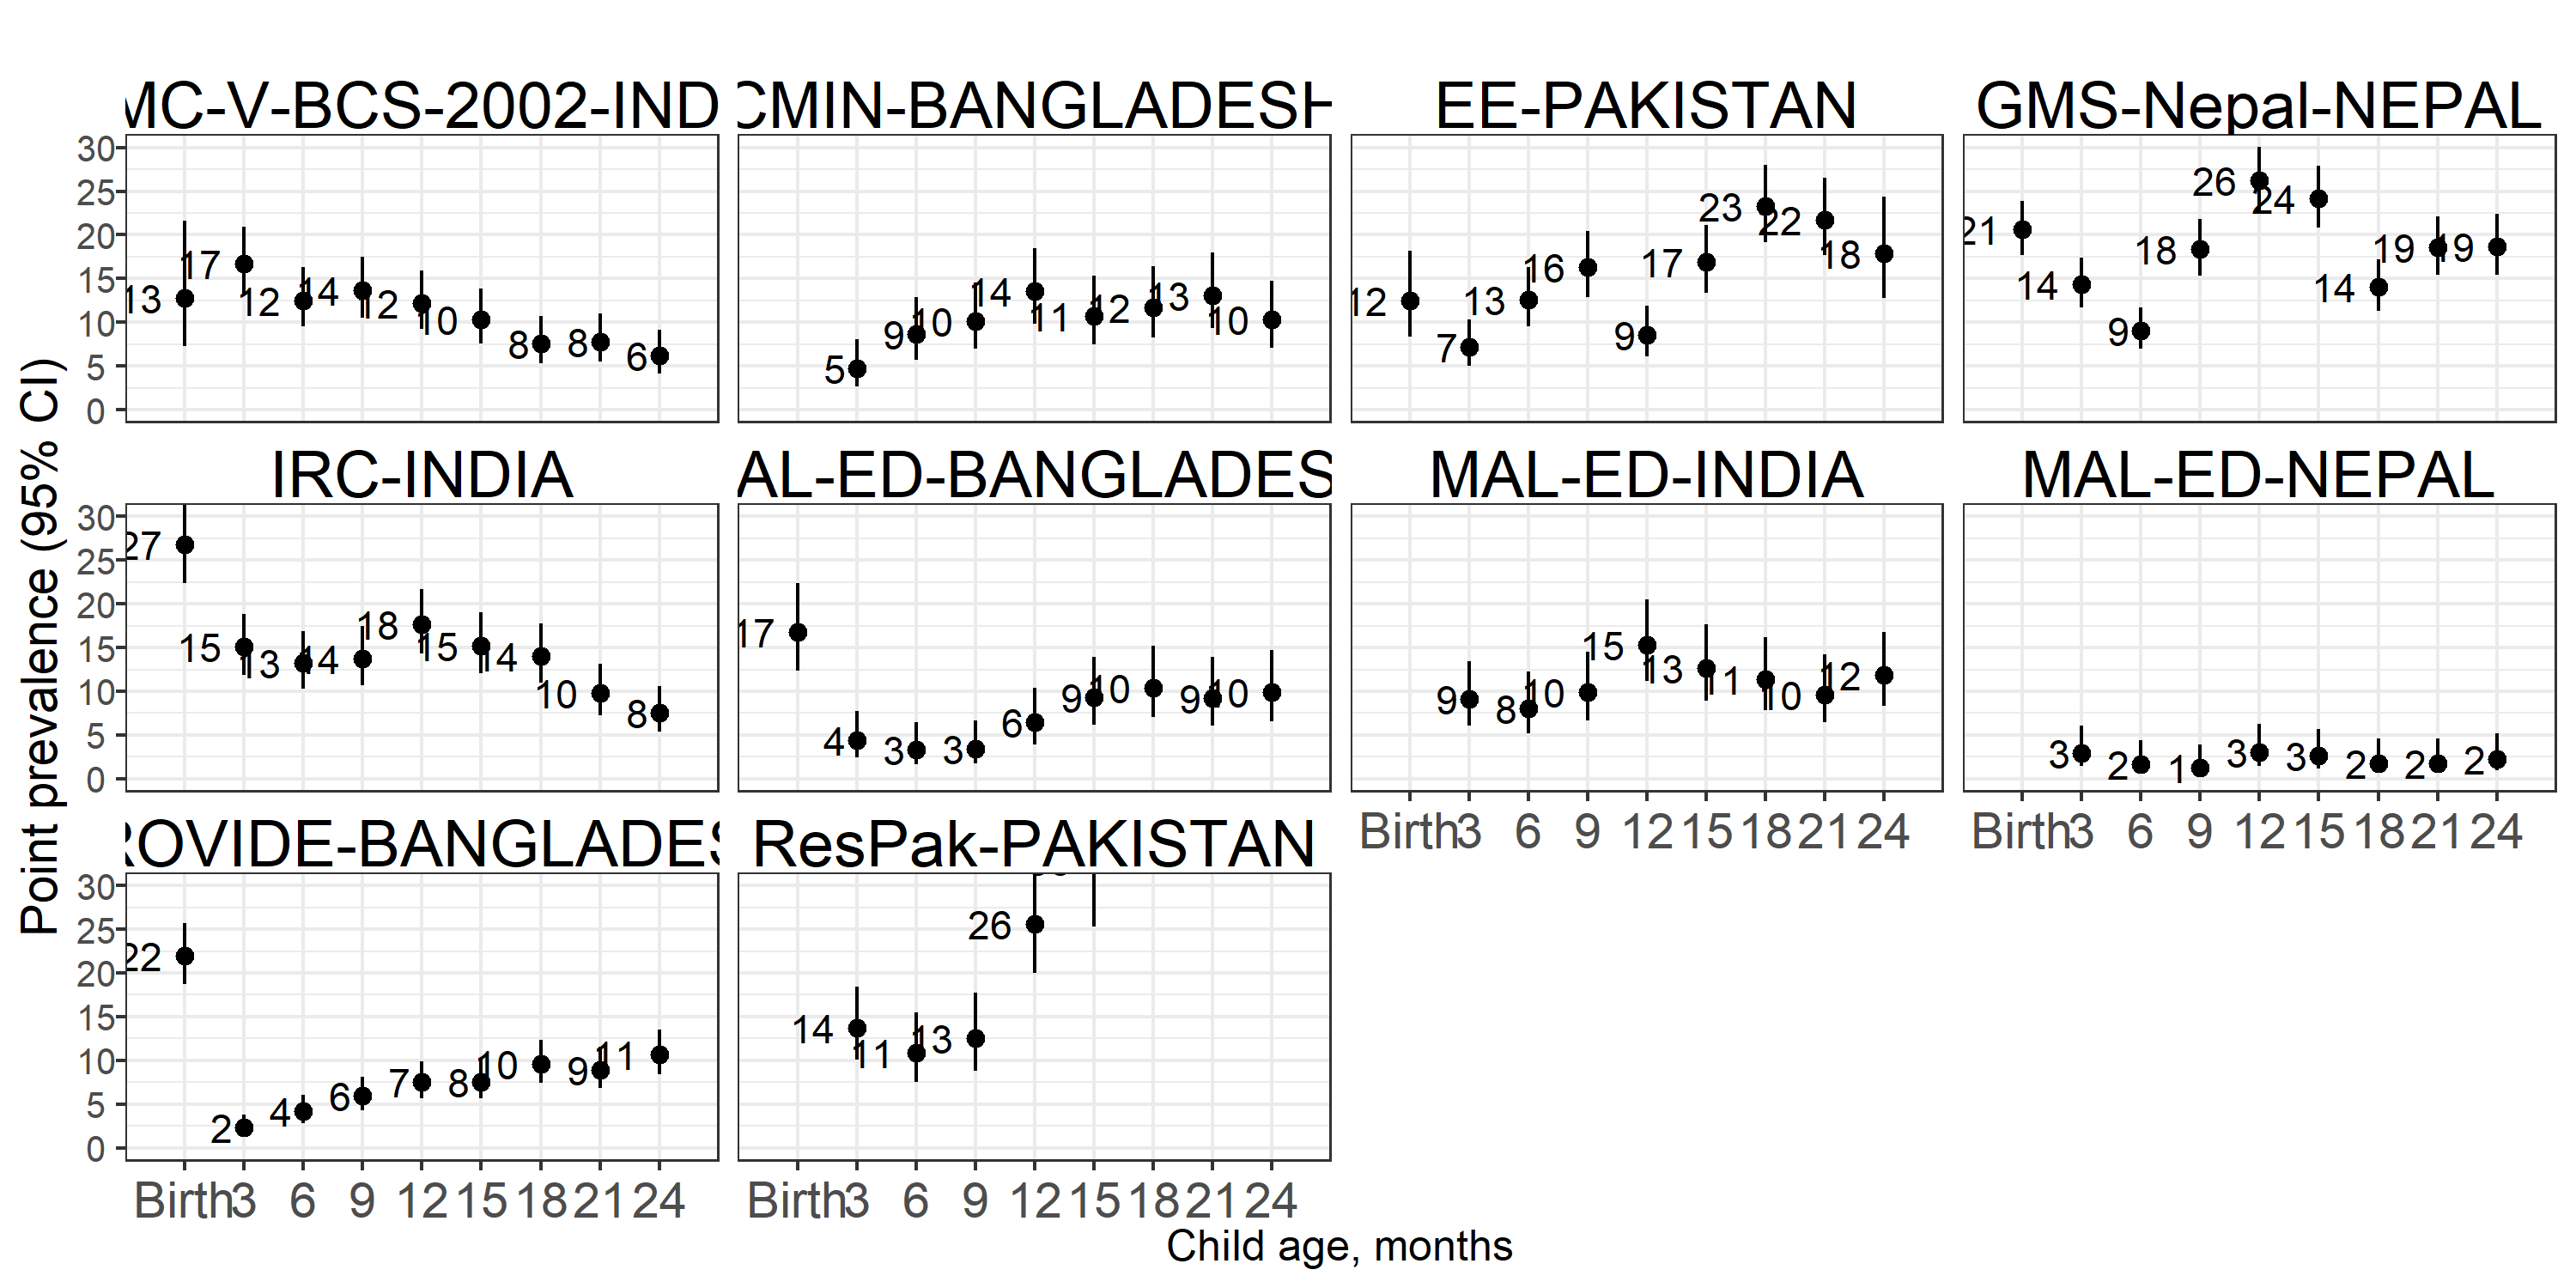
\includegraphics[width=41.67in]{C:/Users/andre/Documents/HBGDki/wasting/ki-longitudinal-manuscripts/figures/wasting/fig-prev_plot_sasia}

\hypertarget{age-specific-prevalence-of-severe-wasting-1}{%
\section{Age-specific prevalence of severe wasting}\label{age-specific-prevalence-of-severe-wasting-1}}

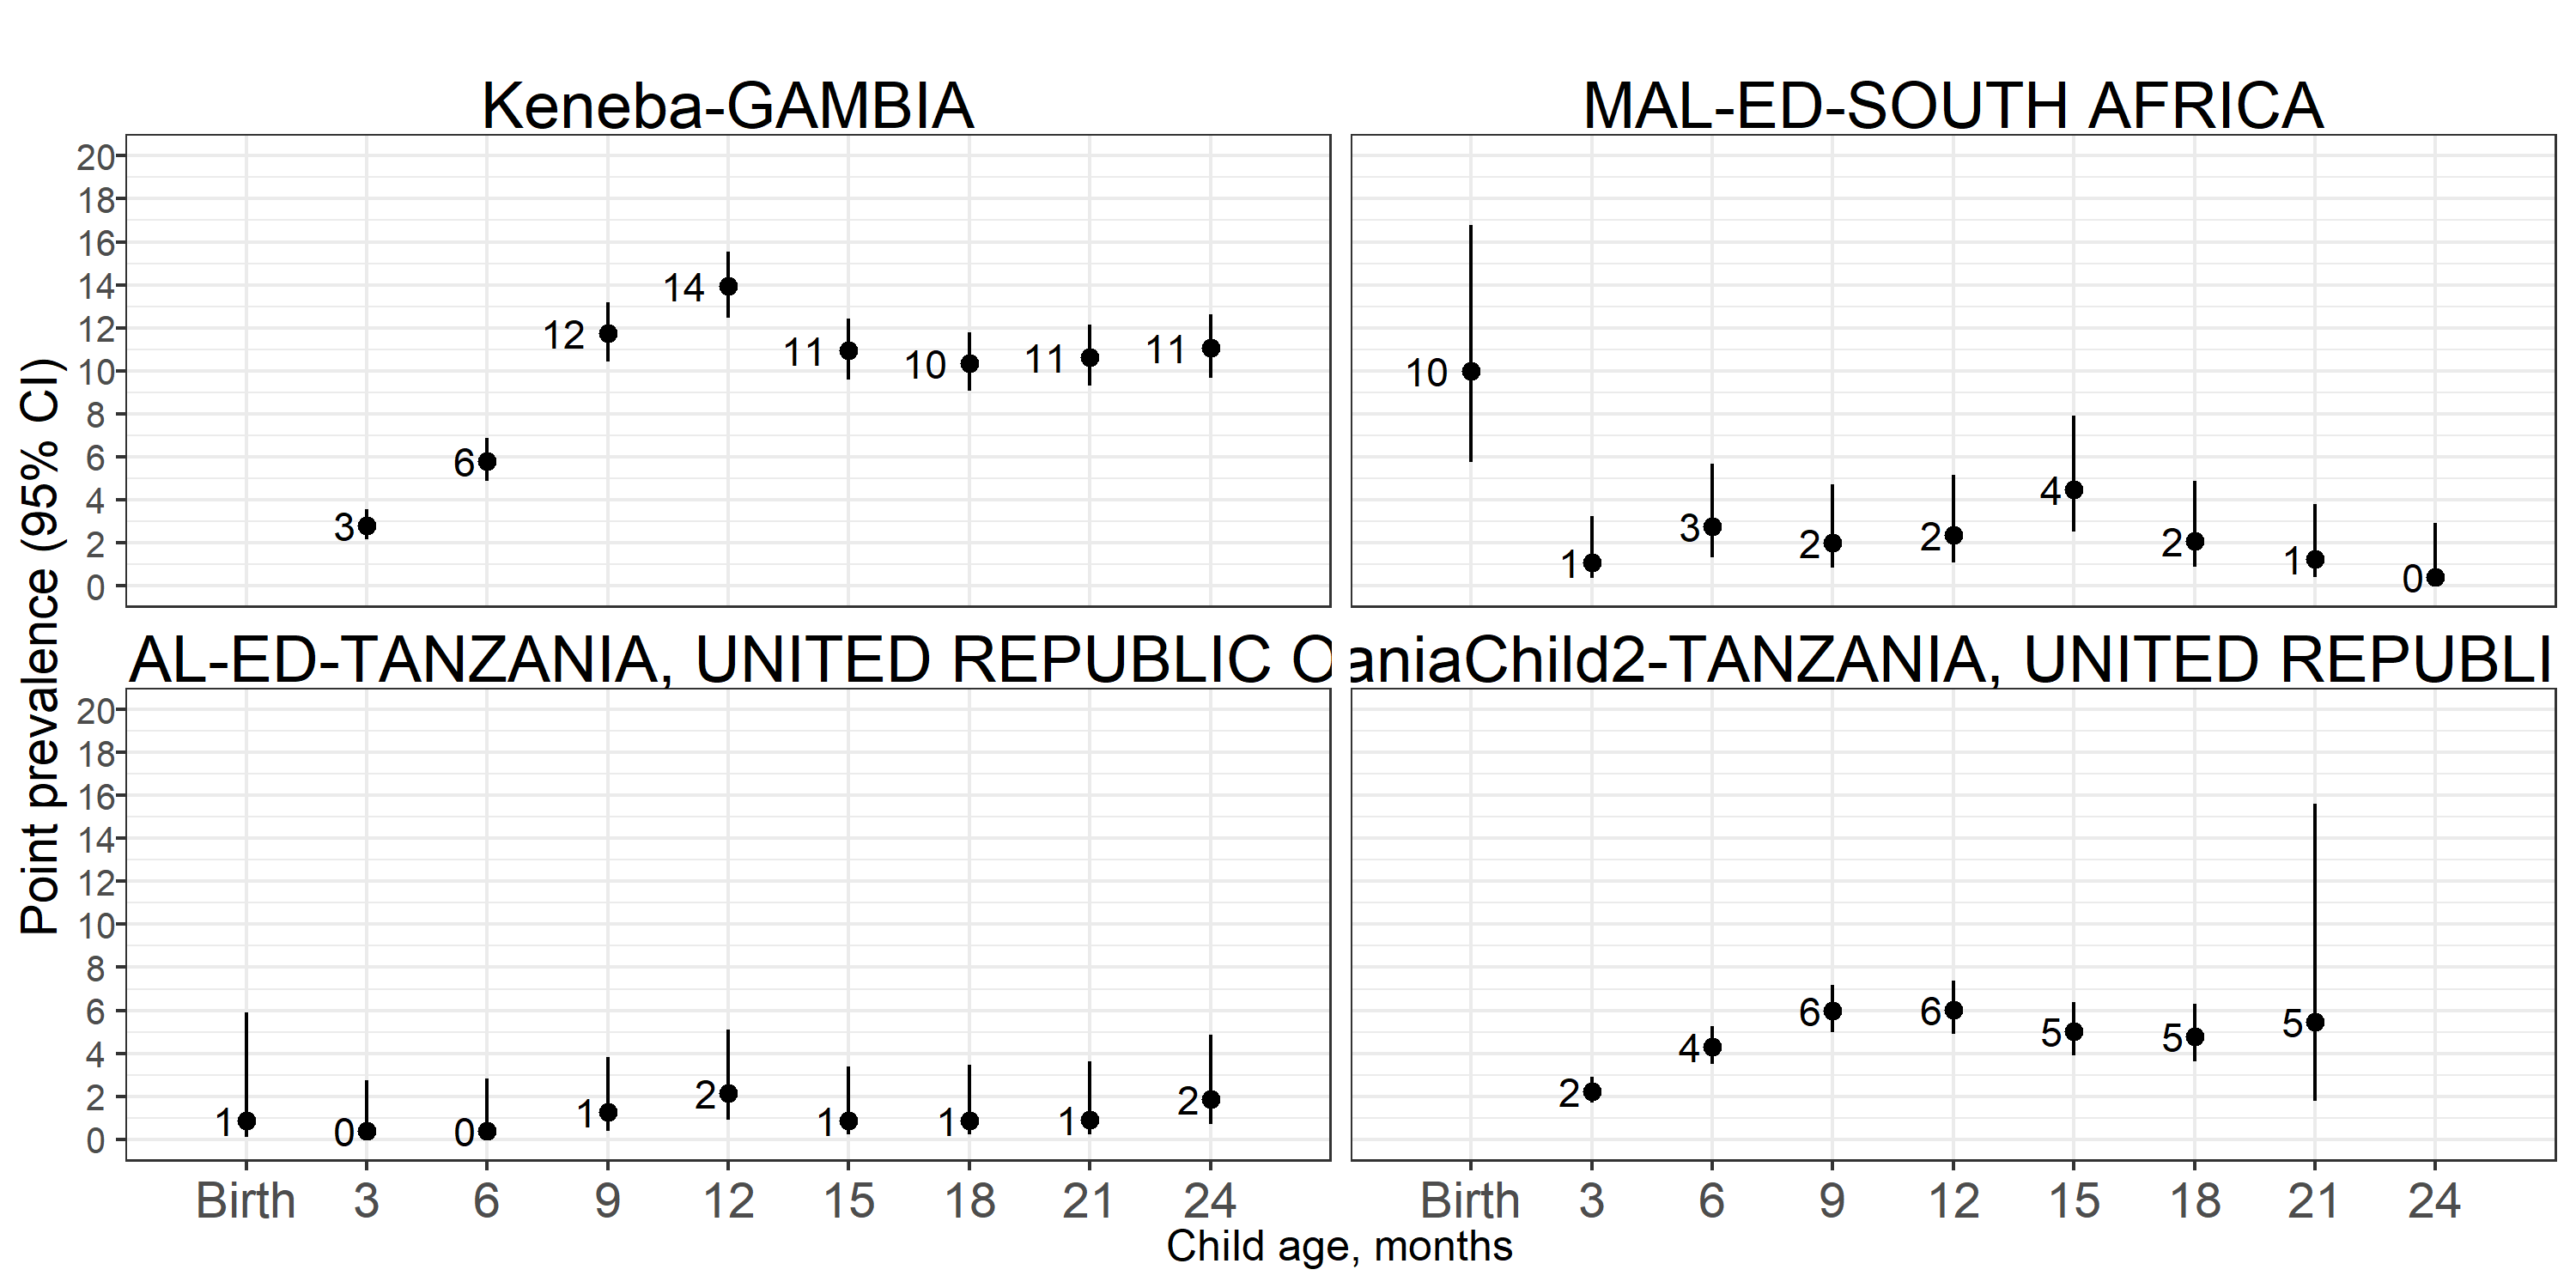
\includegraphics[width=41.67in]{C:/Users/andre/Documents/HBGDki/wasting/ki-longitudinal-manuscripts/figures/wasting/fig-sevwast_plot_africa}
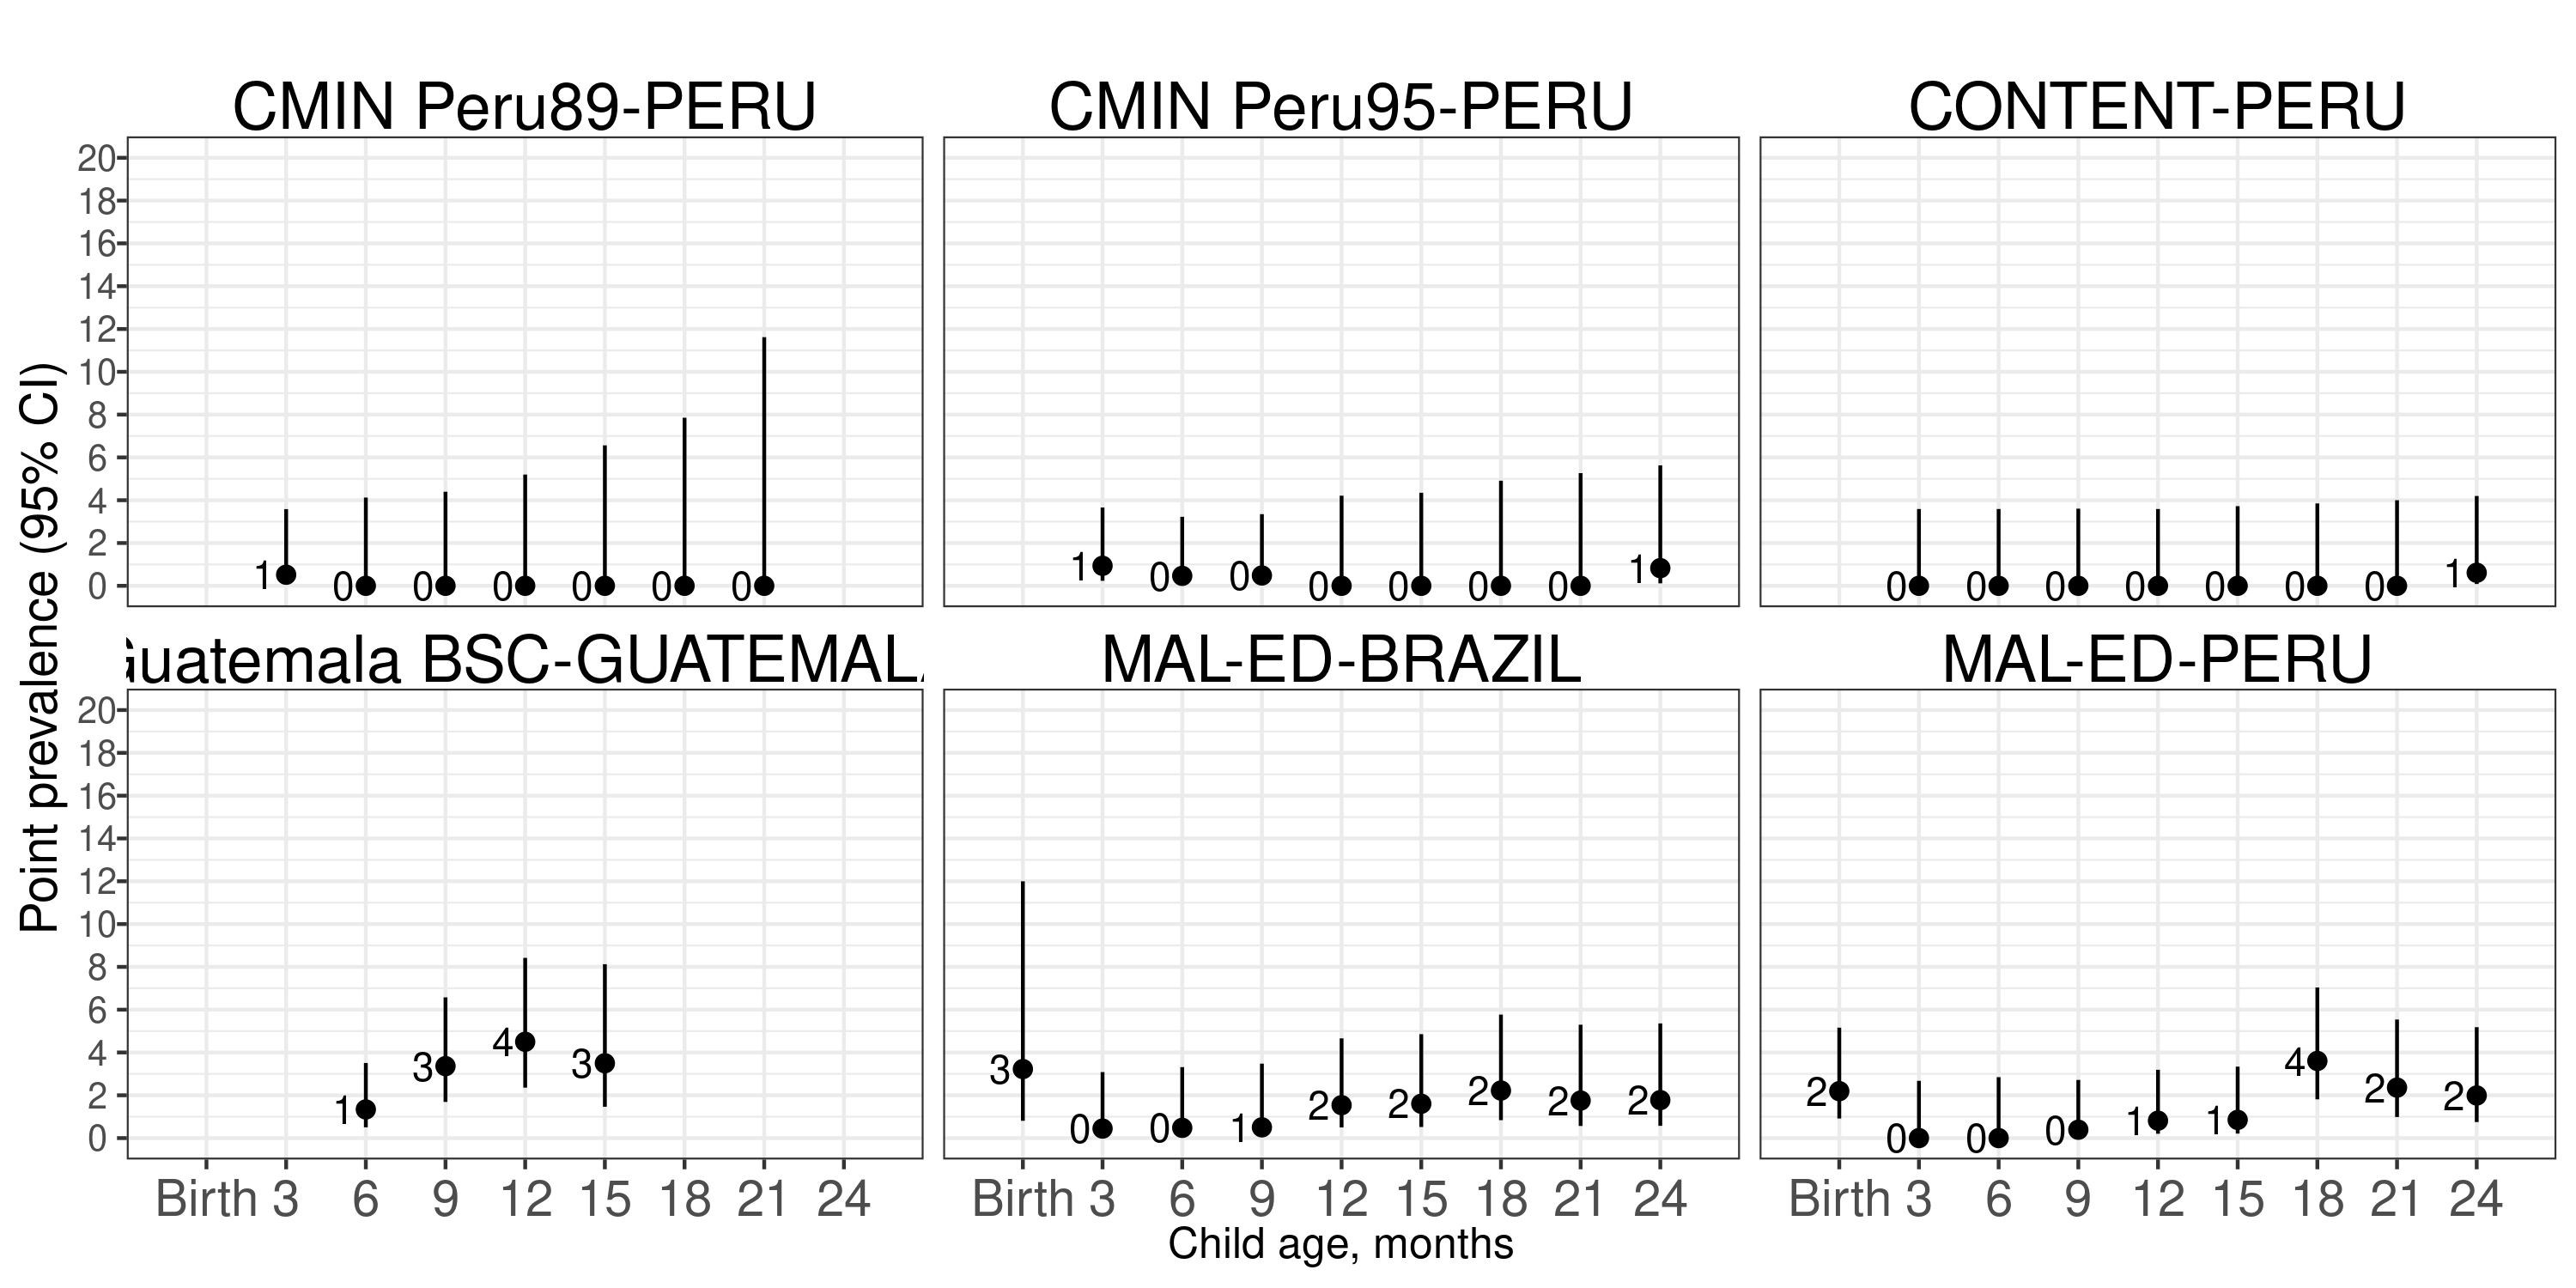
\includegraphics[width=41.67in]{C:/Users/andre/Documents/HBGDki/wasting/ki-longitudinal-manuscripts/figures/wasting/fig-sevwast_plot_lam}
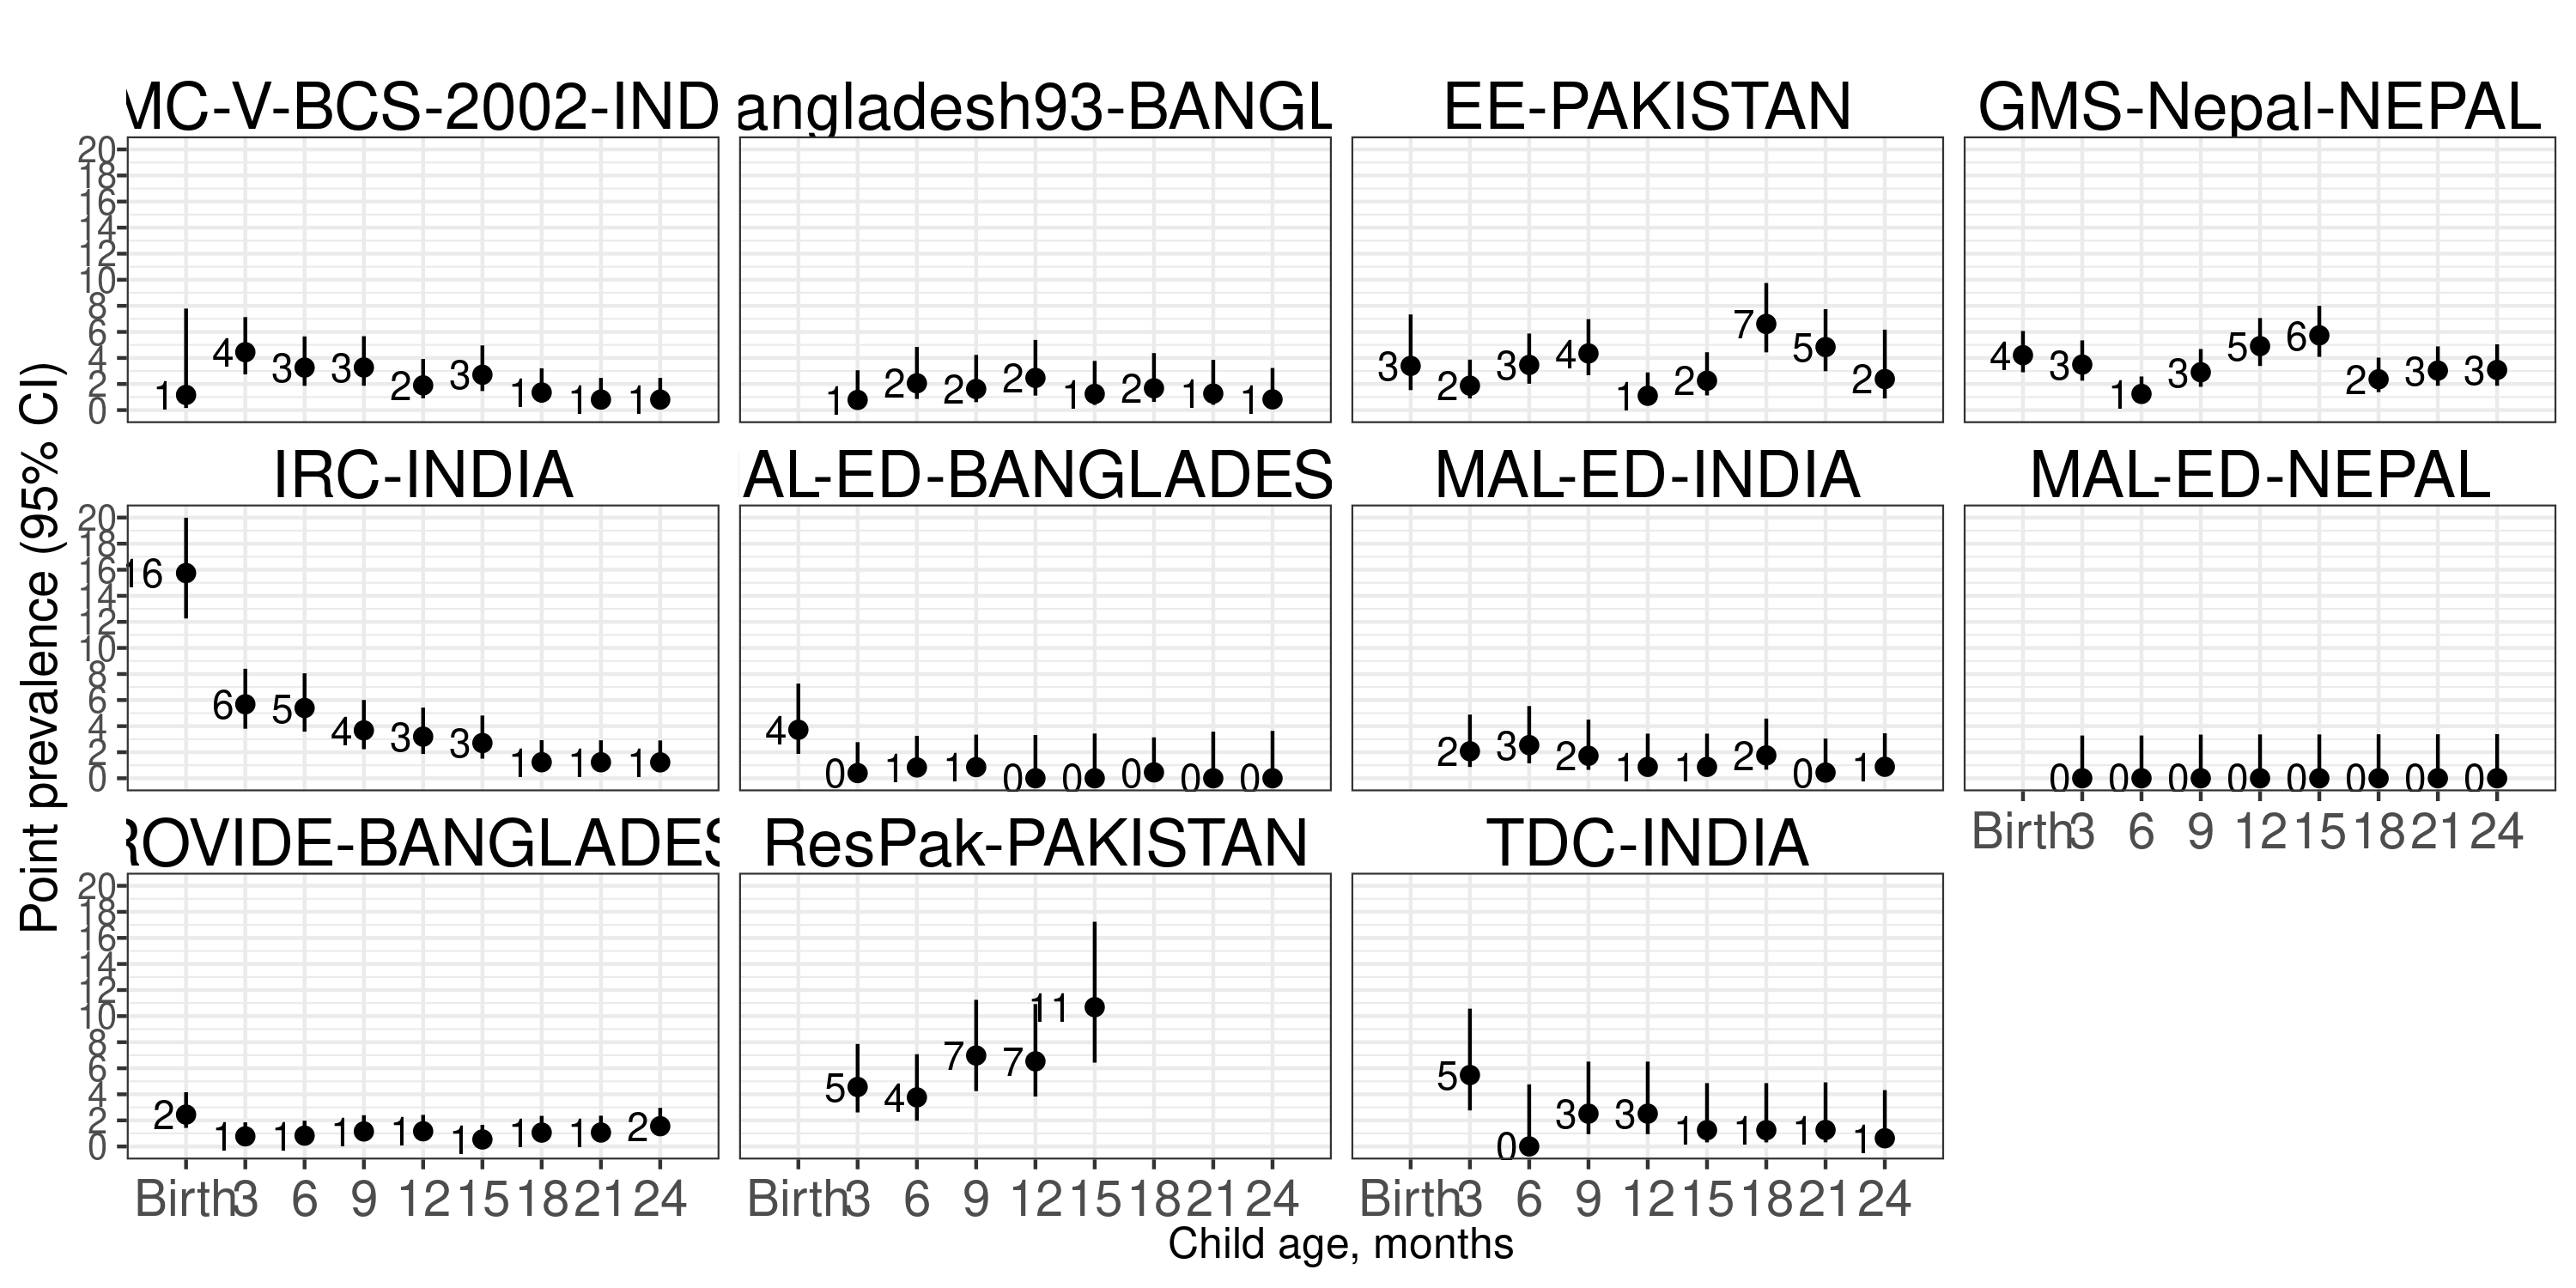
\includegraphics[width=41.67in]{C:/Users/andre/Documents/HBGDki/wasting/ki-longitudinal-manuscripts/figures/wasting/fig-sevwast_plot_sasia}

\hypertarget{age-specific-longitudinal-prevalence-of-persistent-wasting-1}{%
\section{Age-specific longitudinal prevalence of persistent wasting}\label{age-specific-longitudinal-prevalence-of-persistent-wasting-1}}

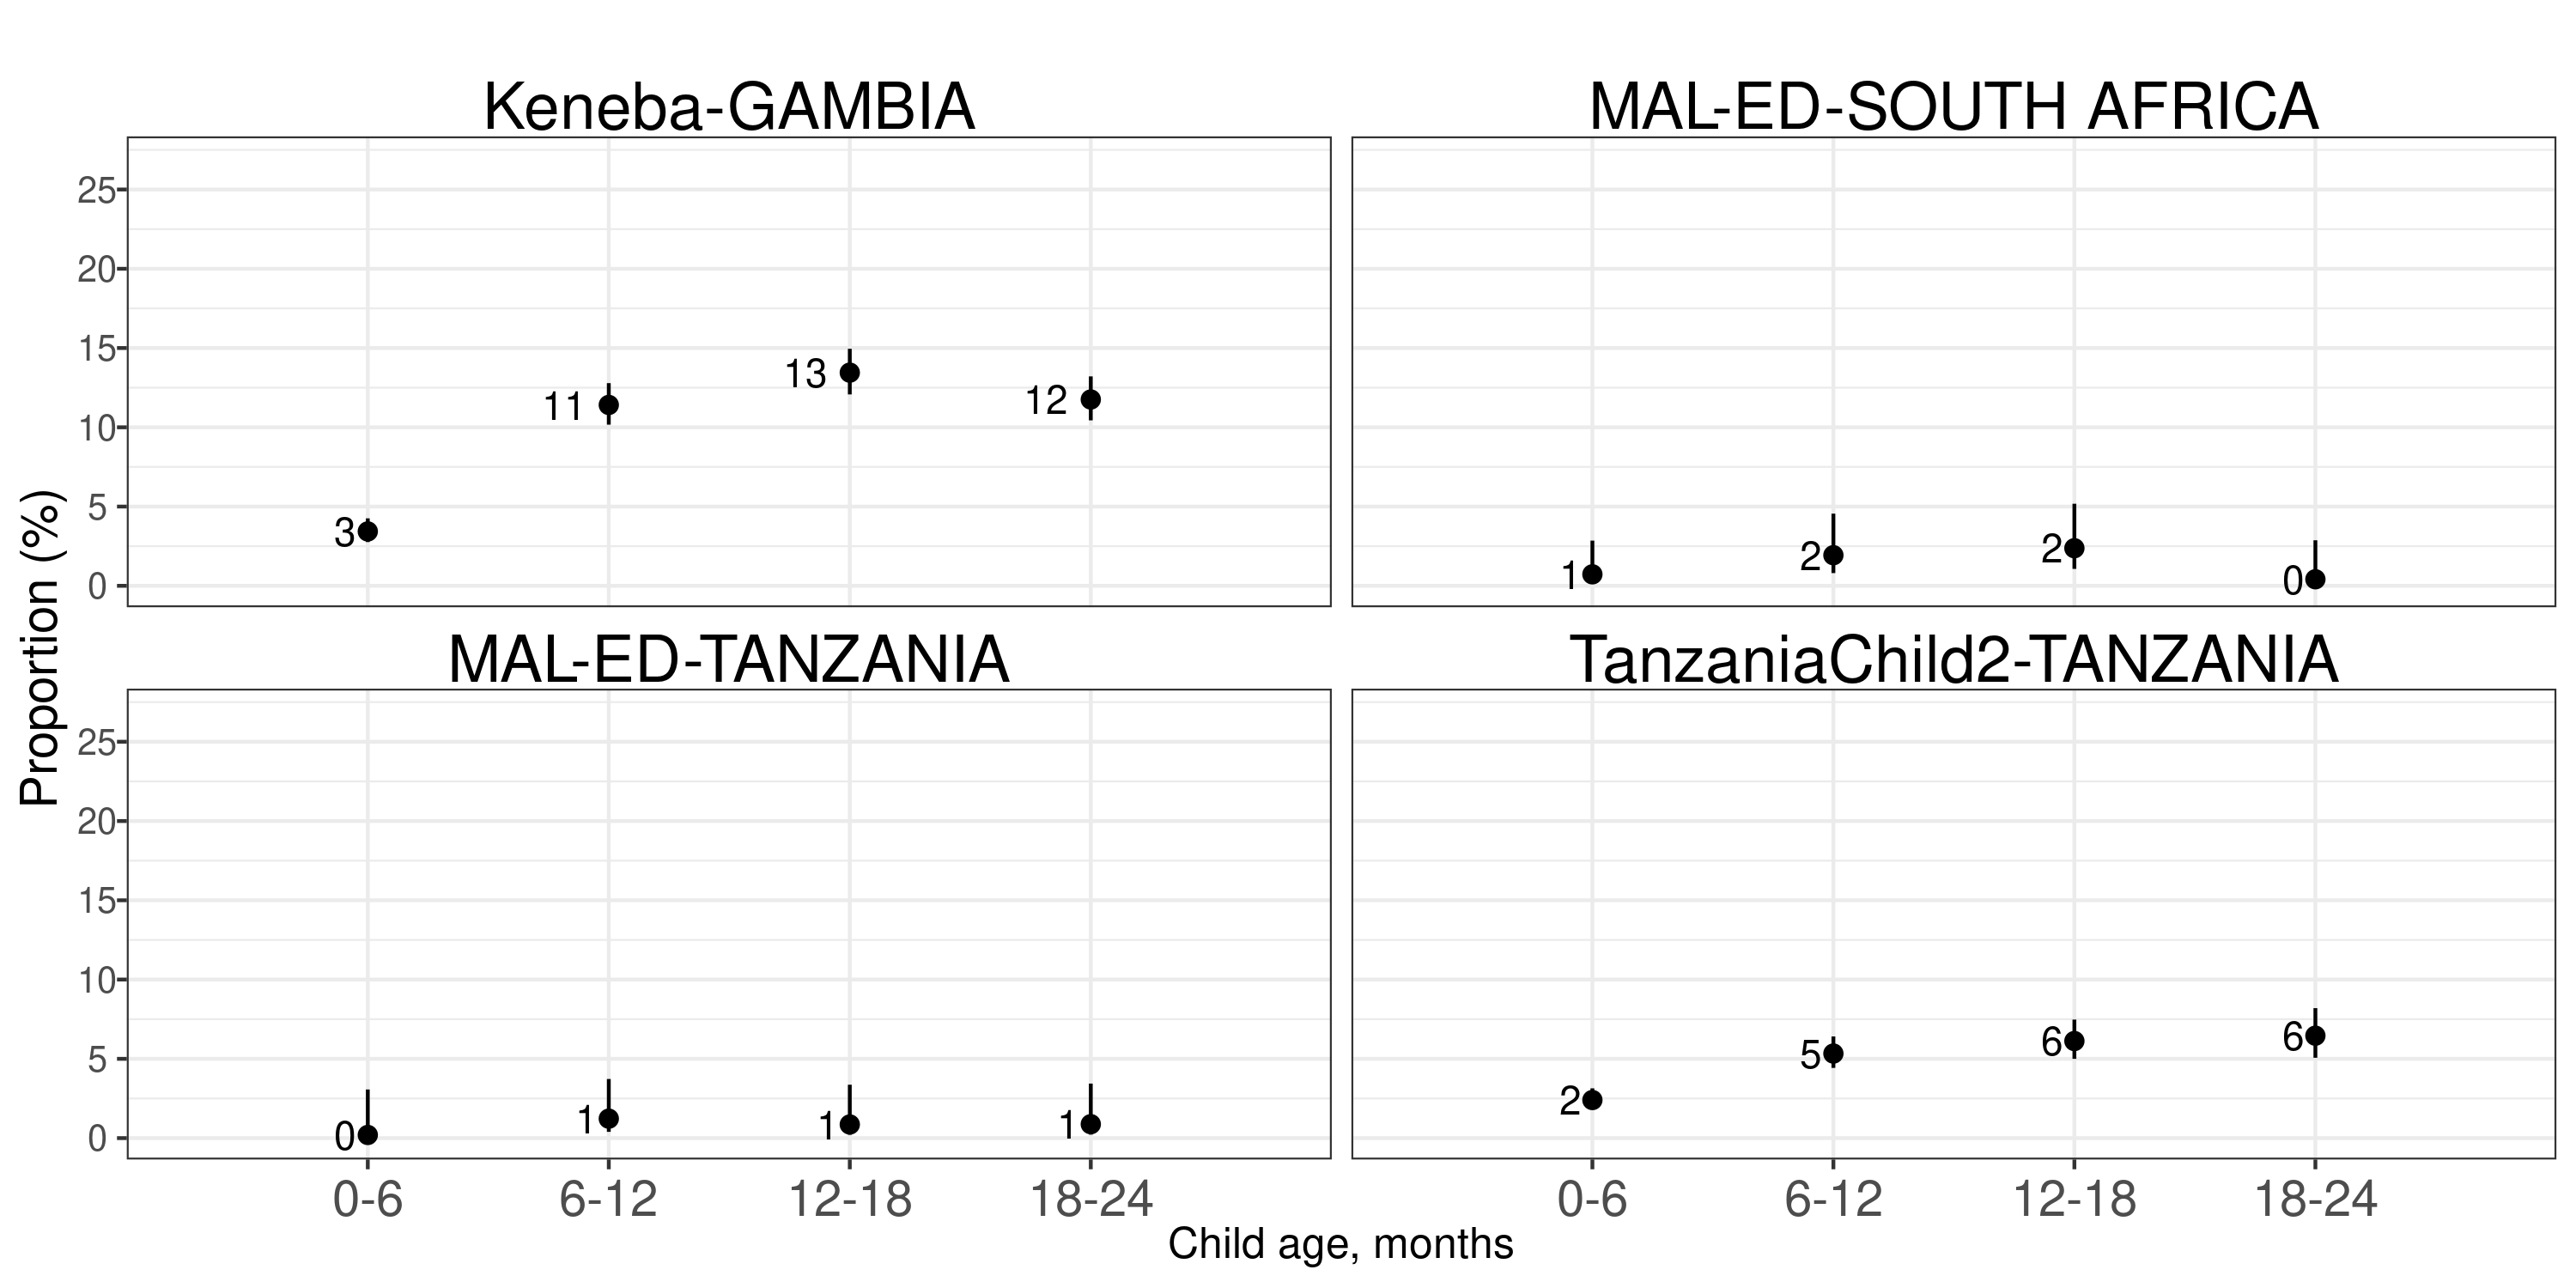
\includegraphics[width=41.67in]{C:/Users/andre/Documents/HBGDki/wasting/ki-longitudinal-manuscripts/figures/wasting/fig-perswast_plot_africa}
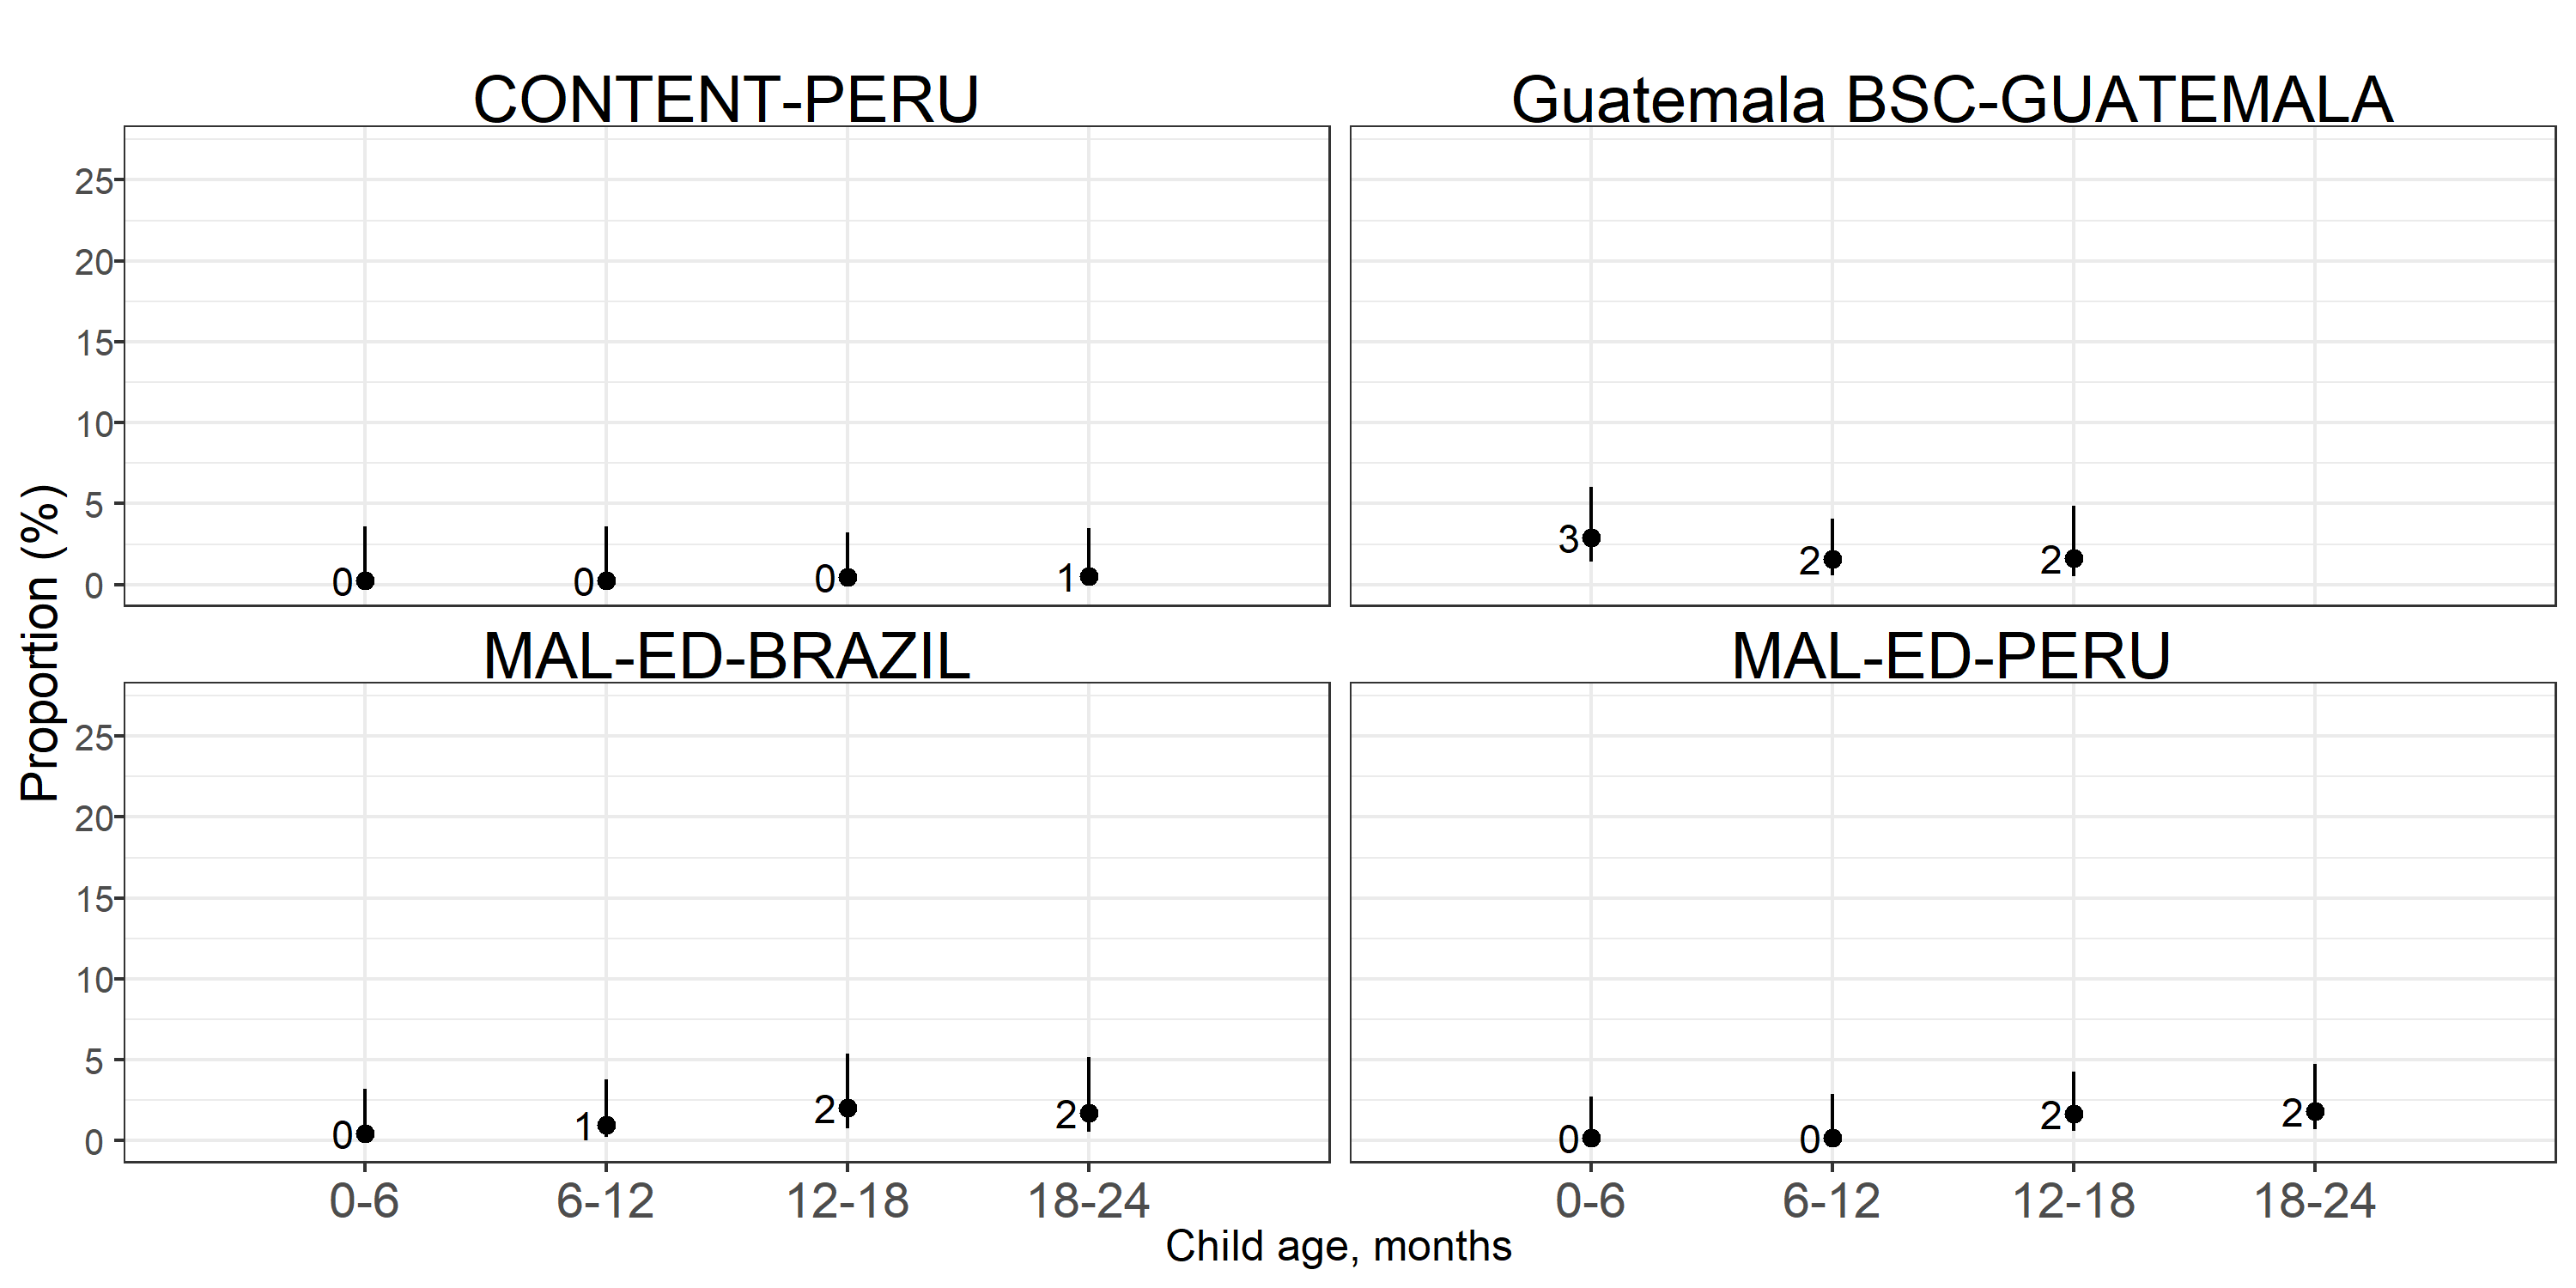
\includegraphics[width=41.67in]{C:/Users/andre/Documents/HBGDki/wasting/ki-longitudinal-manuscripts/figures/wasting/fig-perswast_plot_lam}
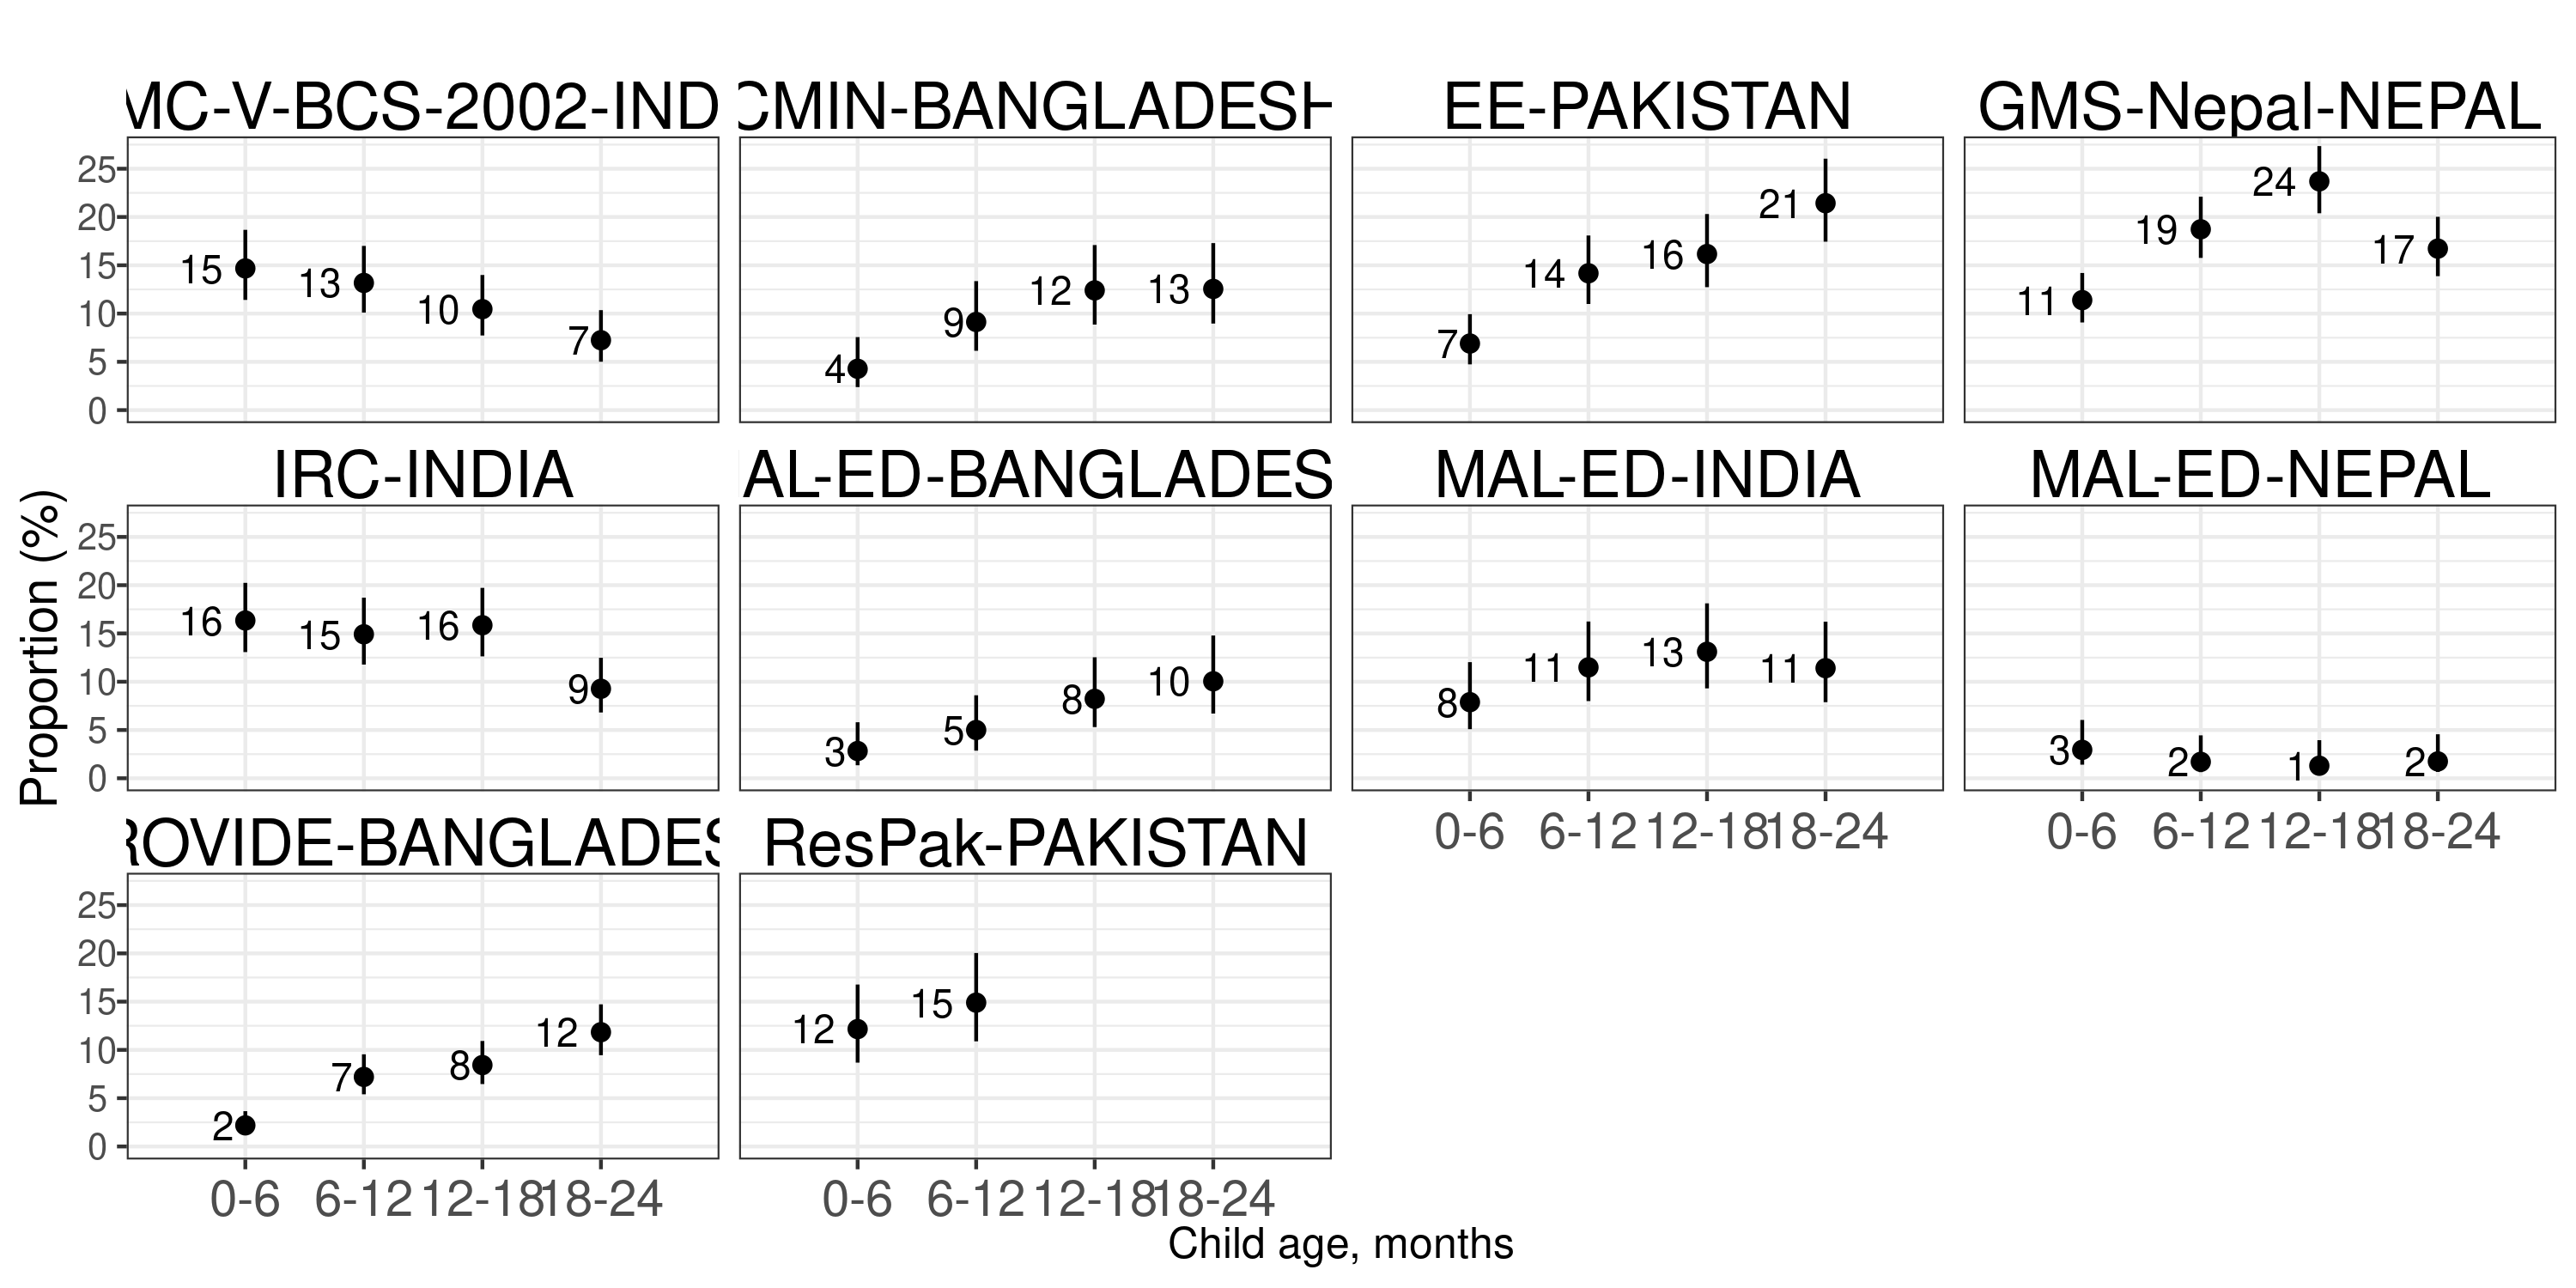
\includegraphics[width=41.67in]{C:/Users/andre/Documents/HBGDki/wasting/ki-longitudinal-manuscripts/figures/wasting/fig-perswast_plot_sasia}

\hypertarget{age-specific-prevalence-of-concurrent-wasting-and-stunting-1}{%
\section{Age-specific prevalence of concurrent wasting and stunting}\label{age-specific-prevalence-of-concurrent-wasting-and-stunting-1}}

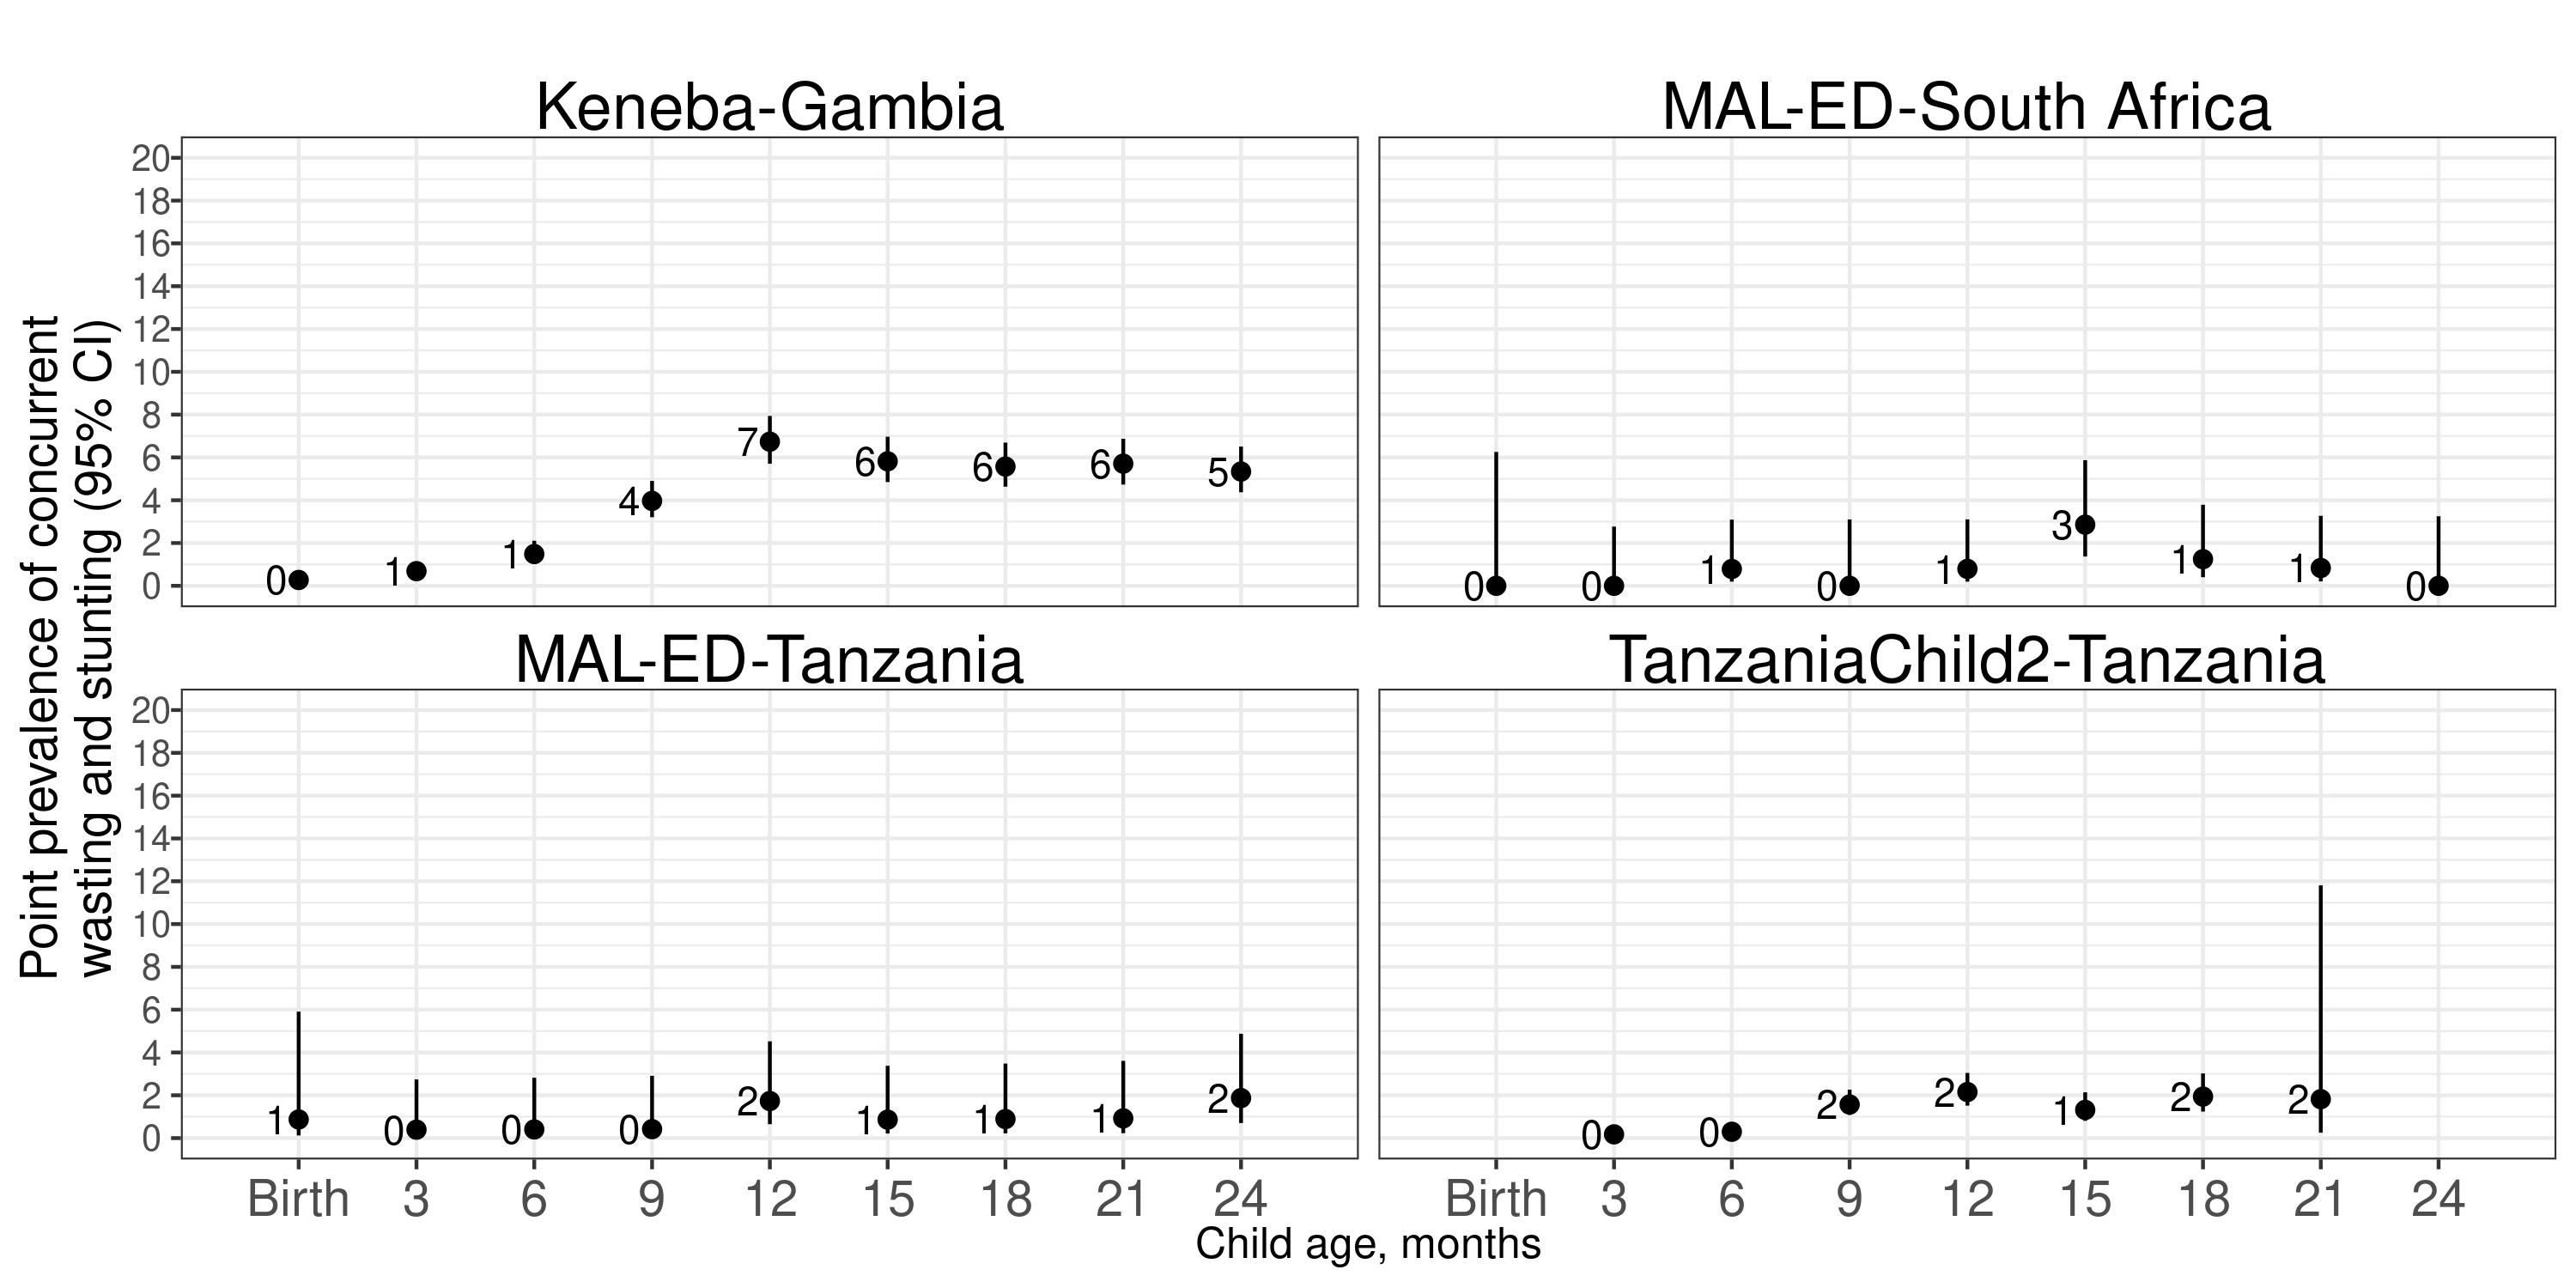
\includegraphics[width=41.67in]{C:/Users/andre/Documents/HBGDki/wasting/ki-longitudinal-manuscripts/figures/wasting/fig-co_plot_africa}
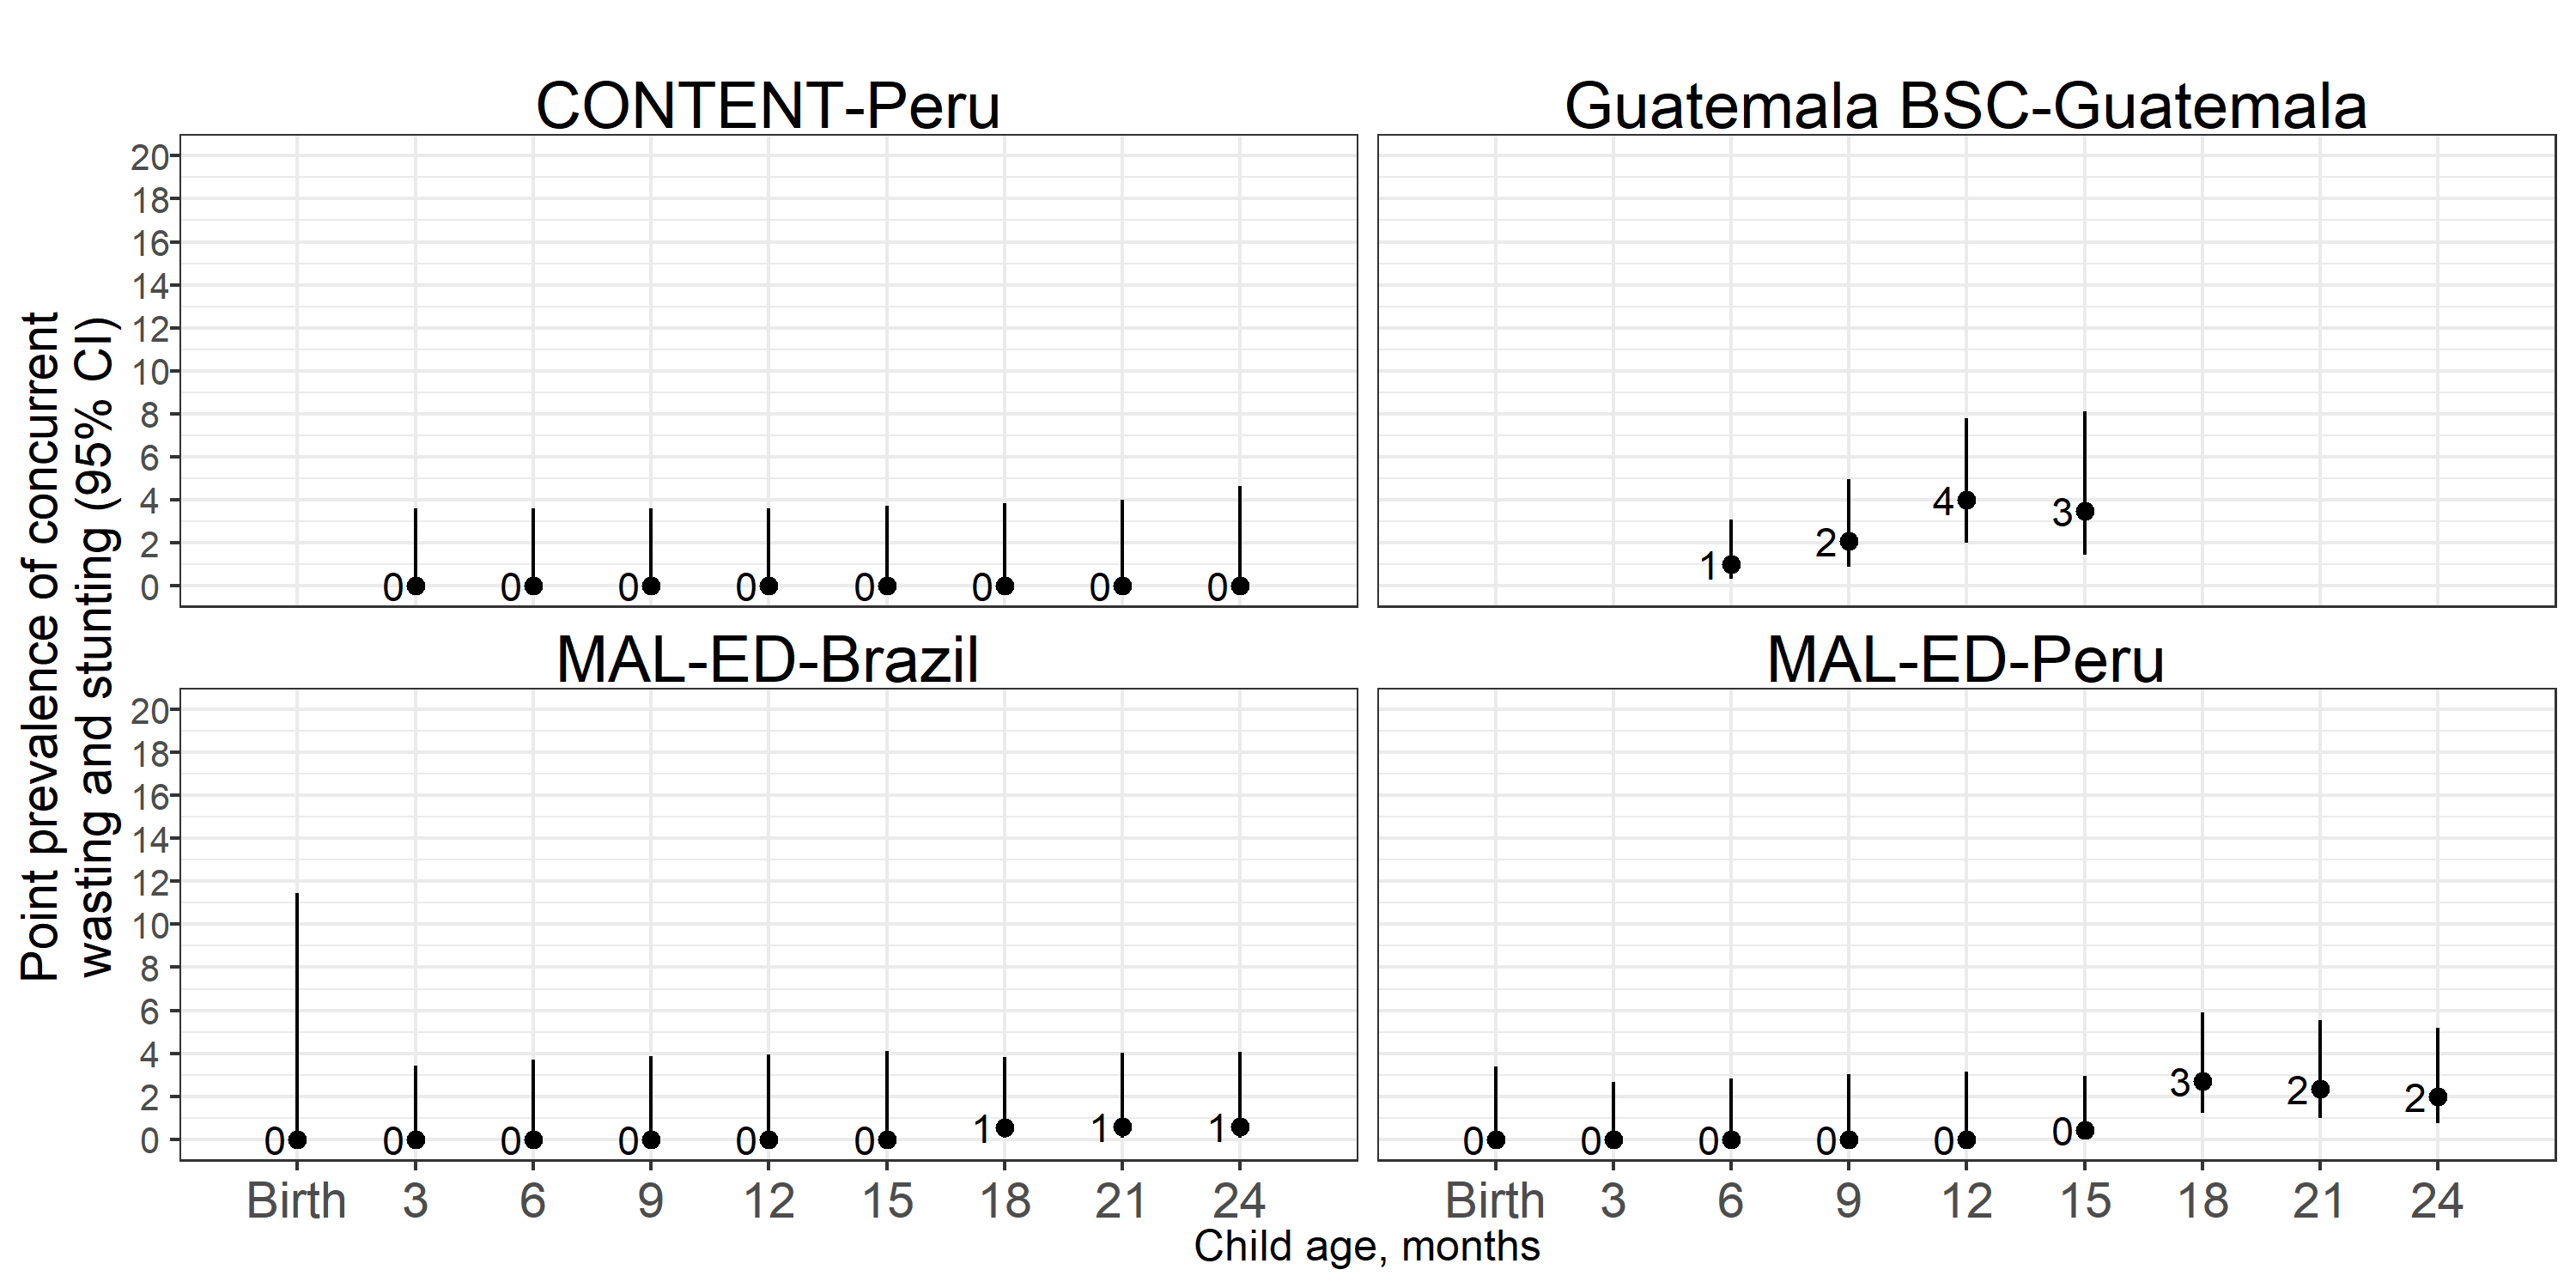
\includegraphics[width=41.67in]{C:/Users/andre/Documents/HBGDki/wasting/ki-longitudinal-manuscripts/figures/wasting/fig-co_plot_lam}
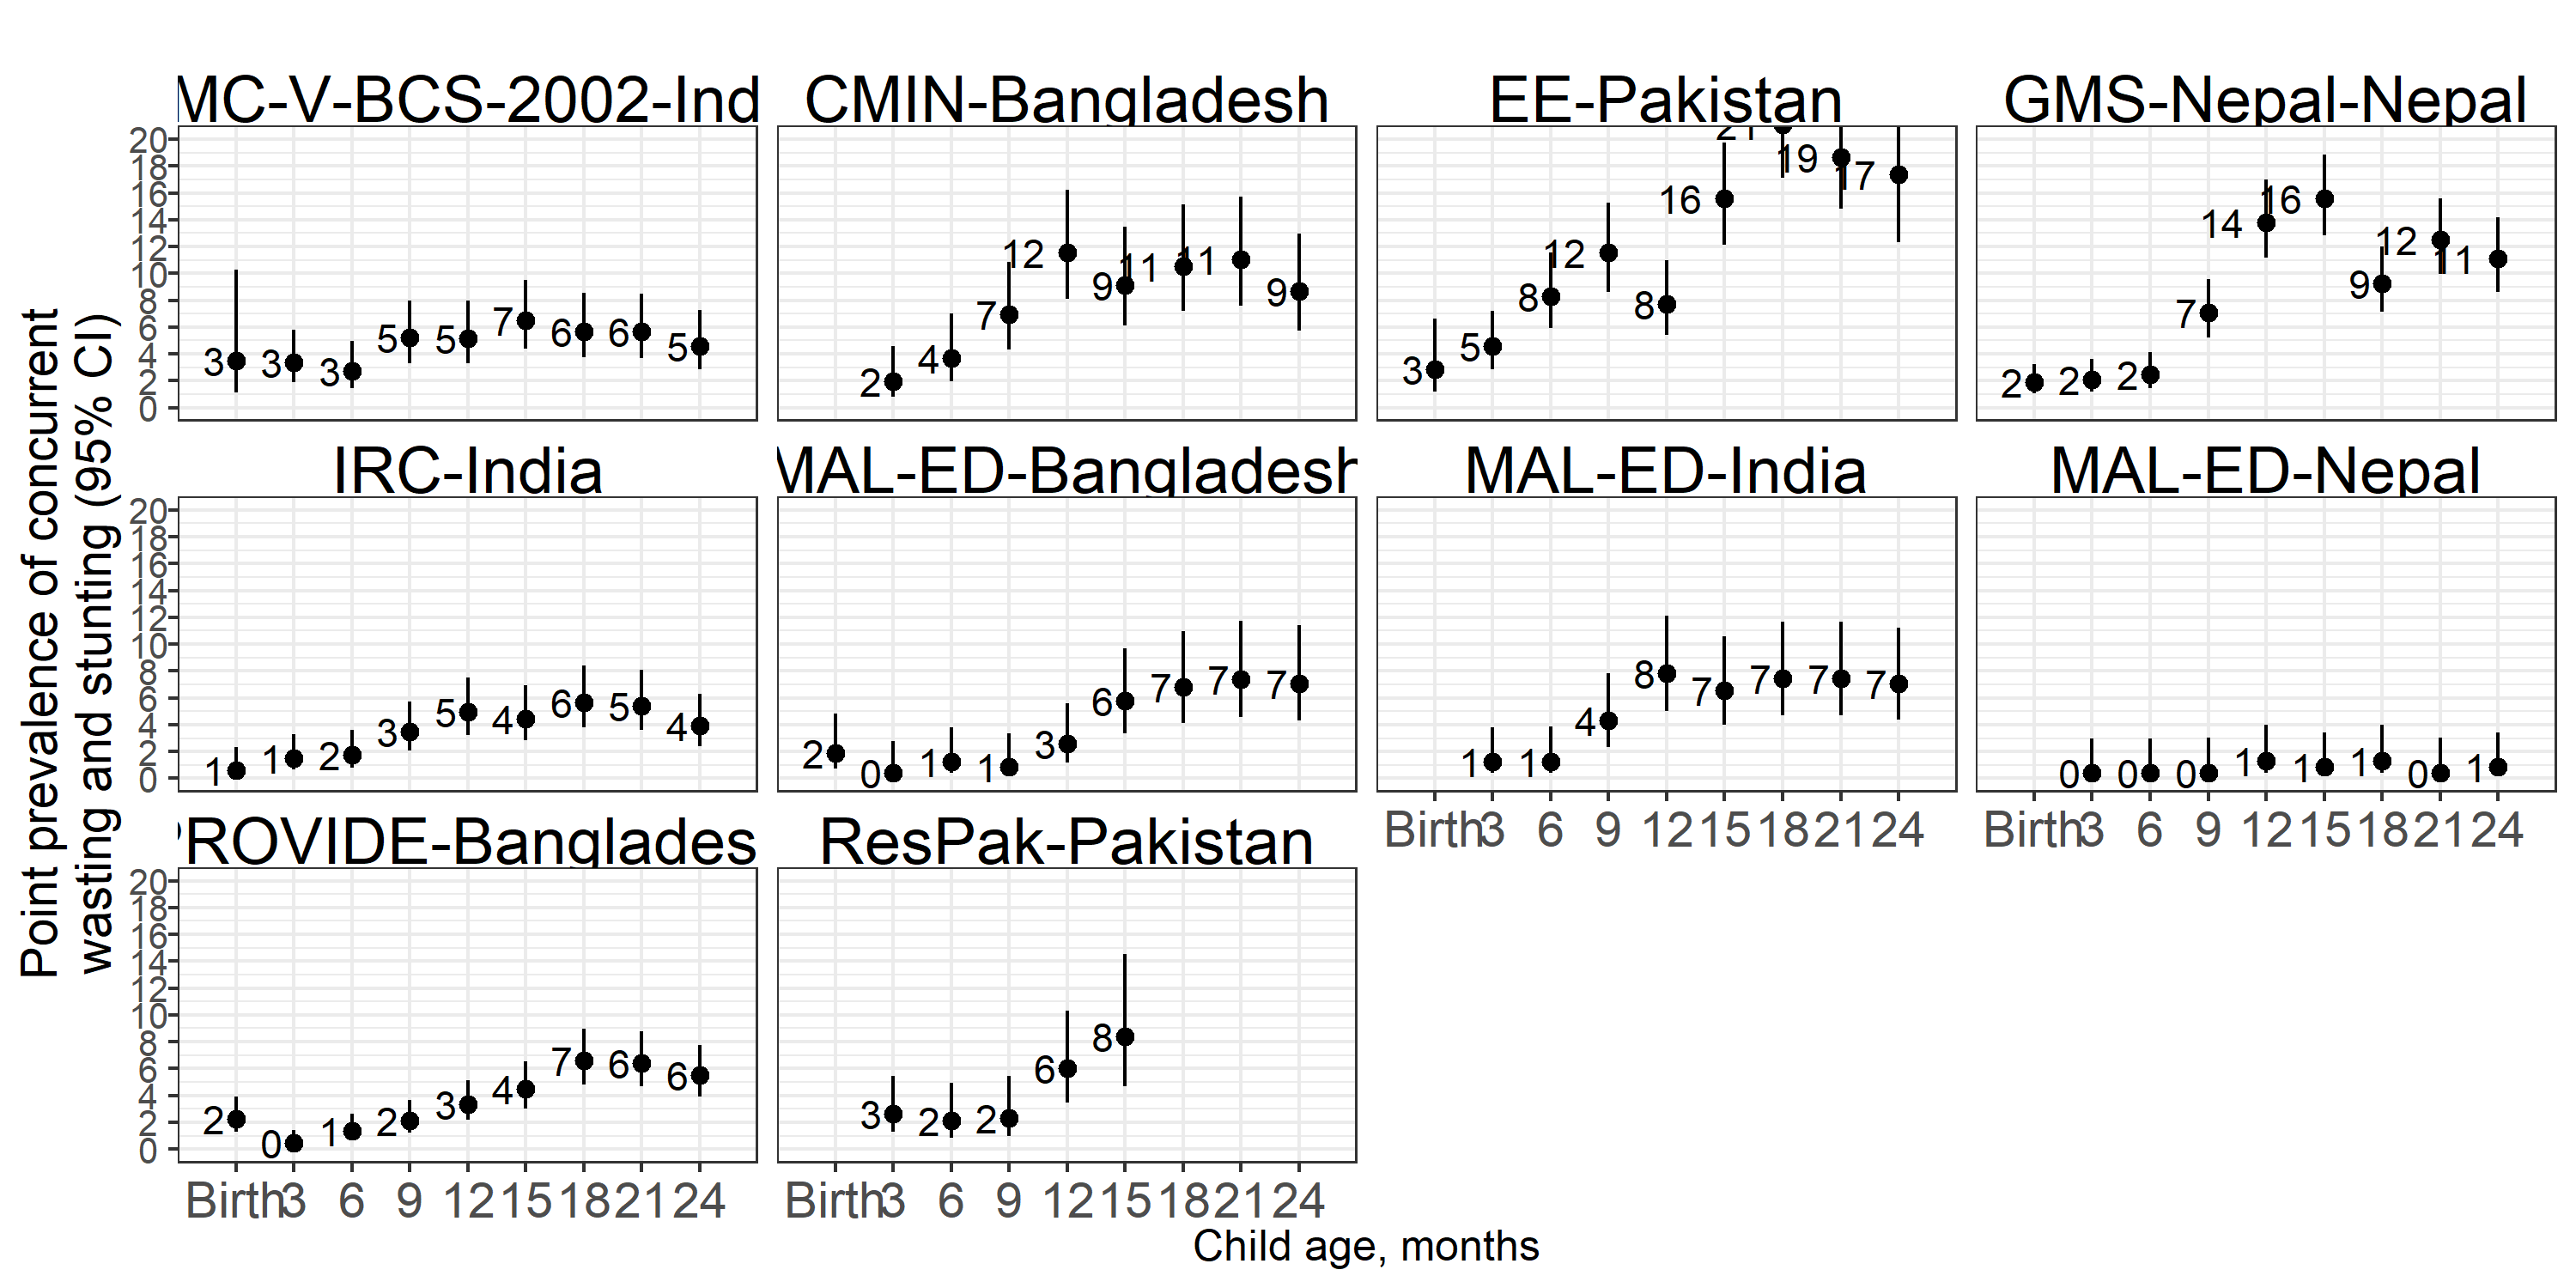
\includegraphics[width=41.67in]{C:/Users/andre/Documents/HBGDki/wasting/ki-longitudinal-manuscripts/figures/wasting/fig-co_plot_sasia}

\hypertarget{age-specific-prevalence-of-underweight-weight-for-age-z-score--2}{%
\section{Age-specific prevalence of underweight (weight-for-age Z-score \textless{} -2)}\label{age-specific-prevalence-of-underweight-weight-for-age-z-score--2}}

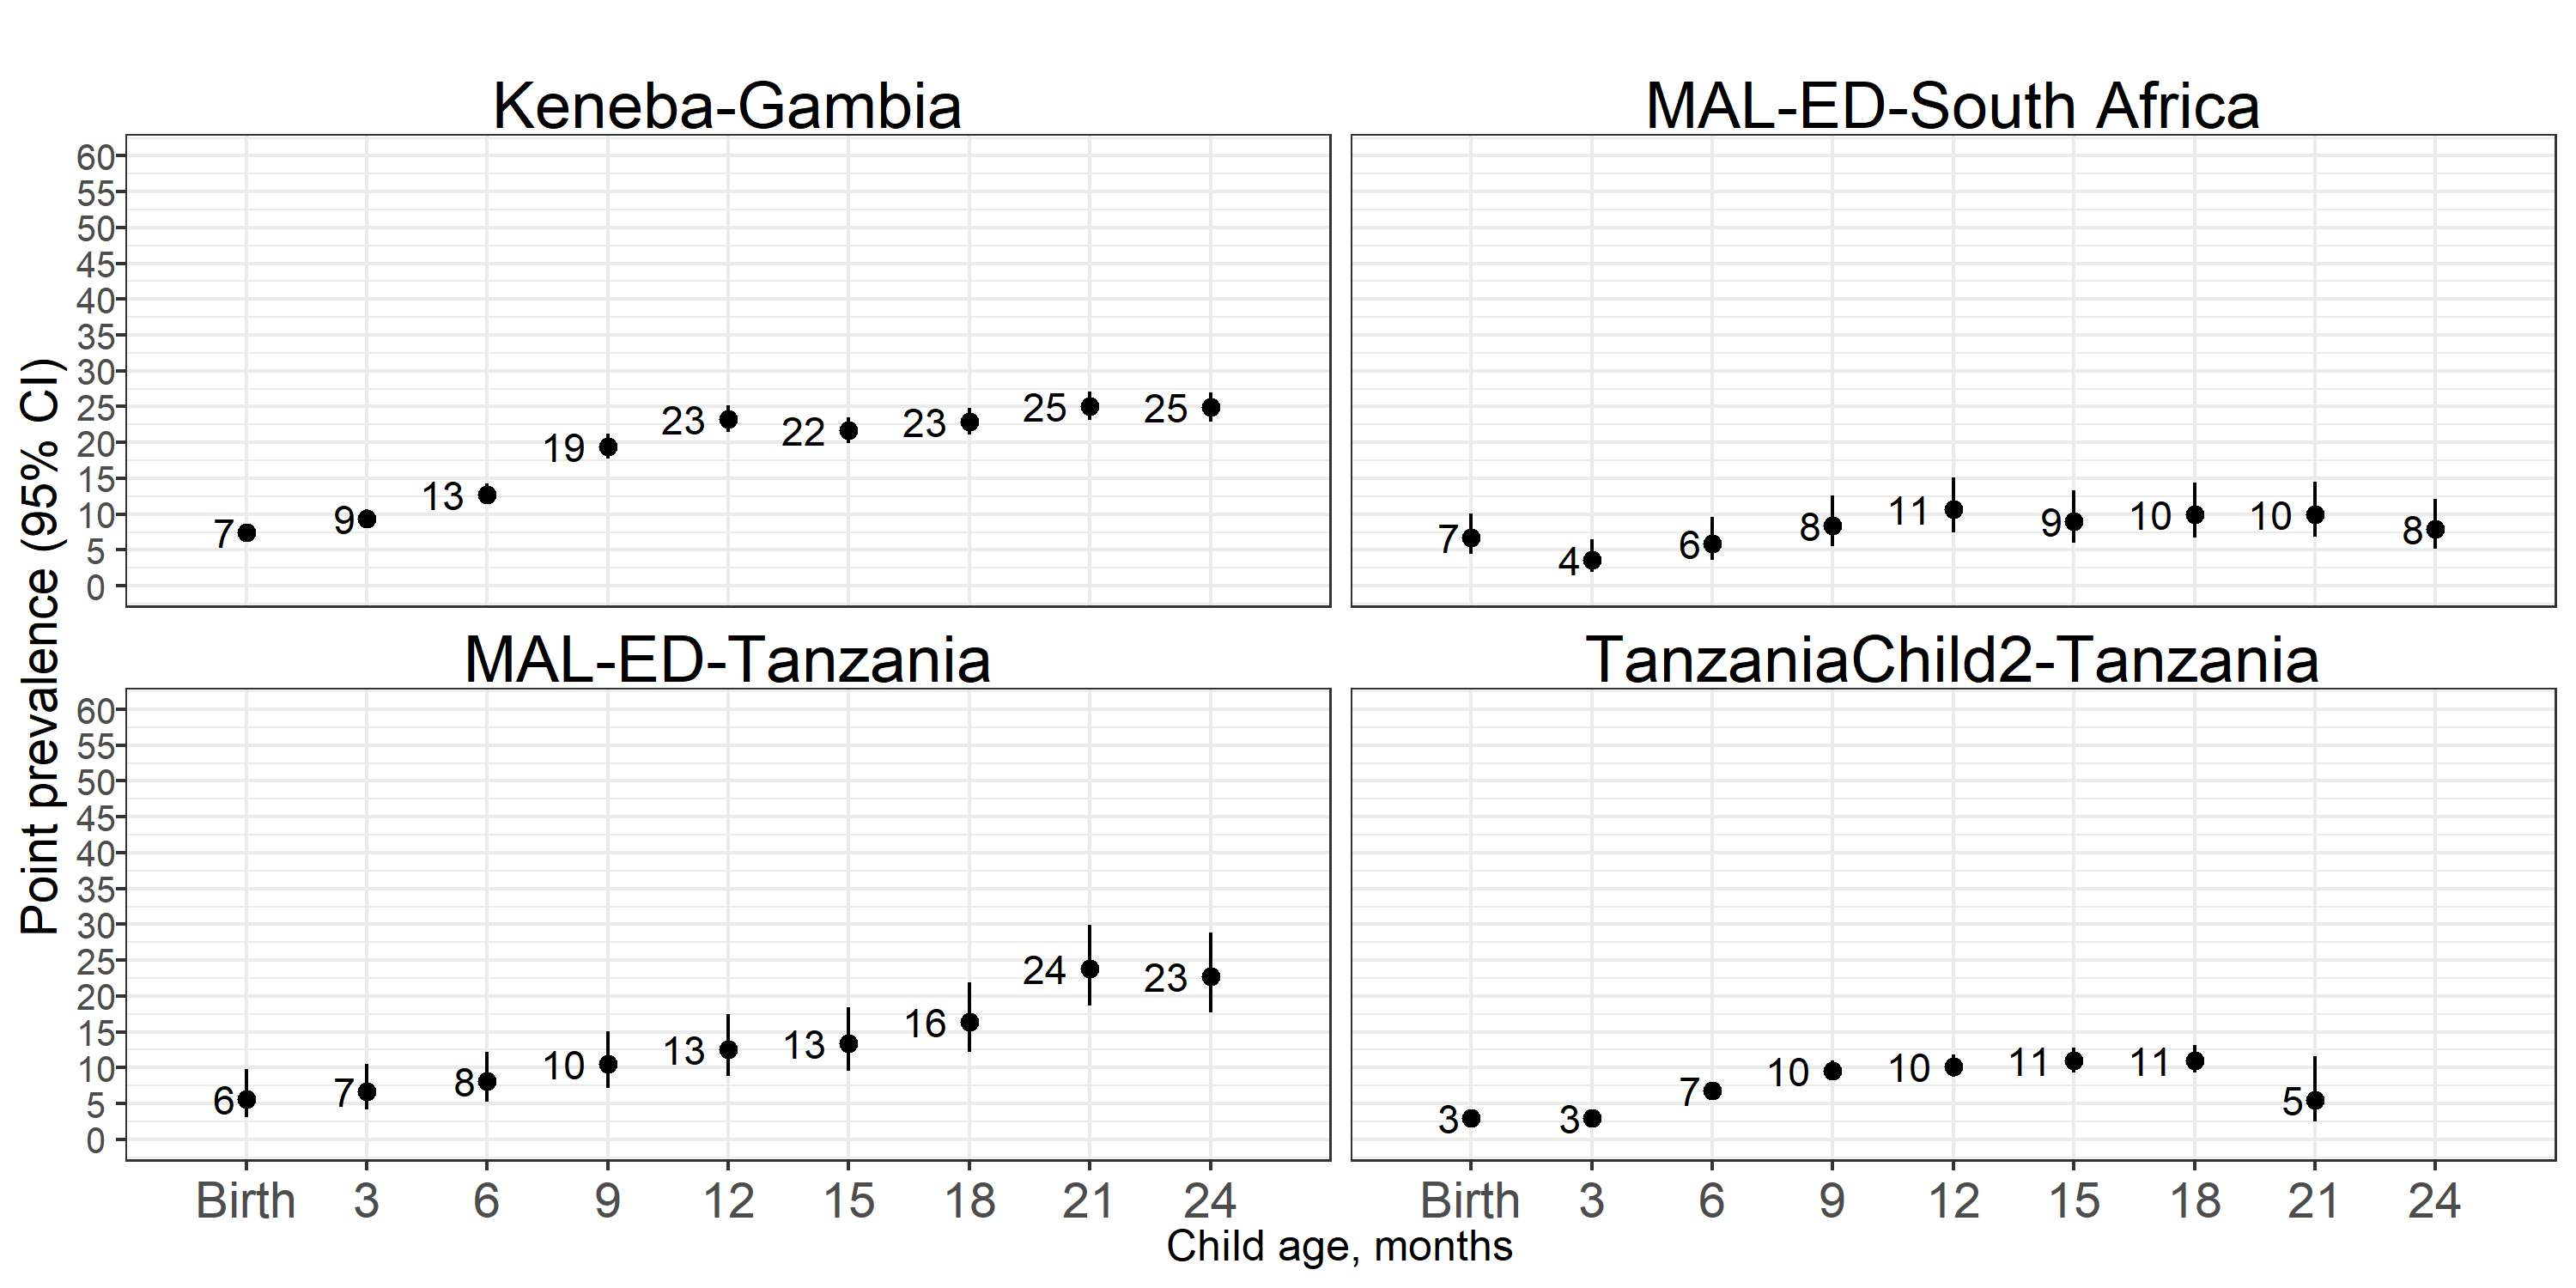
\includegraphics[width=41.67in]{C:/Users/andre/Documents/HBGDki/wasting/ki-longitudinal-manuscripts/figures/wasting/fig-underweight_plot_africa}
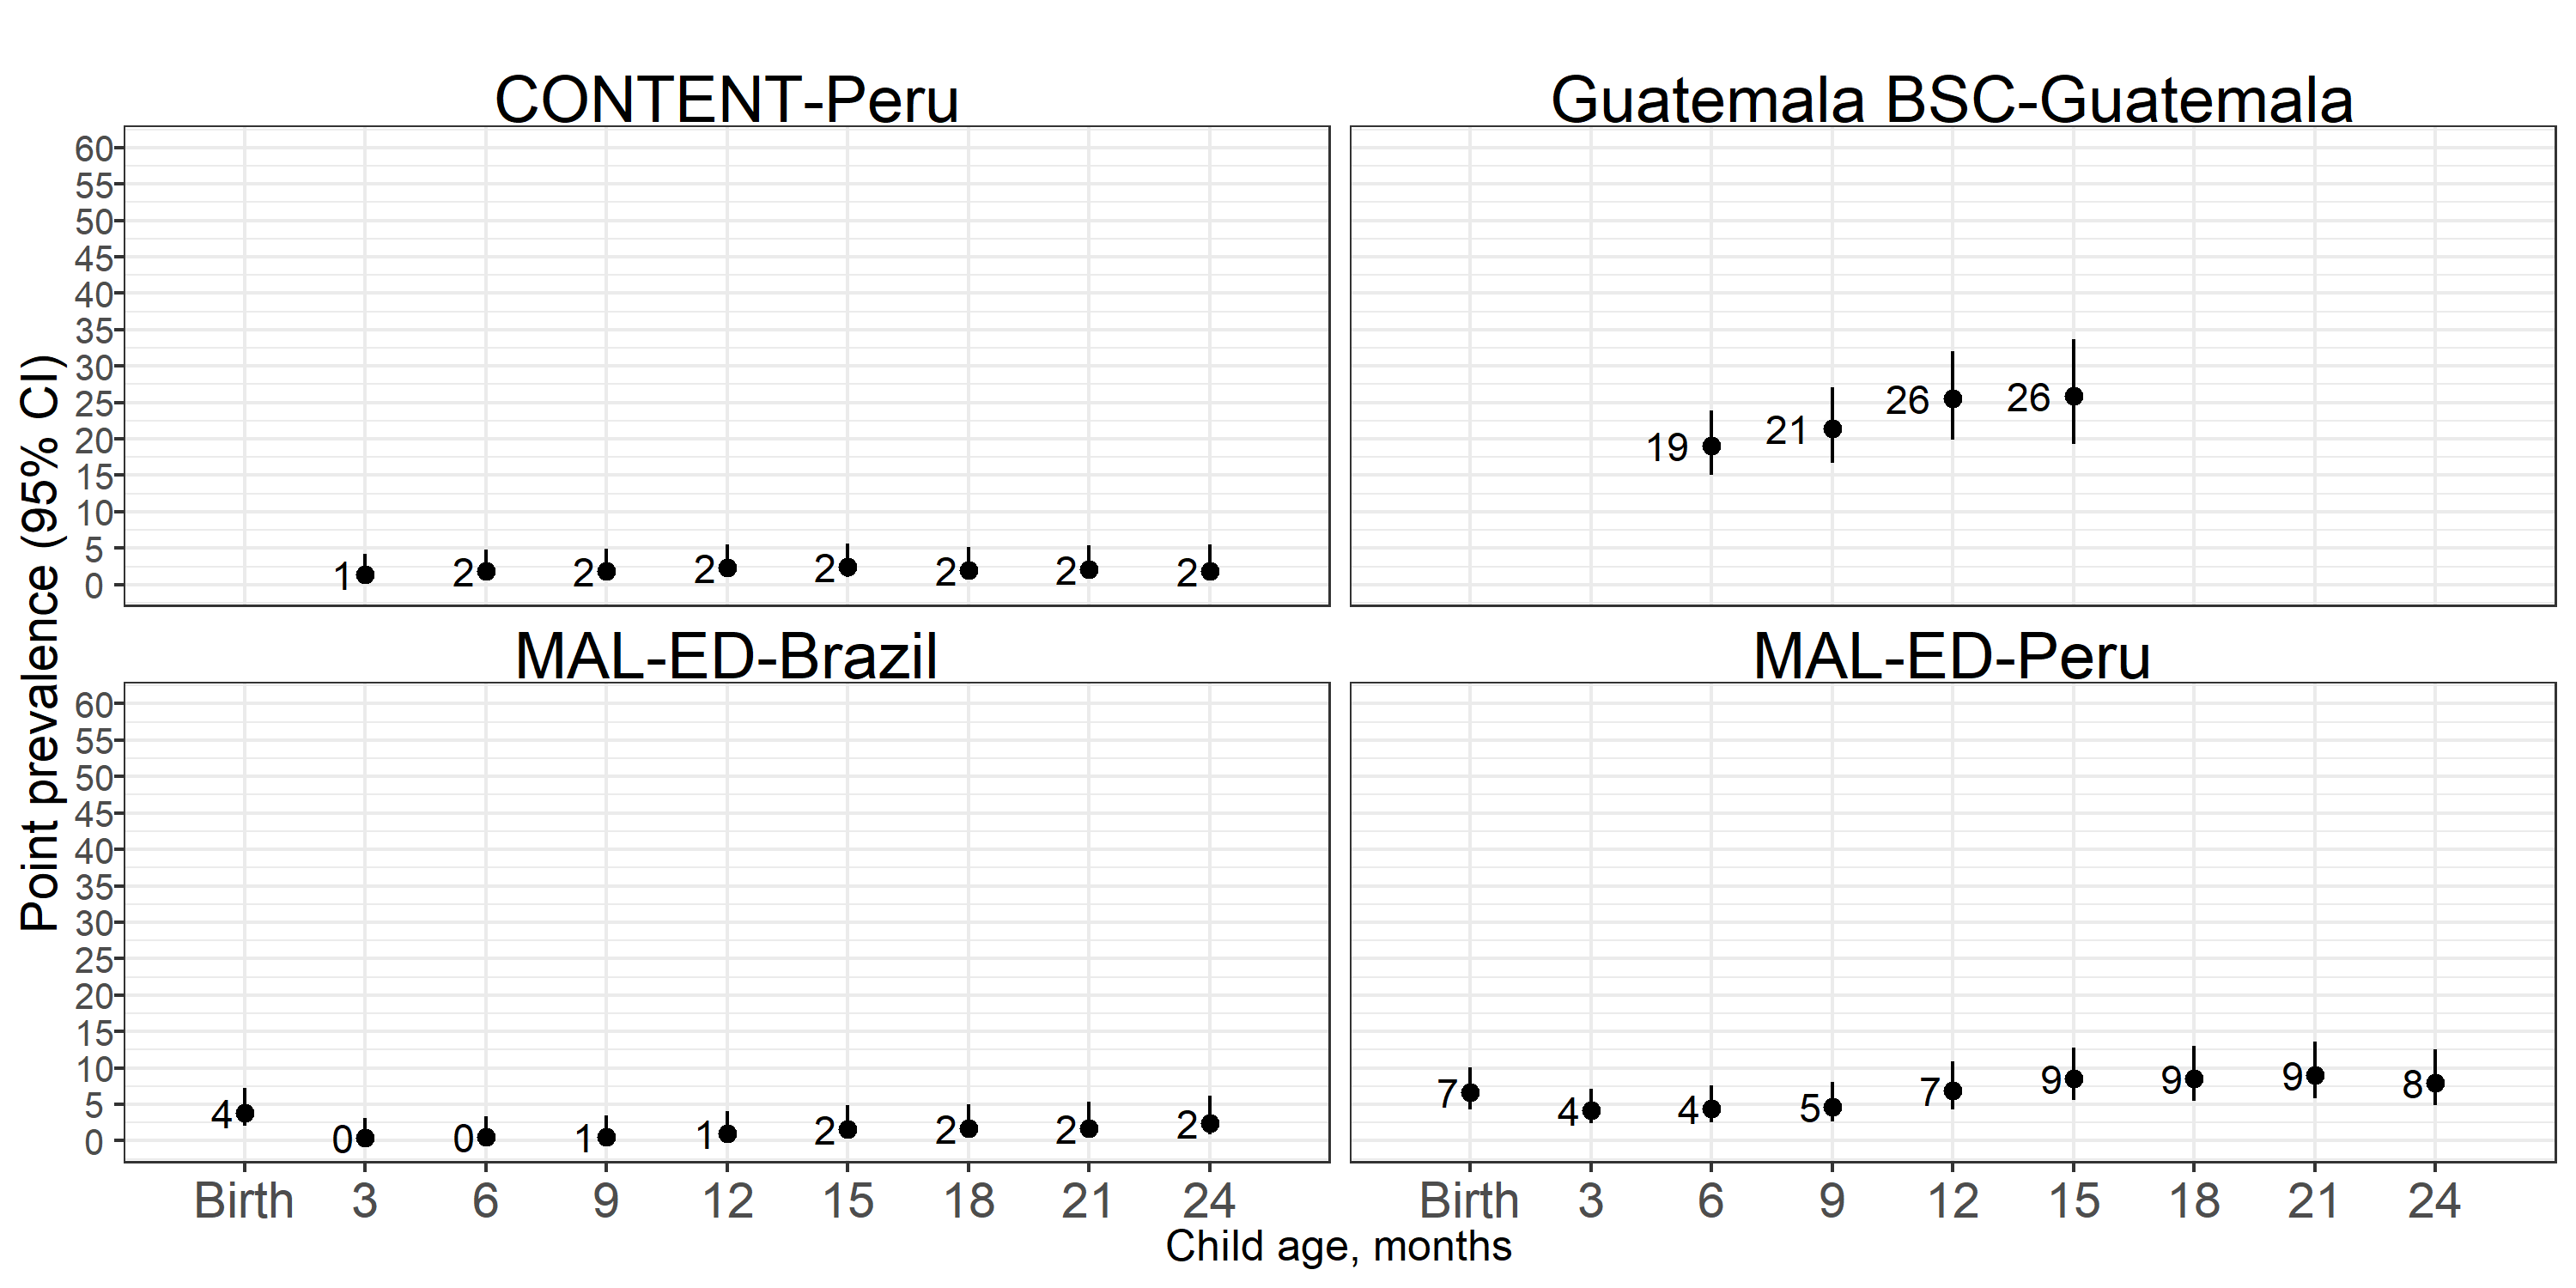
\includegraphics[width=41.67in]{C:/Users/andre/Documents/HBGDki/wasting/ki-longitudinal-manuscripts/figures/wasting/fig-underweight_plot_lam}
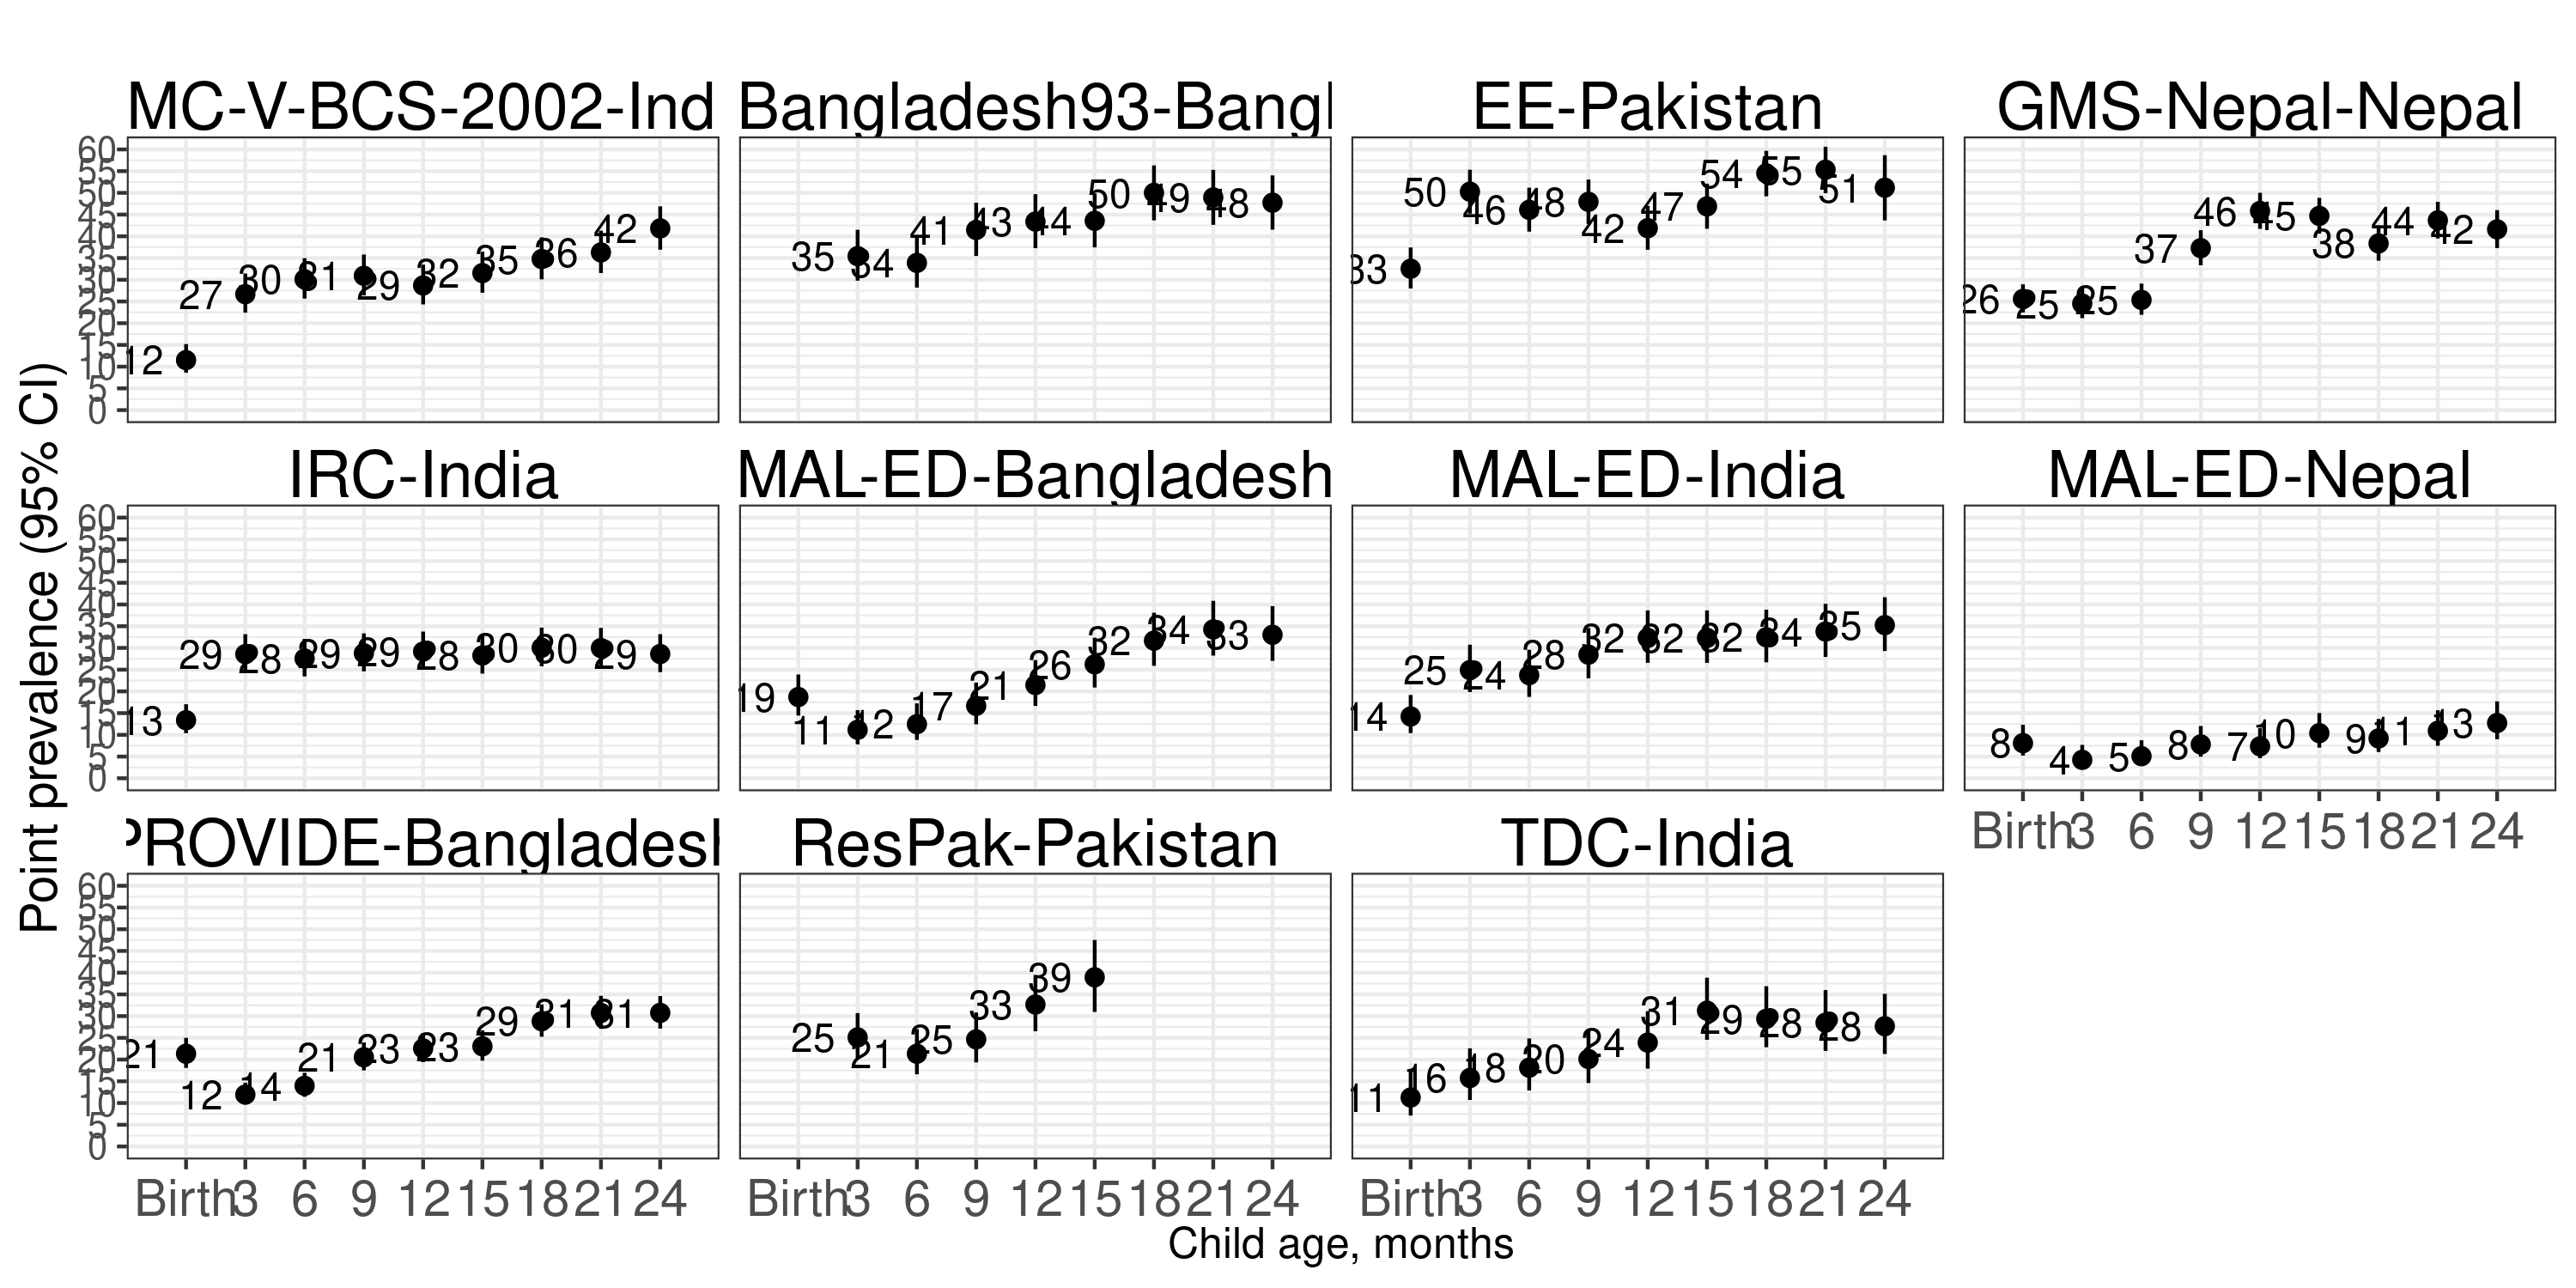
\includegraphics[width=41.67in]{C:/Users/andre/Documents/HBGDki/wasting/ki-longitudinal-manuscripts/figures/wasting/fig-underweight_plot_sasia}

\hypertarget{no-kenaba}{%
\chapter{Sensitivity analysis dropping at-Birth measures in Kenaba}\label{no-kenaba}}

\raggedright

Here, we re-estimate primary results after dropping the observations of children at birth within the MRC Kenaba cohort, which used a different team to measure child anthropometry at birth from the trained anthropometrists used in follow-up measurements. While other cohort data from the Kenaba area show that children tend to experience decreased LAZ after birth, in the MRC Kenaba data used in this analysis, we see a high birth LAZ (approximately 0) and a rapid drop in LAZ in followup measurements (approximately -1 at one month).
we see that the at birth measurements LAZ is \textasciitilde0, and then for the follow-up measurements after the mean LAZ is \textasciitilde{} -1 (and the mean LAZ of just the subsequent follow-up visit at one month is \textasciitilde{} -1). We calculated 30\% of measurements taken within two weeks of birth are lower than the at birth measurement beyond the technical error of measurement, and so are unrealistic decreases in child length, and 43\% of follow-up measurements within two weeks of birth are less than the at-birth measurement by any amount.

\hypertarget{mean-wlz-by-region}{%
\section{Mean WLZ by region}\label{mean-wlz-by-region}}

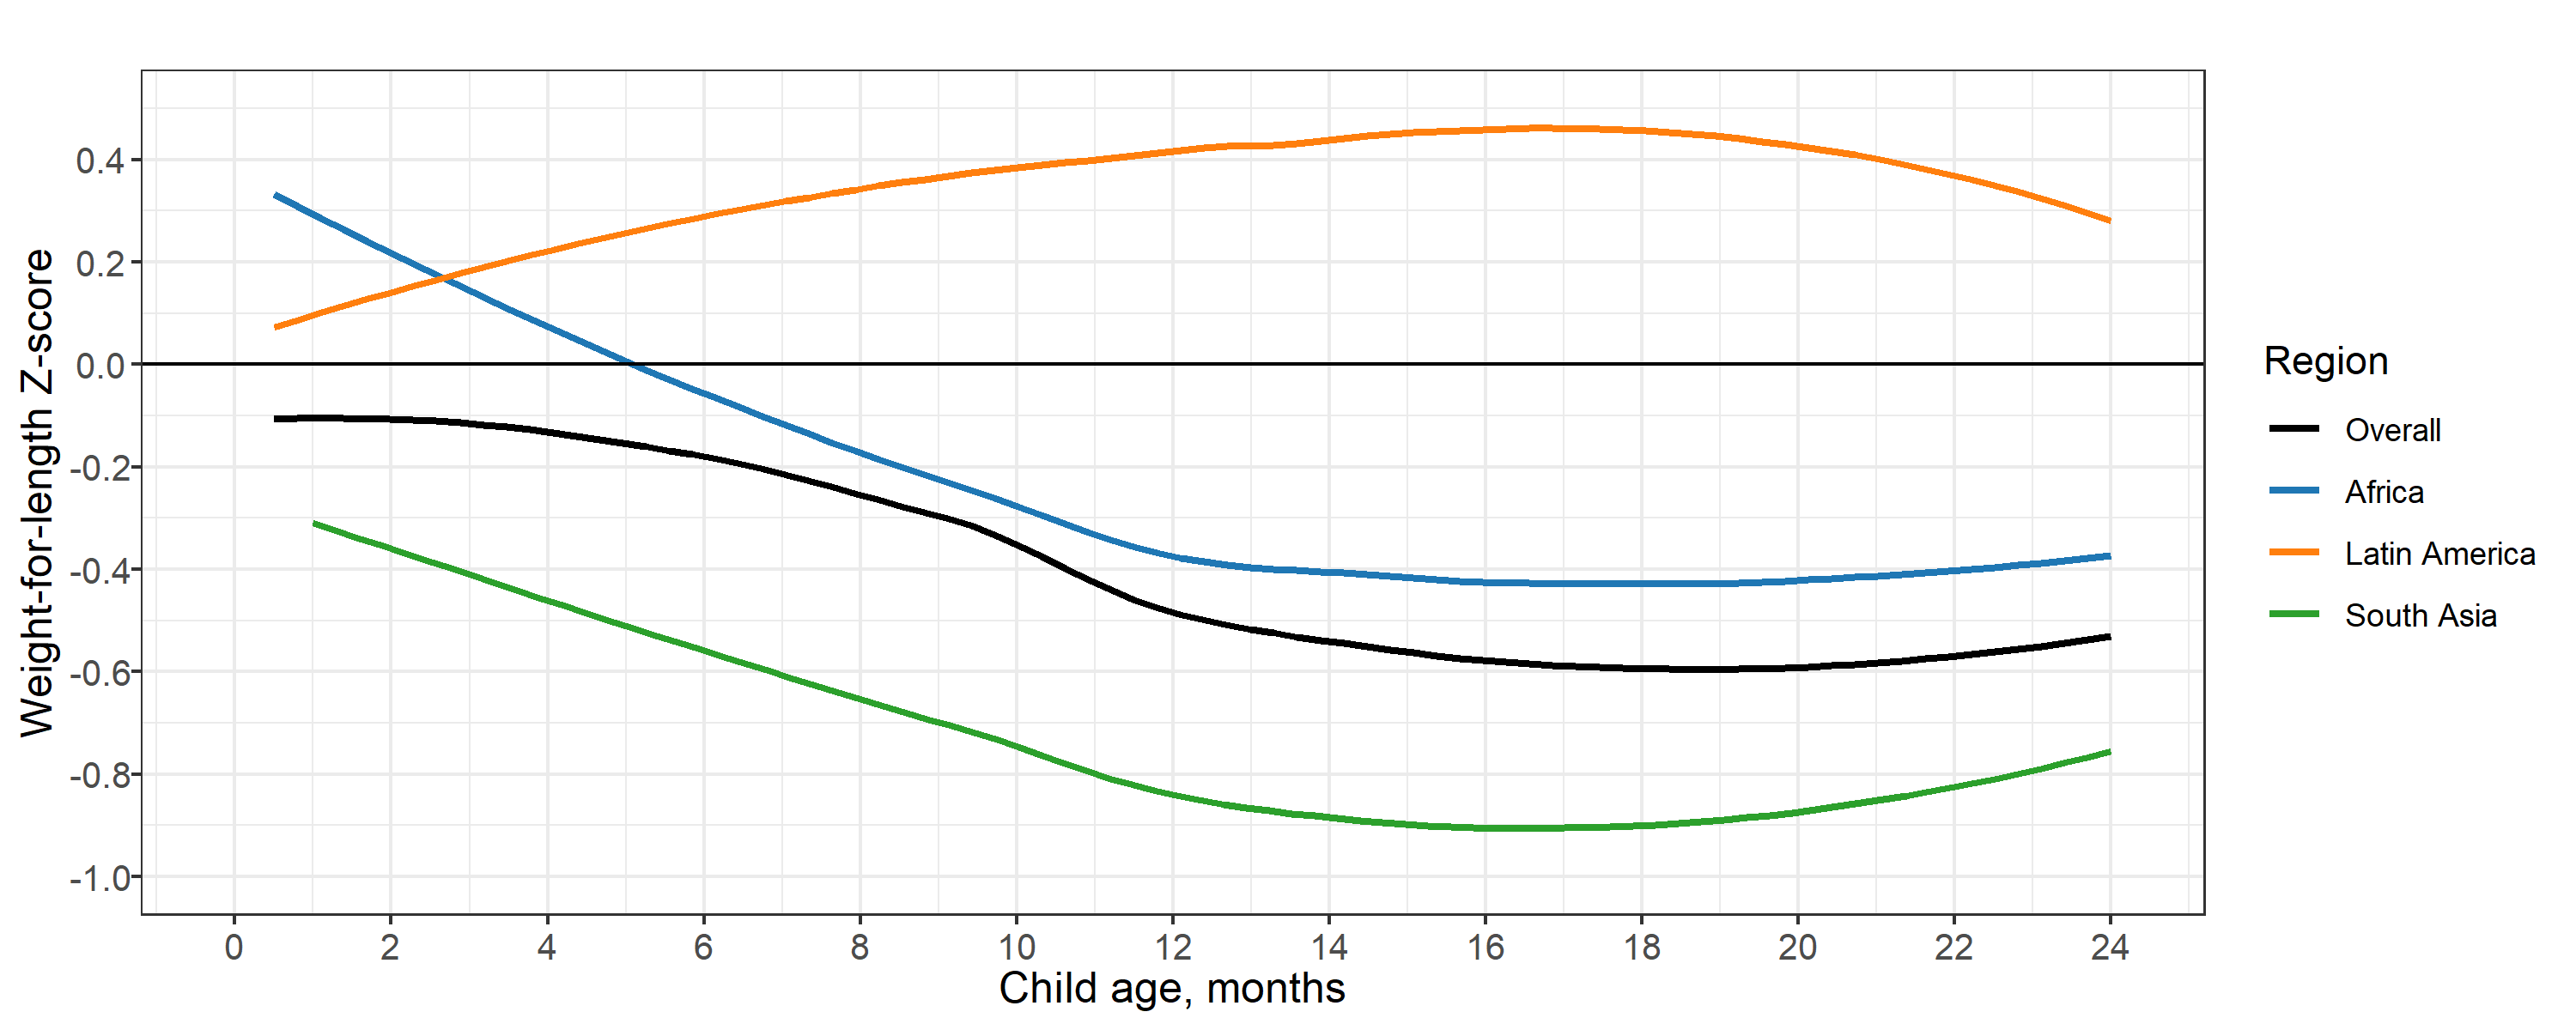
\includegraphics{C:/Users/andre/Documents/HBGDki/wasting/ki-longitudinal-manuscripts/figures/wasting/WLZ_by_region-no-Kenaba-BW.png}

\hypertarget{age-specific-prevalence-2}{%
\section{Age-specific prevalence}\label{age-specific-prevalence-2}}

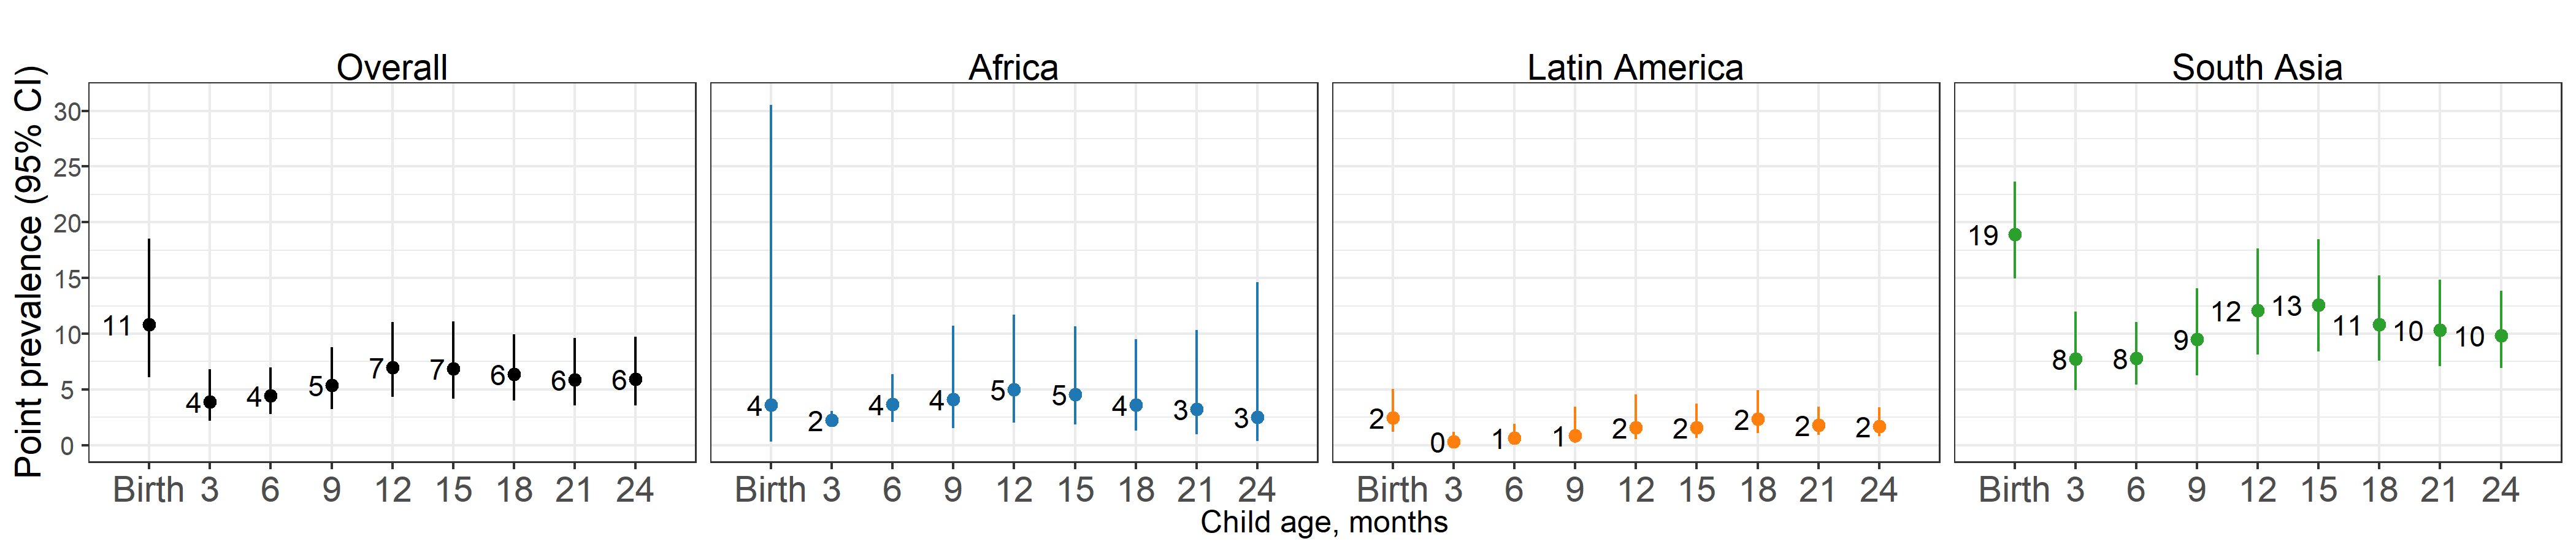
\includegraphics{C:/Users/andre/Documents/HBGDki/wasting/ki-longitudinal-manuscripts/figures/wasting/fig-wast-prev-no-Kenaba-BW.png}

\hypertarget{age-specific-incidence-1}{%
\section{Age-specific incidence}\label{age-specific-incidence-1}}

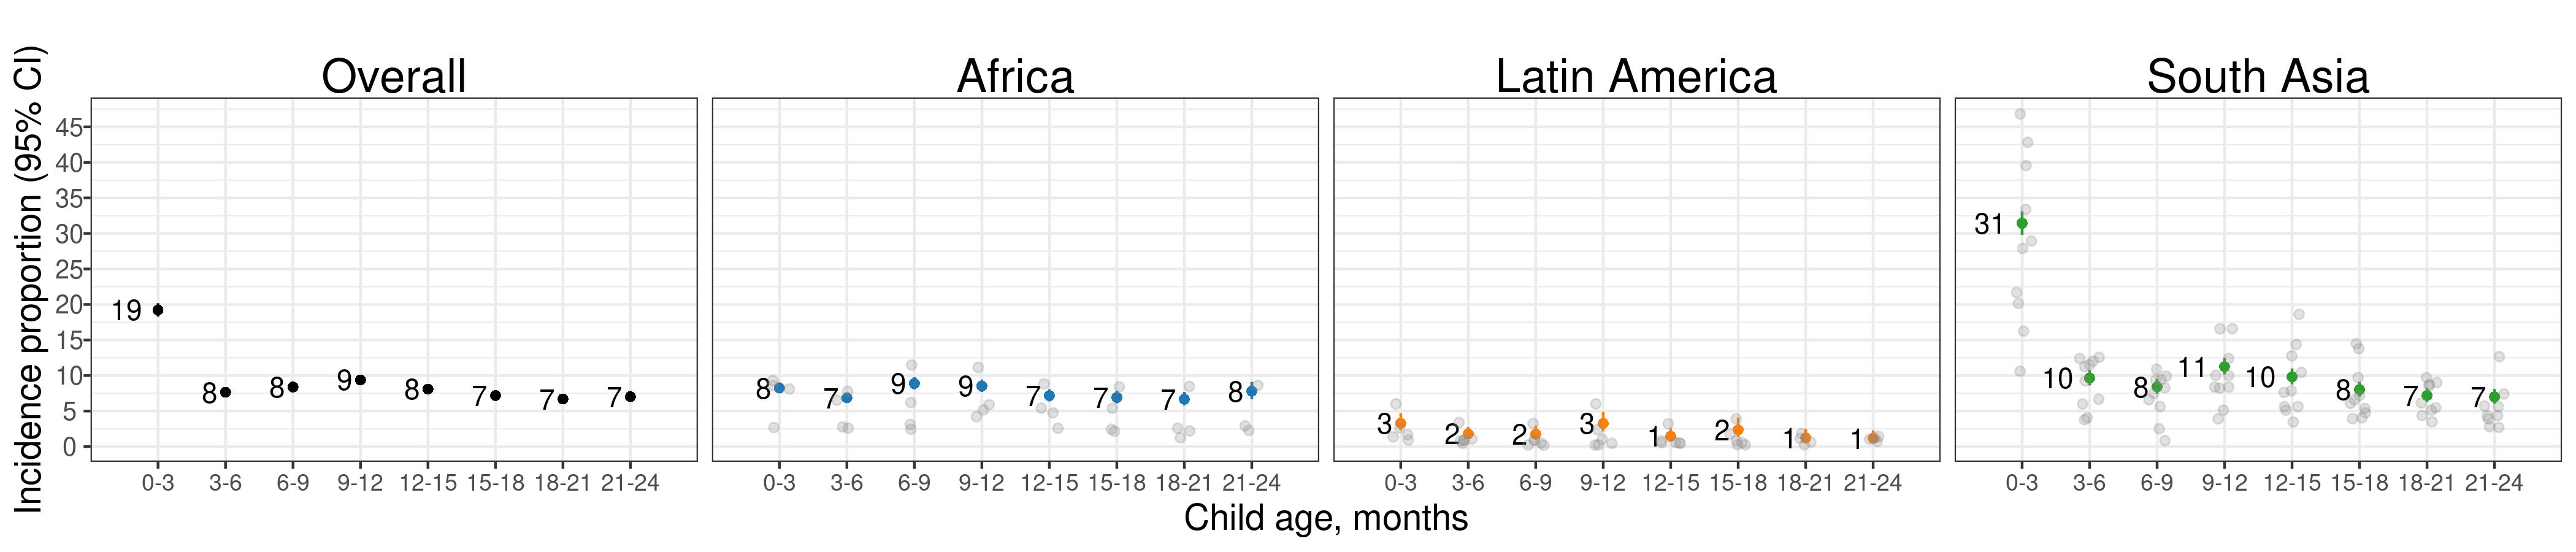
\includegraphics{C:/Users/andre/Documents/HBGDki/wasting/ki-longitudinal-manuscripts/figures/wasting/fig-wast-ci-no-Kenaba-BW.png}

\hypertarget{age-specific-incidence-rate-1}{%
\section{Age-specific incidence rate}\label{age-specific-incidence-rate-1}}

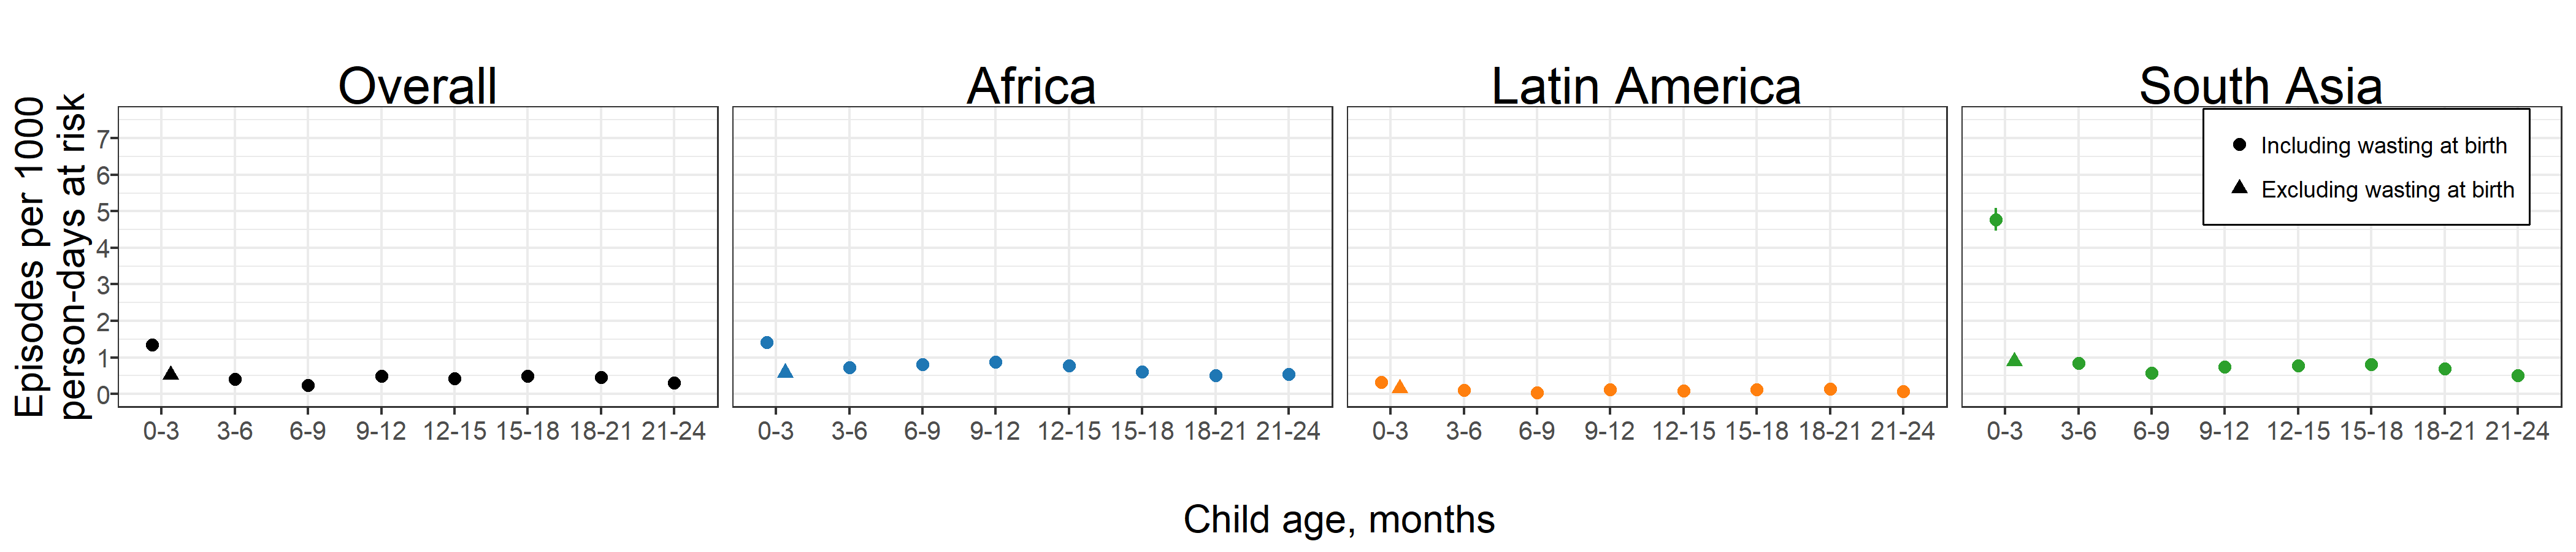
\includegraphics{C:/Users/andre/Documents/HBGDki/wasting/ki-longitudinal-manuscripts/figures/wasting/fig-wast-ir-no-Kenaba-BW.png}

\hypertarget{age-specific-recovery-1}{%
\section{Age-specific recovery}\label{age-specific-recovery-1}}

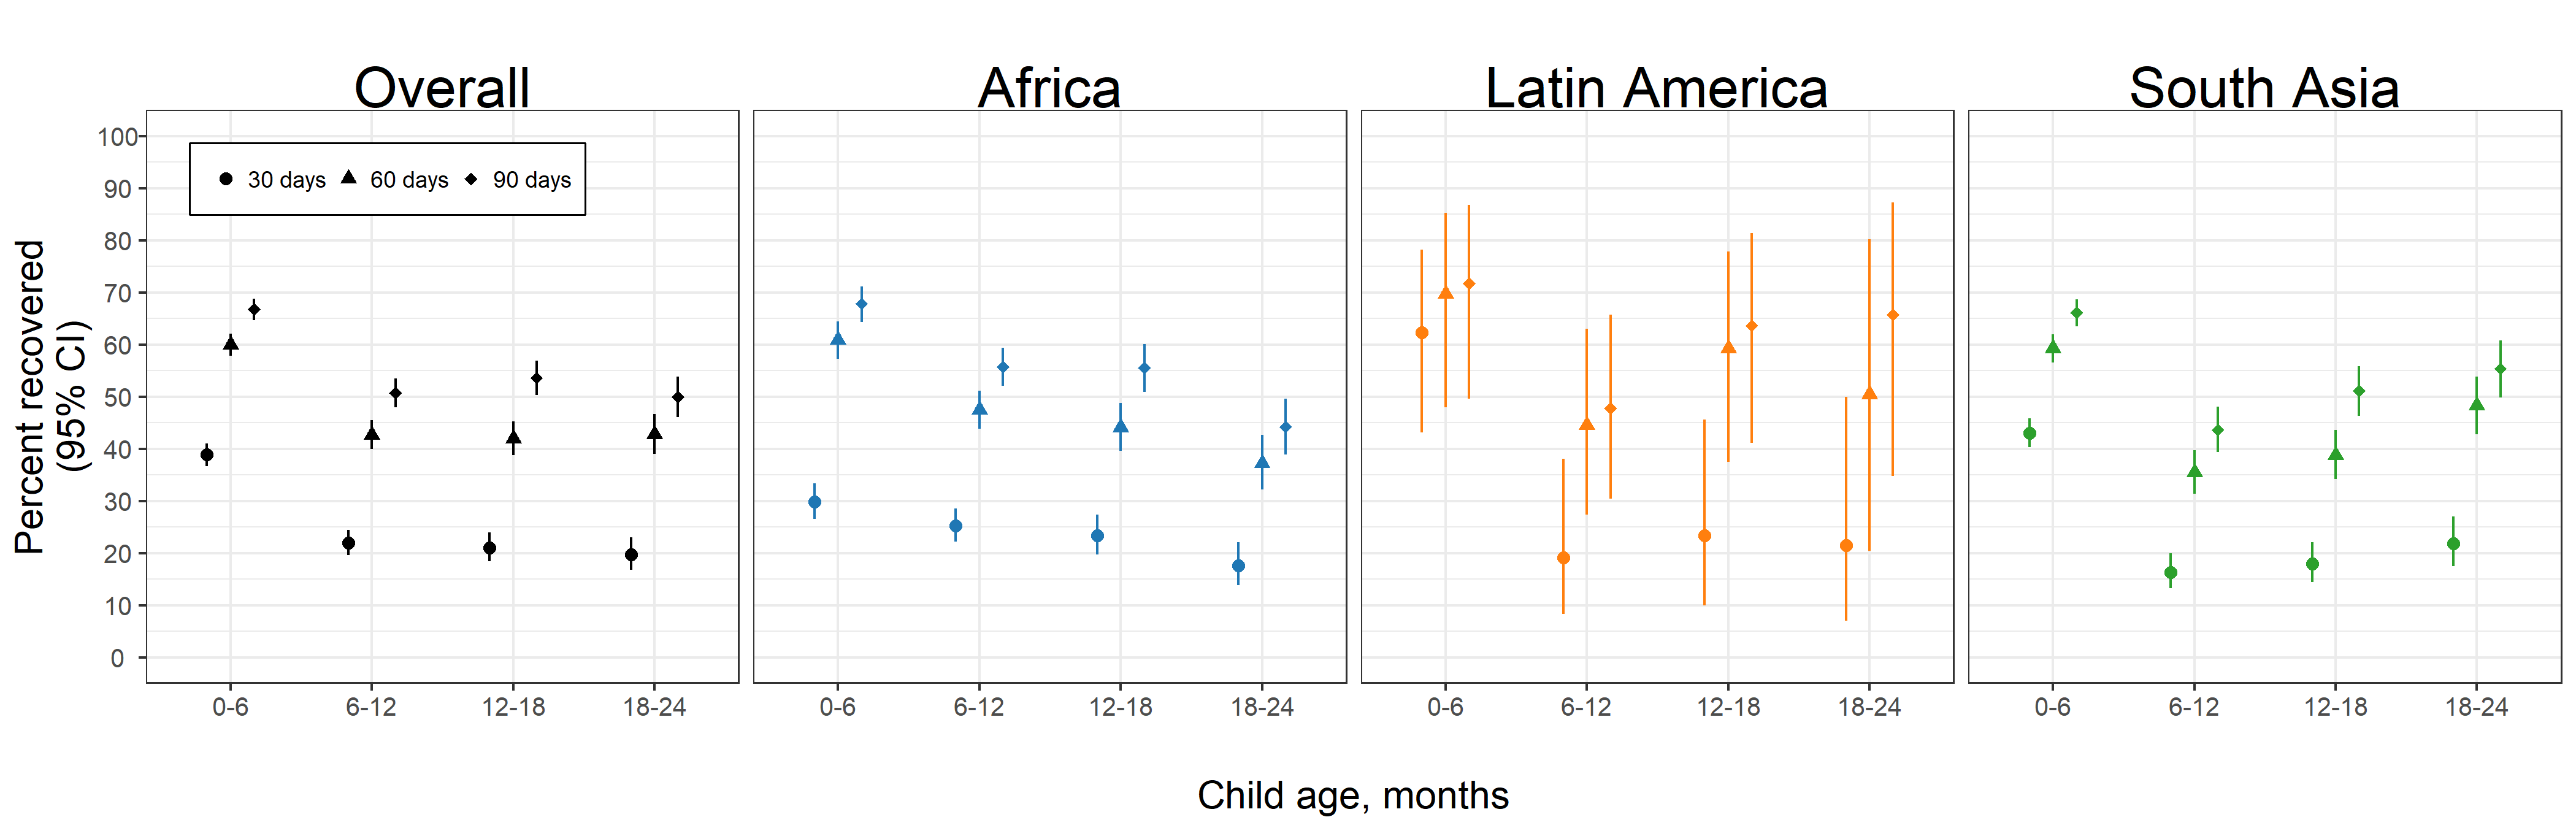
\includegraphics{C:/Users/andre/Documents/HBGDki/wasting/ki-longitudinal-manuscripts/figures/wasting/fig-wast-rec-no-Kenaba-BW.png}

\hypertarget{age-specific-prevalence-of-severe-wasting-2}{%
\section{Age-specific prevalence of severe wasting}\label{age-specific-prevalence-of-severe-wasting-2}}

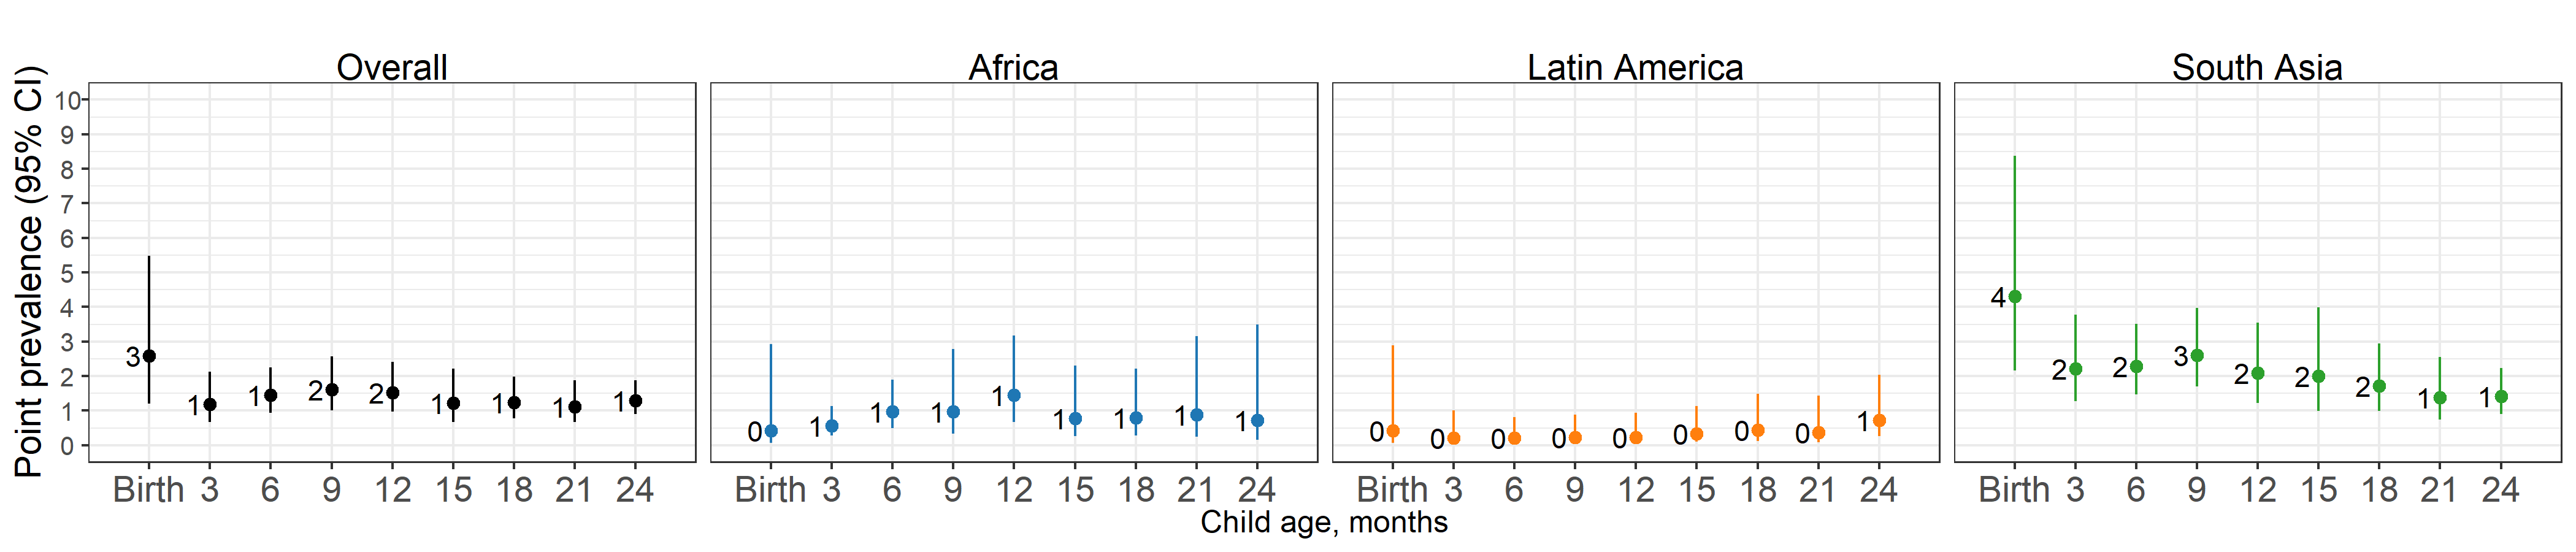
\includegraphics{C:/Users/andre/Documents/HBGDki/wasting/ki-longitudinal-manuscripts/figures/wasting/fig-sev-wast-no-Kenaba-BW.png}

\hypertarget{age-specific-longitudinal-prevalence-of-persistent-wasting-2}{%
\section{Age-specific longitudinal prevalence of persistent wasting}\label{age-specific-longitudinal-prevalence-of-persistent-wasting-2}}

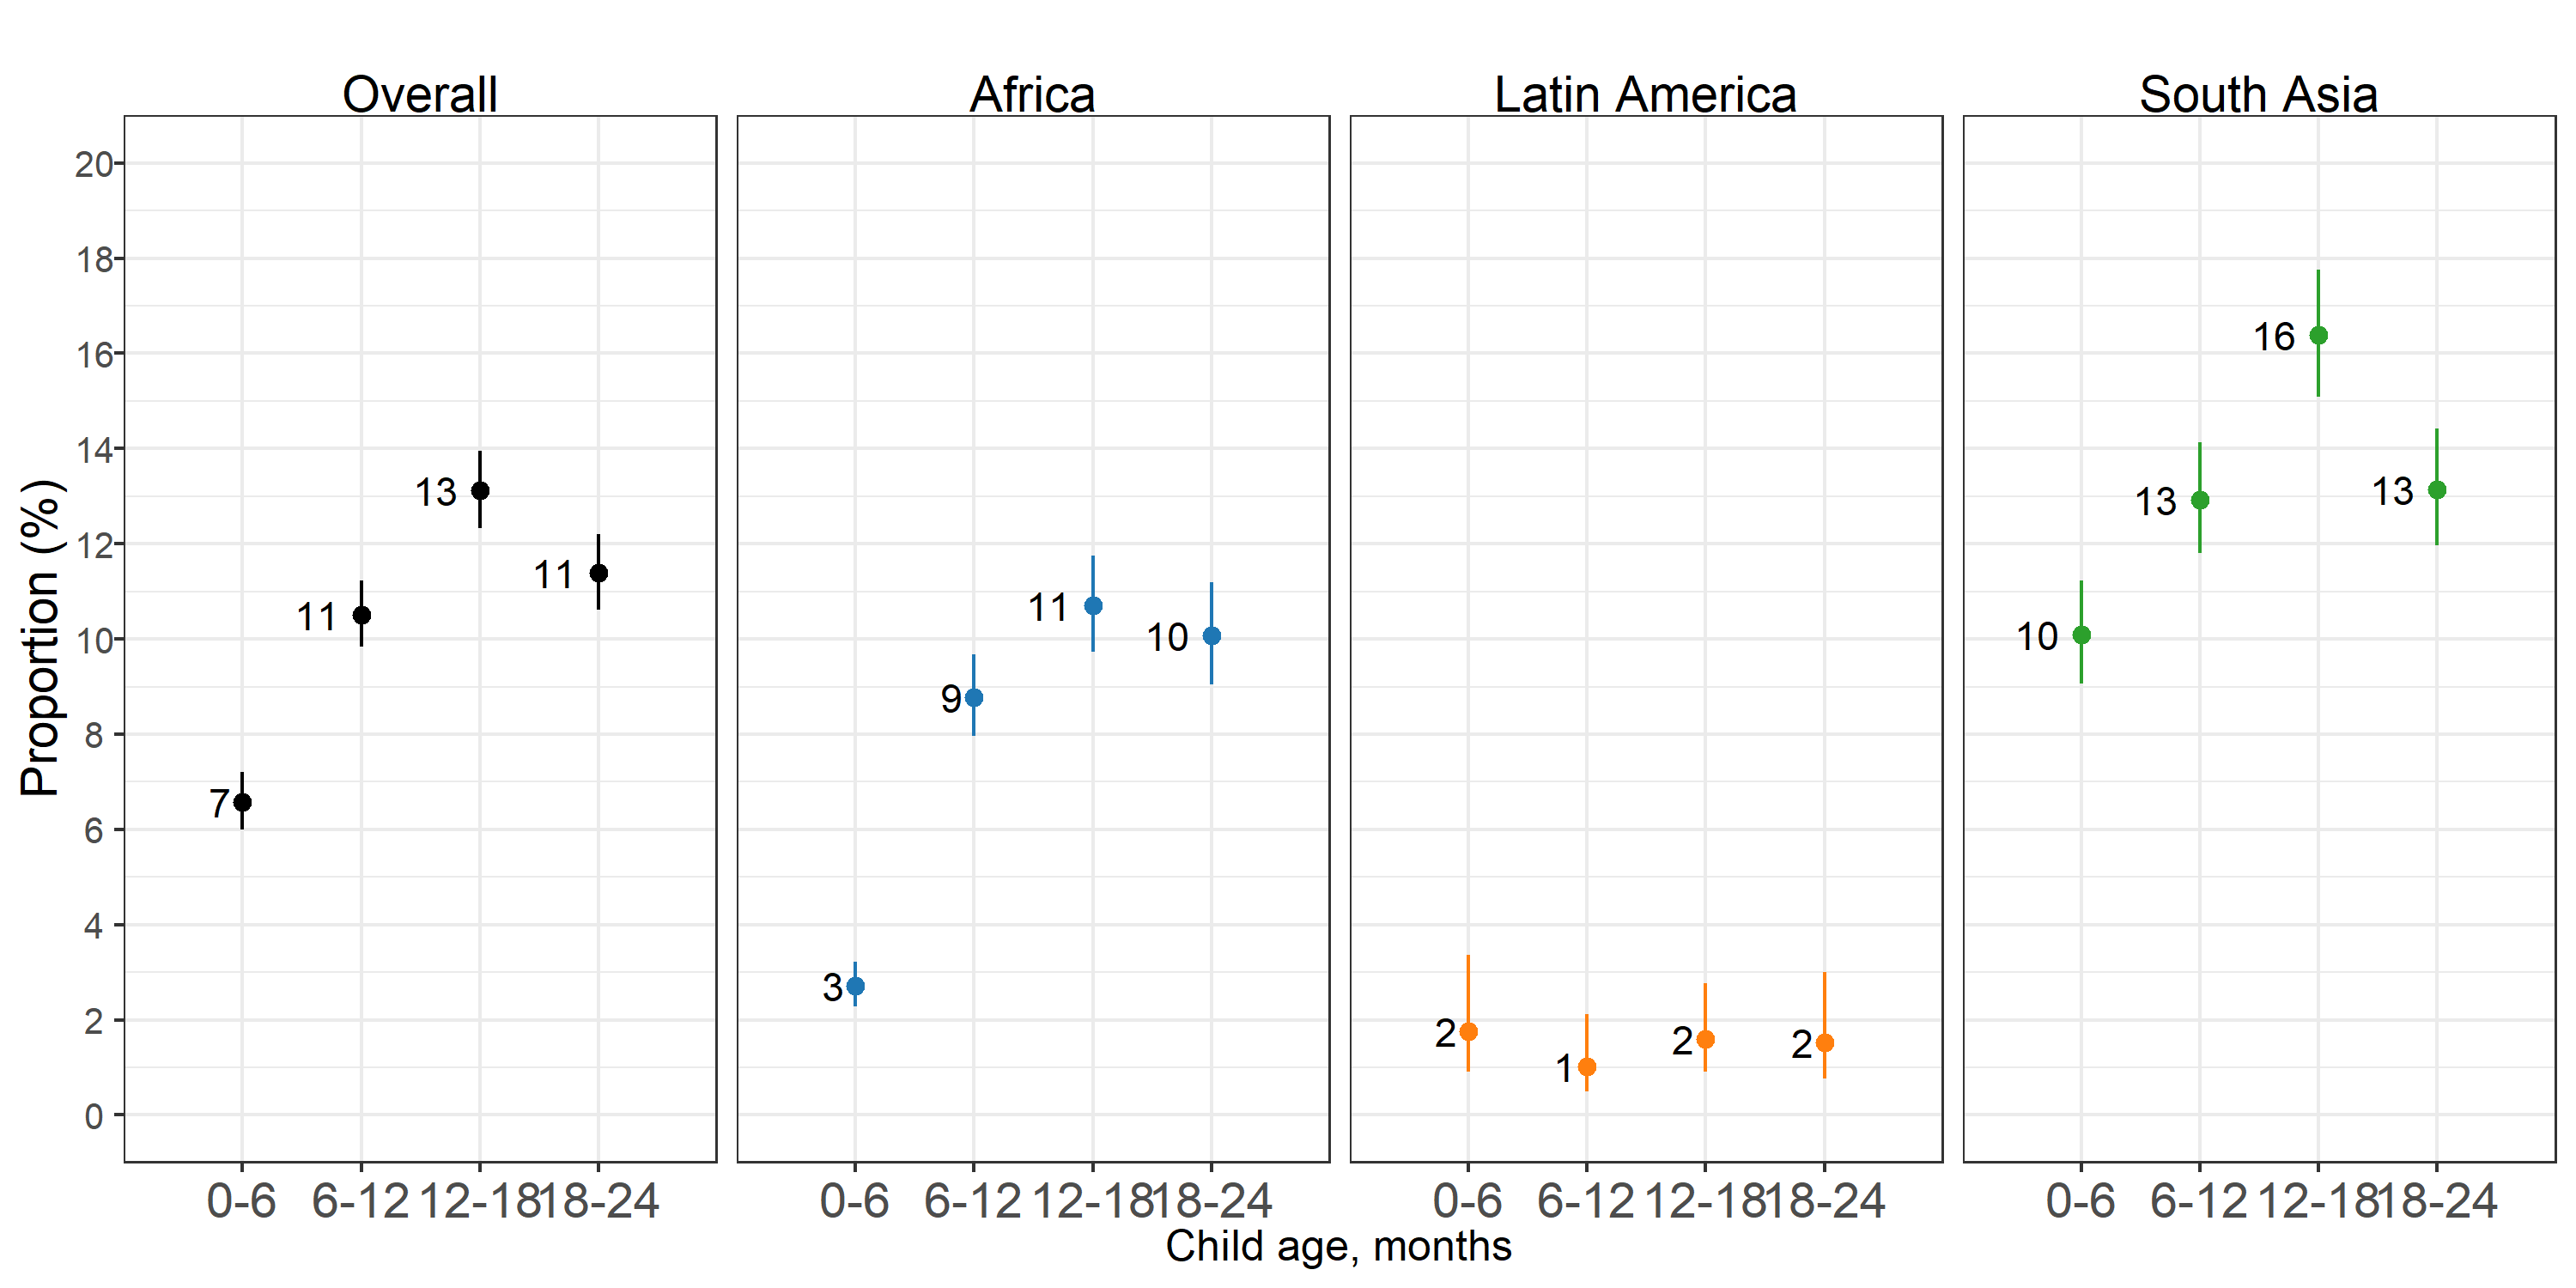
\includegraphics{C:/Users/andre/Documents/HBGDki/wasting/ki-longitudinal-manuscripts/figures/wasting/fig-pers-wast-no-Kenaba-BW.png}

\hypertarget{age-specific-prevalence-of-concurrent-wasting-and-stunting-2}{%
\section{Age-specific prevalence of concurrent wasting and stunting}\label{age-specific-prevalence-of-concurrent-wasting-and-stunting-2}}

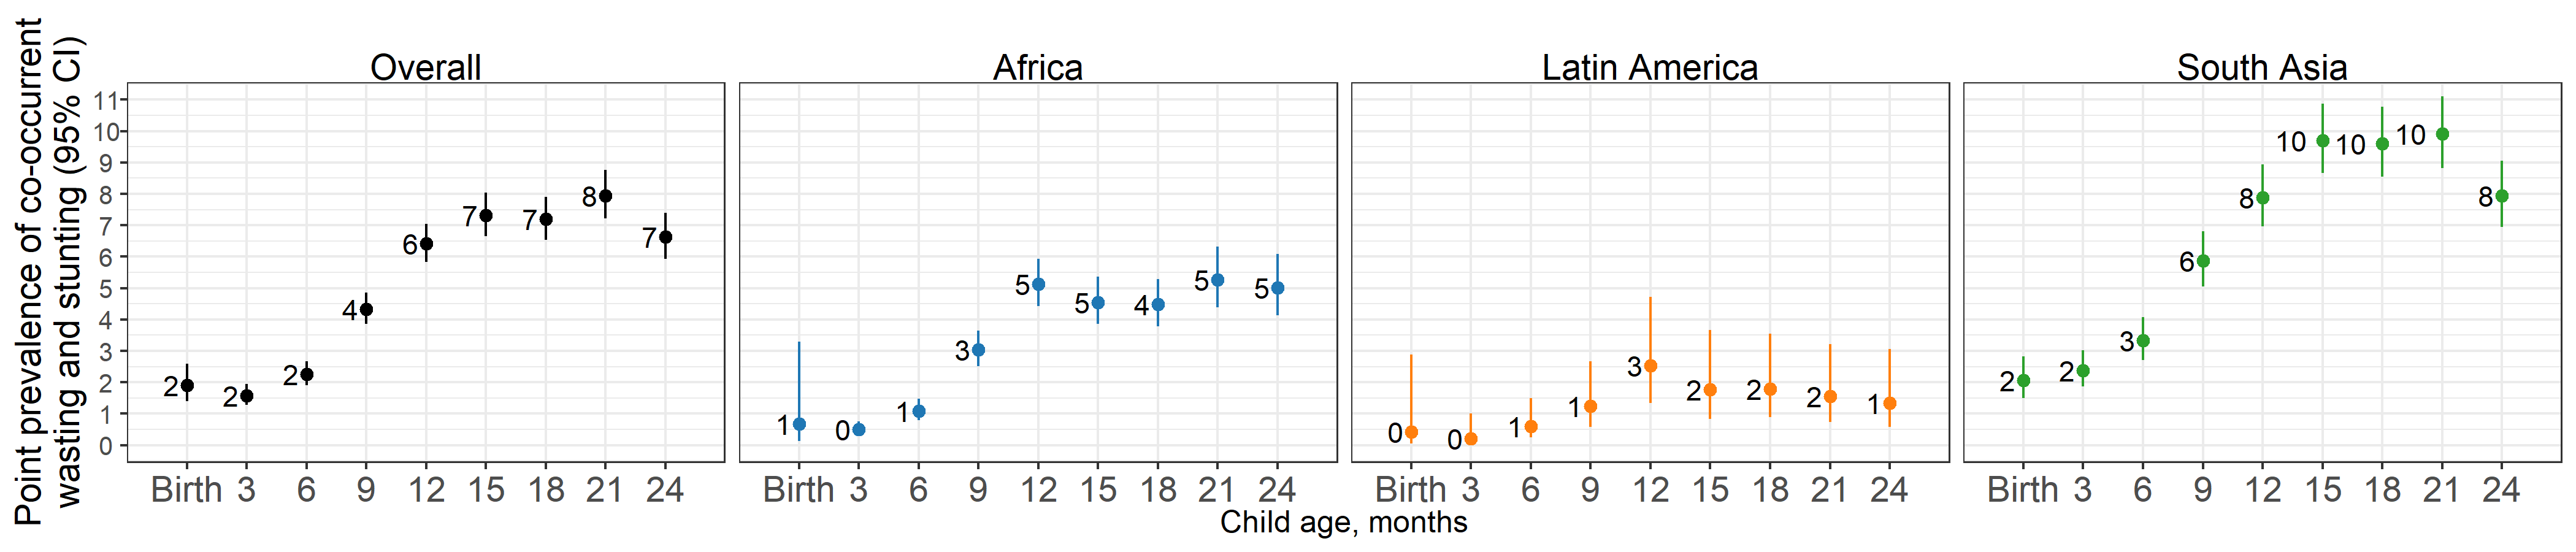
\includegraphics{C:/Users/andre/Documents/HBGDki/wasting/ki-longitudinal-manuscripts/figures/wasting/fig-co-prev-no-Kenaba-BW.png}

\hypertarget{age-specific-prevalence-of-underweight-weight-for-age-z-score--2-1}{%
\section{Age-specific prevalence of underweight (weight-for-age Z-score \textless{} -2)}\label{age-specific-prevalence-of-underweight-weight-for-age-z-score--2-1}}

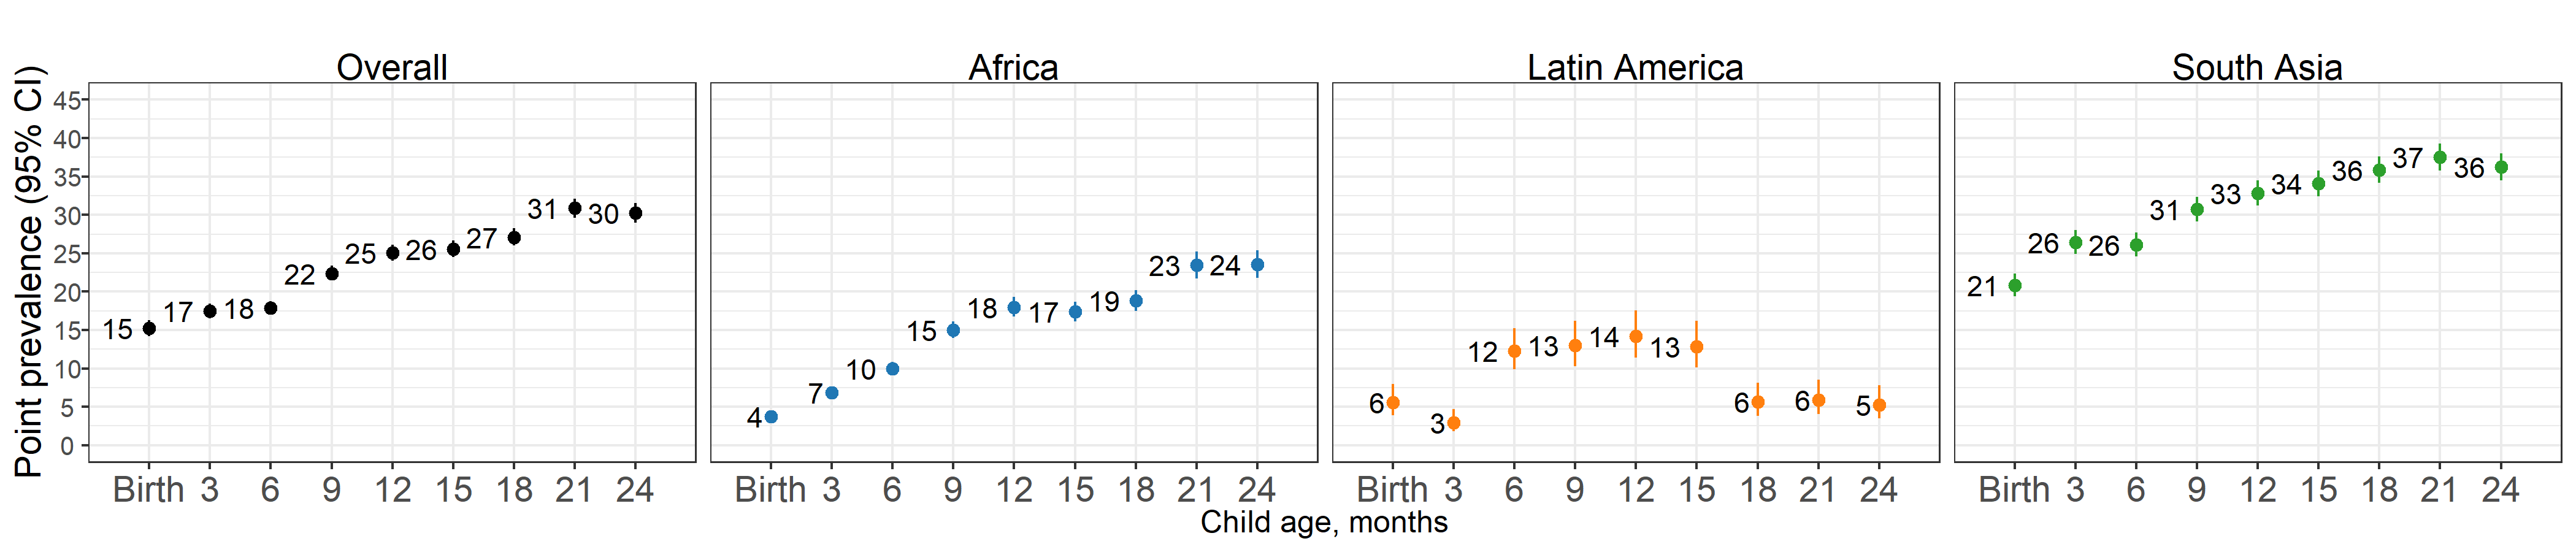
\includegraphics{C:/Users/andre/Documents/HBGDki/wasting/ki-longitudinal-manuscripts/figures/wasting/fig-uw-prev-no-Kenaba-BW.png}

\hypertarget{muac}{%
\chapter{Sensitivity analysis comparing wasting defined via weight-for-length versus middle-upper arm circumference}\label{muac}}

\raggedright

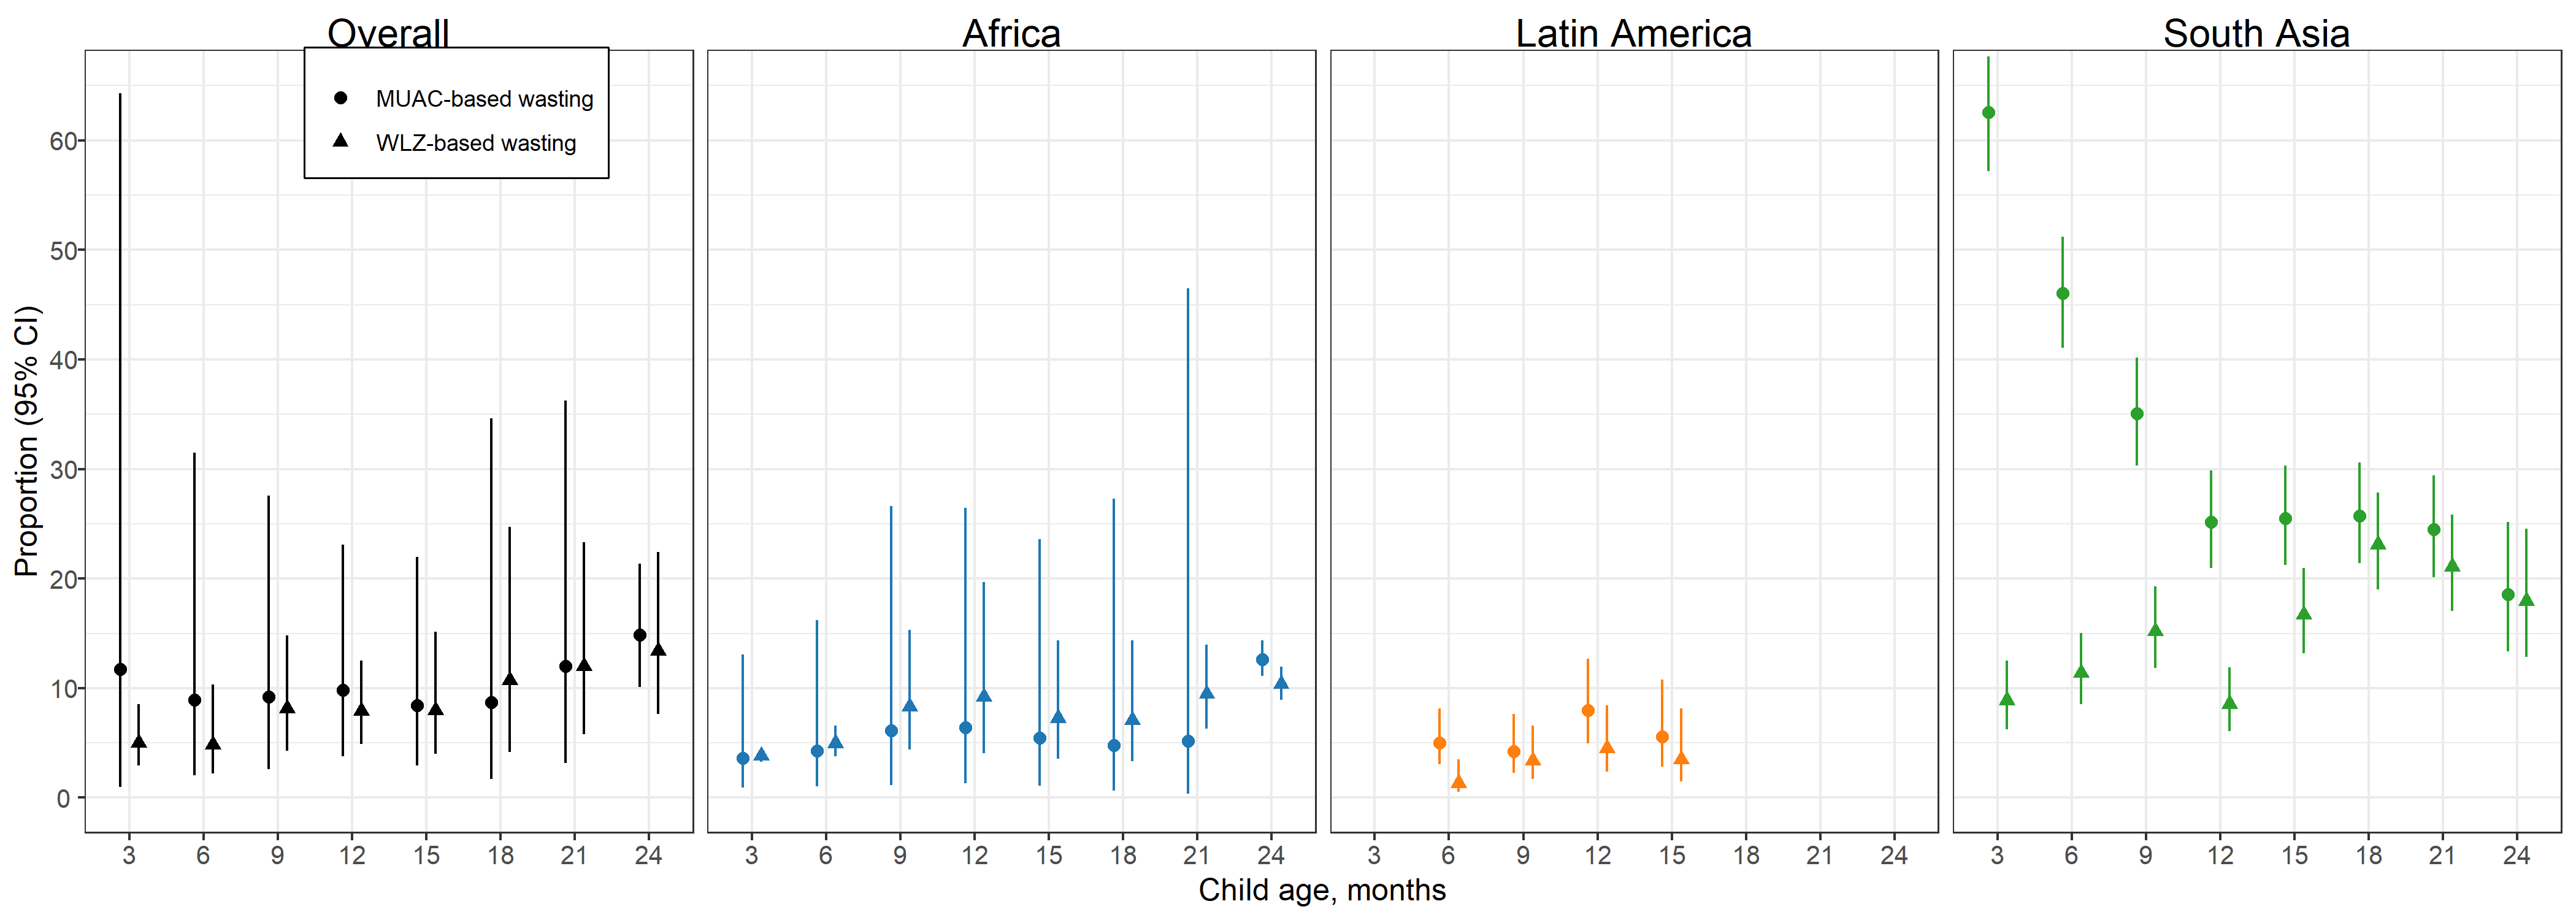
\includegraphics[width=58.33in]{C:/Users/andre/Documents/HBGDki/wasting/ki-longitudinal-manuscripts/figures/wasting/fig-wast-2-muac-overall_region--allage-primary}

\hypertarget{anthro}{%
\chapter{Anthropometry measurement quality}\label{anthro}}

\raggedright

\hypertarget{anthropometry-measuresments-compared-to-who-standards}{%
\section{Anthropometry measuresments compared to WHO standards}\label{anthropometry-measuresments-compared-to-who-standards}}

To check for outliers in length measurements, We plotted the distribution of raw length and weight measurements by age and sex against bands marking the first, second, and third standard deviations of the World Health Organization child growth standard distribution. The majority of observations fell within 3 standard deviations of the mean of the standard for males and females.

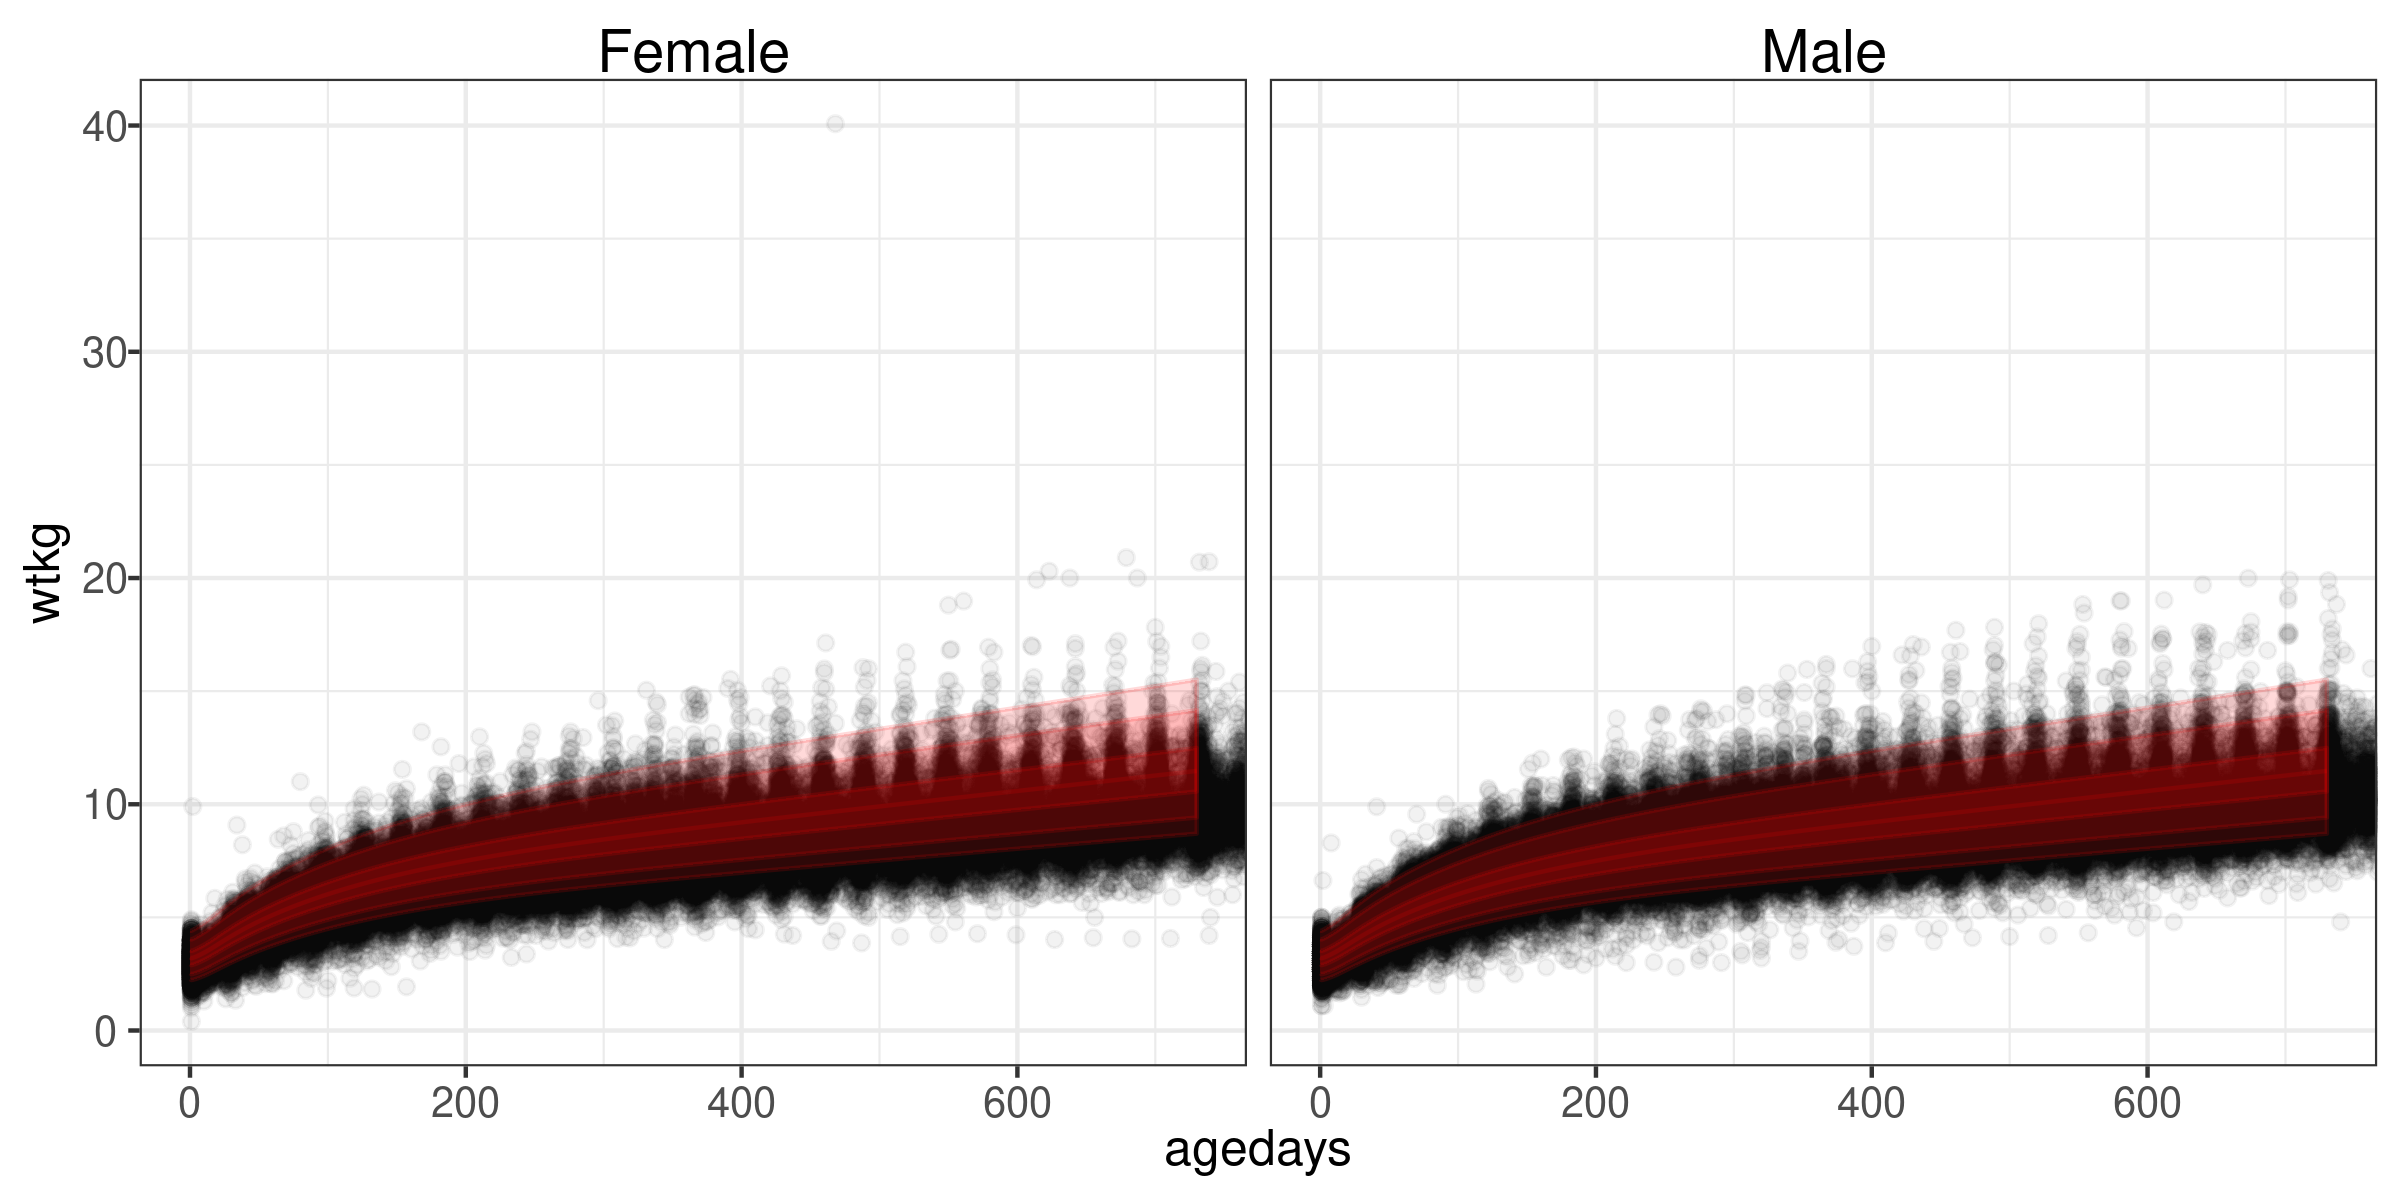
\includegraphics[width=33.33in]{C:/Users/andre/Documents/HBGDki/wasting/ki-longitudinal-manuscripts/figures/shared/waz_QA_monthly}
\includegraphics[width=104.17in]{C:/Users/andre/Documents/HBGDki/wasting/ki-longitudinal-manuscripts/figures/shared/waz_QA_cohort_monthly}
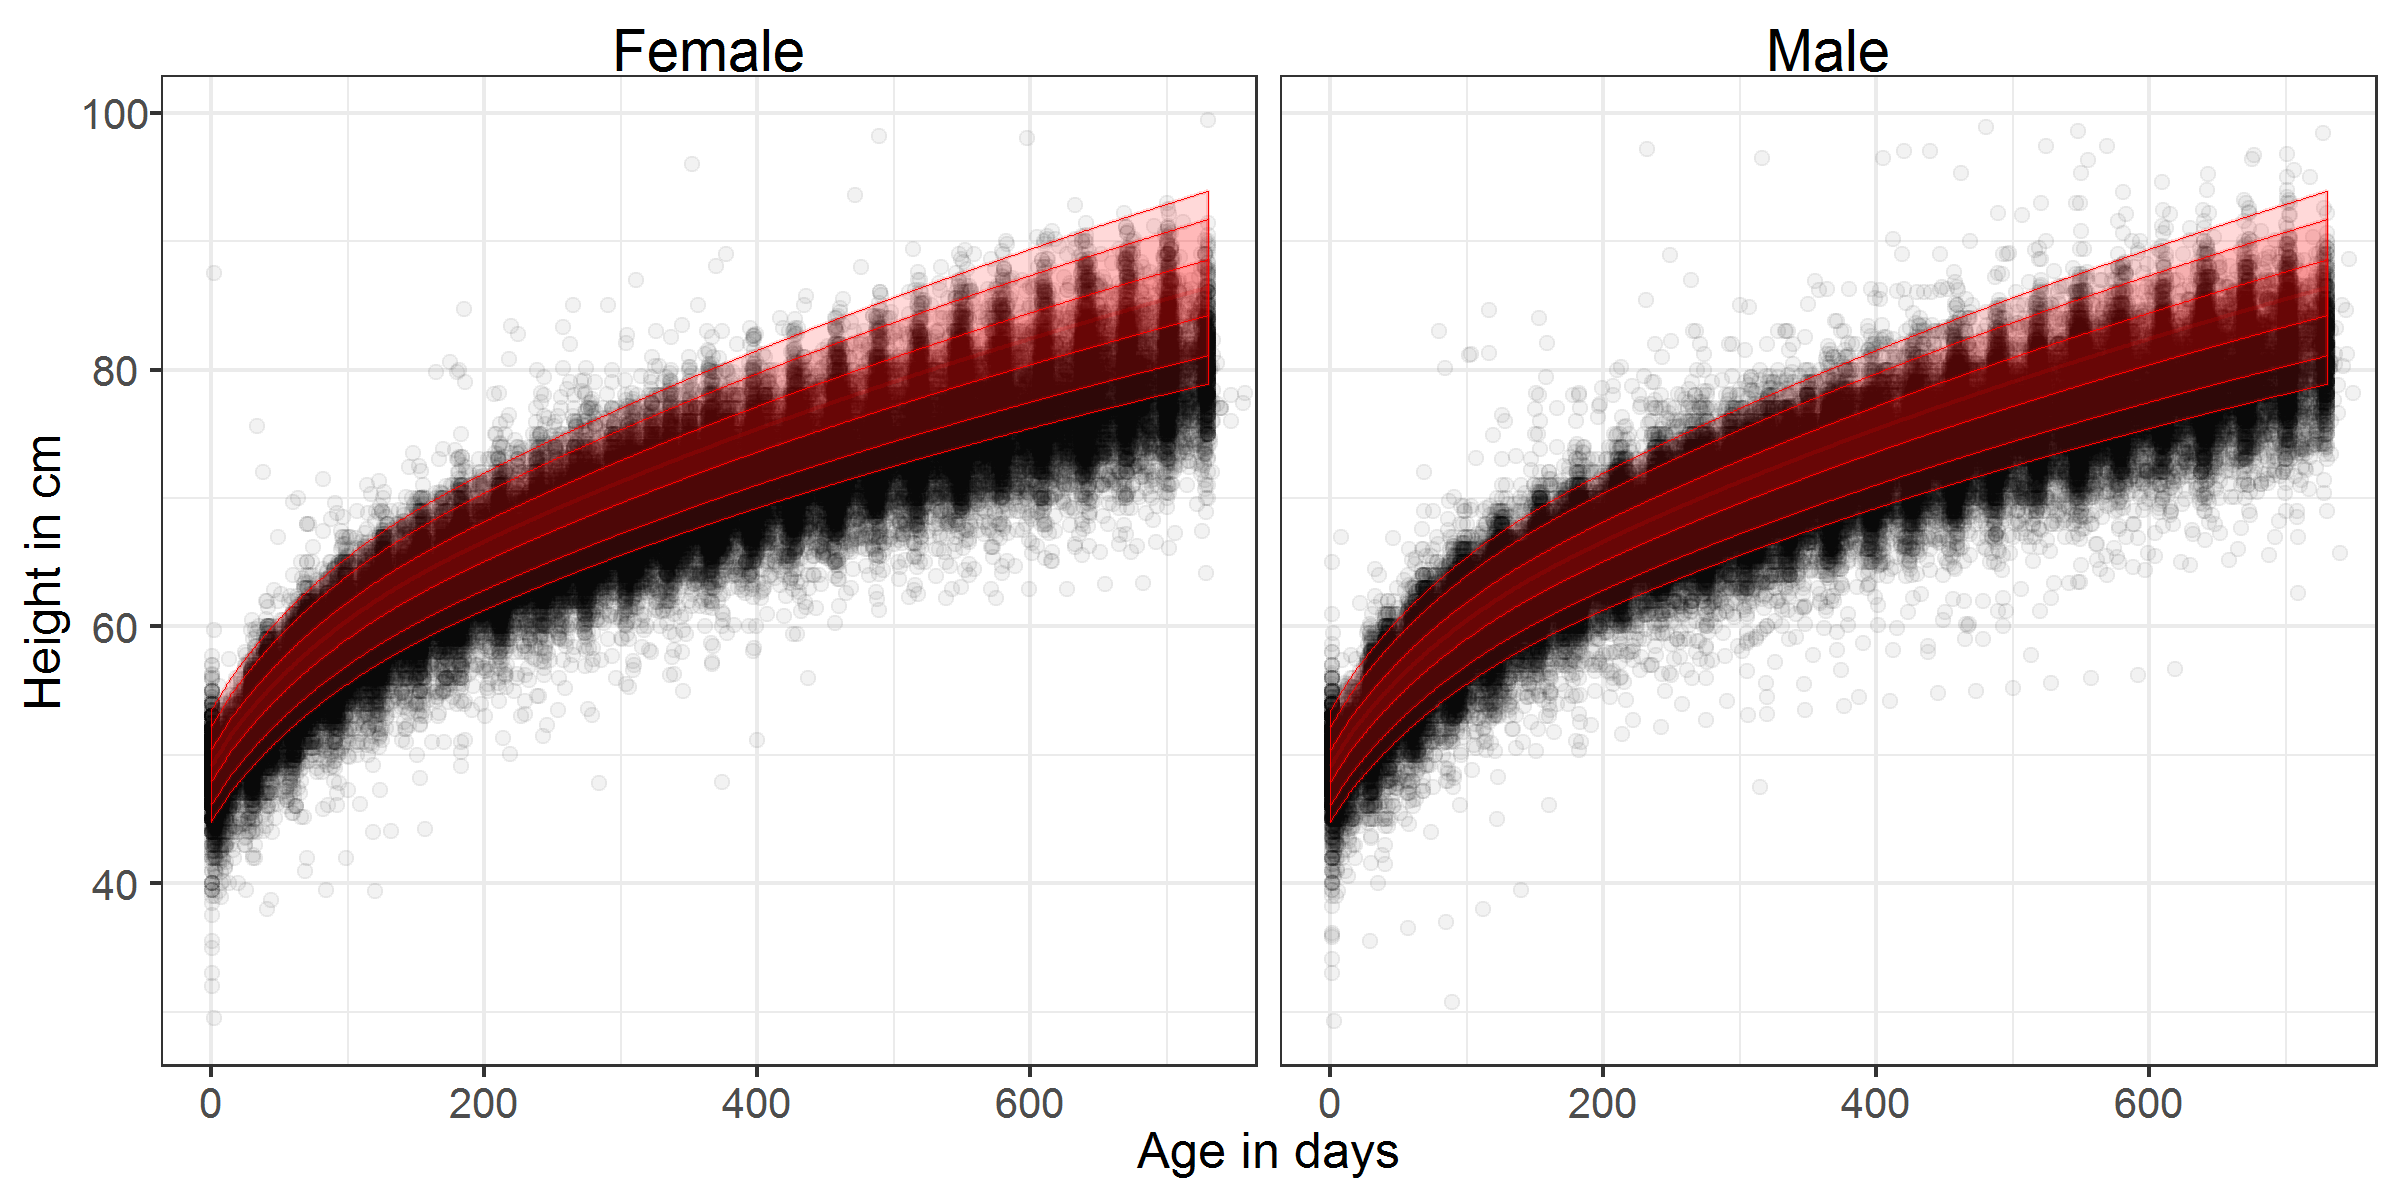
\includegraphics[width=33.33in]{C:/Users/andre/Documents/HBGDki/wasting/ki-longitudinal-manuscripts/figures/shared/laz_QA_monthly}
\includegraphics[width=104.17in]{C:/Users/andre/Documents/HBGDki/wasting/ki-longitudinal-manuscripts/figures/shared/laz_QA_cohort_monthly}
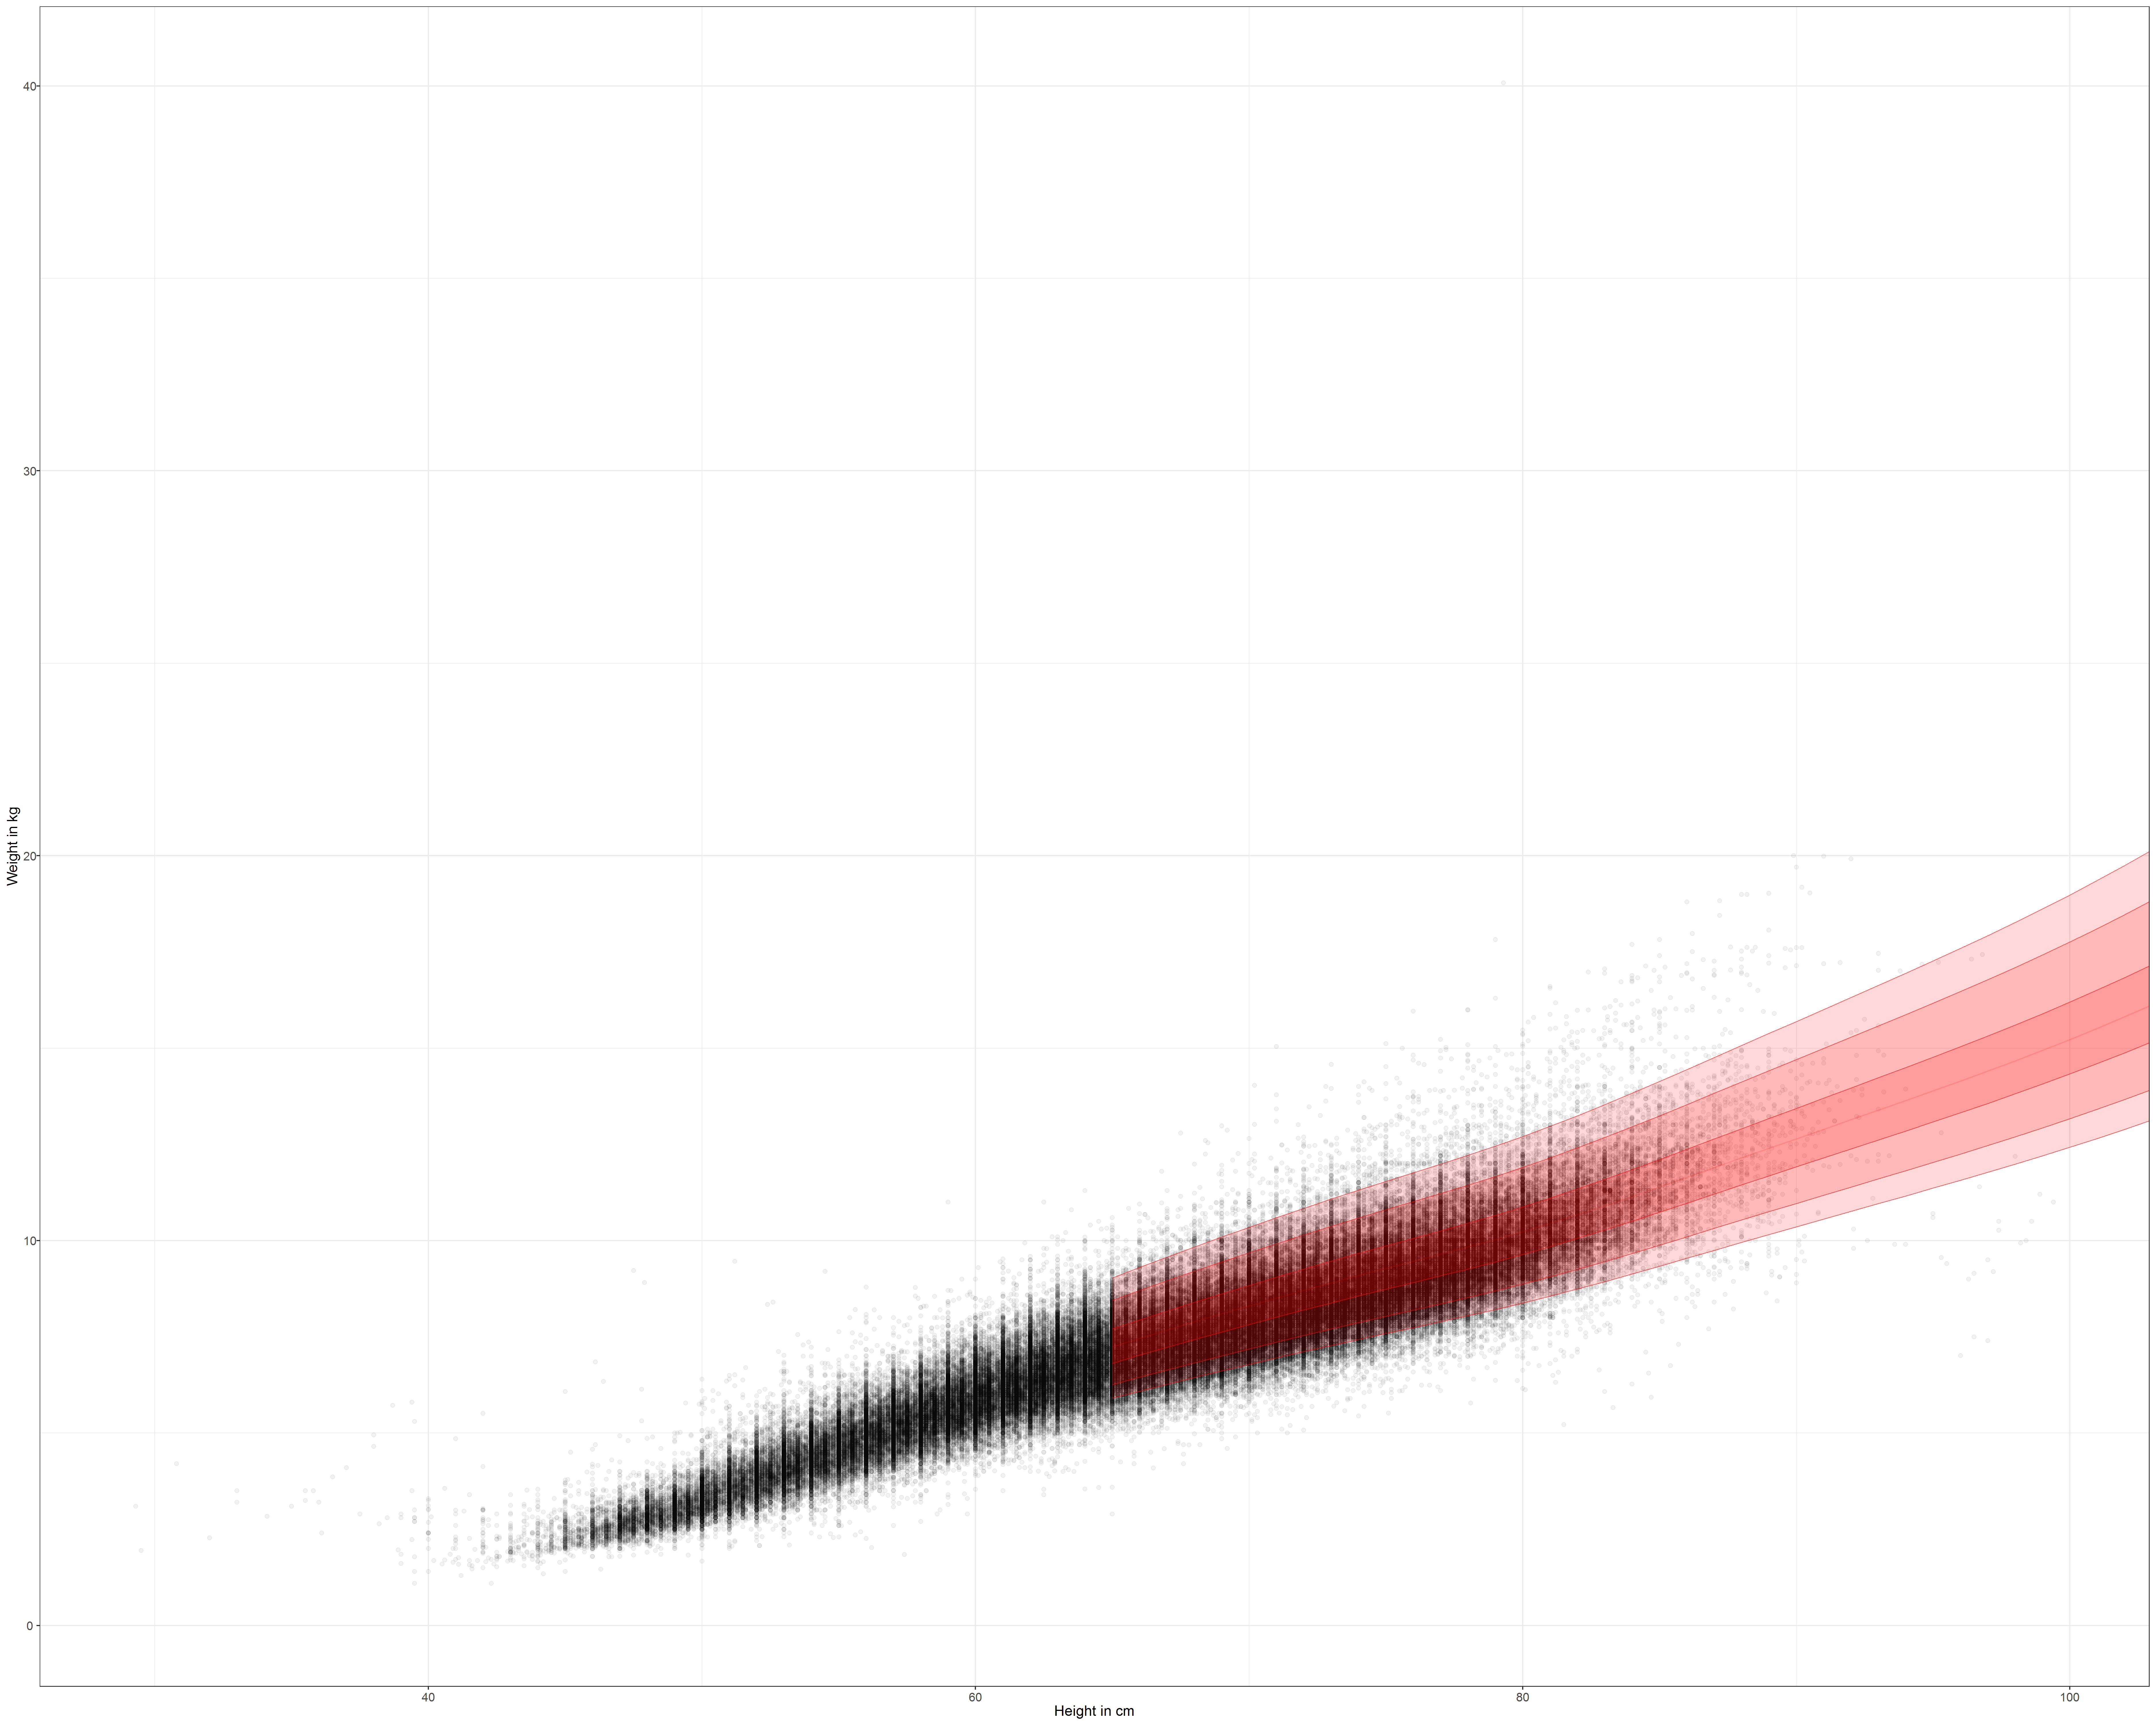
\includegraphics[width=104.17in]{C:/Users/andre/Documents/HBGDki/wasting/ki-longitudinal-manuscripts/figures/shared/wlz_QA_monthly}
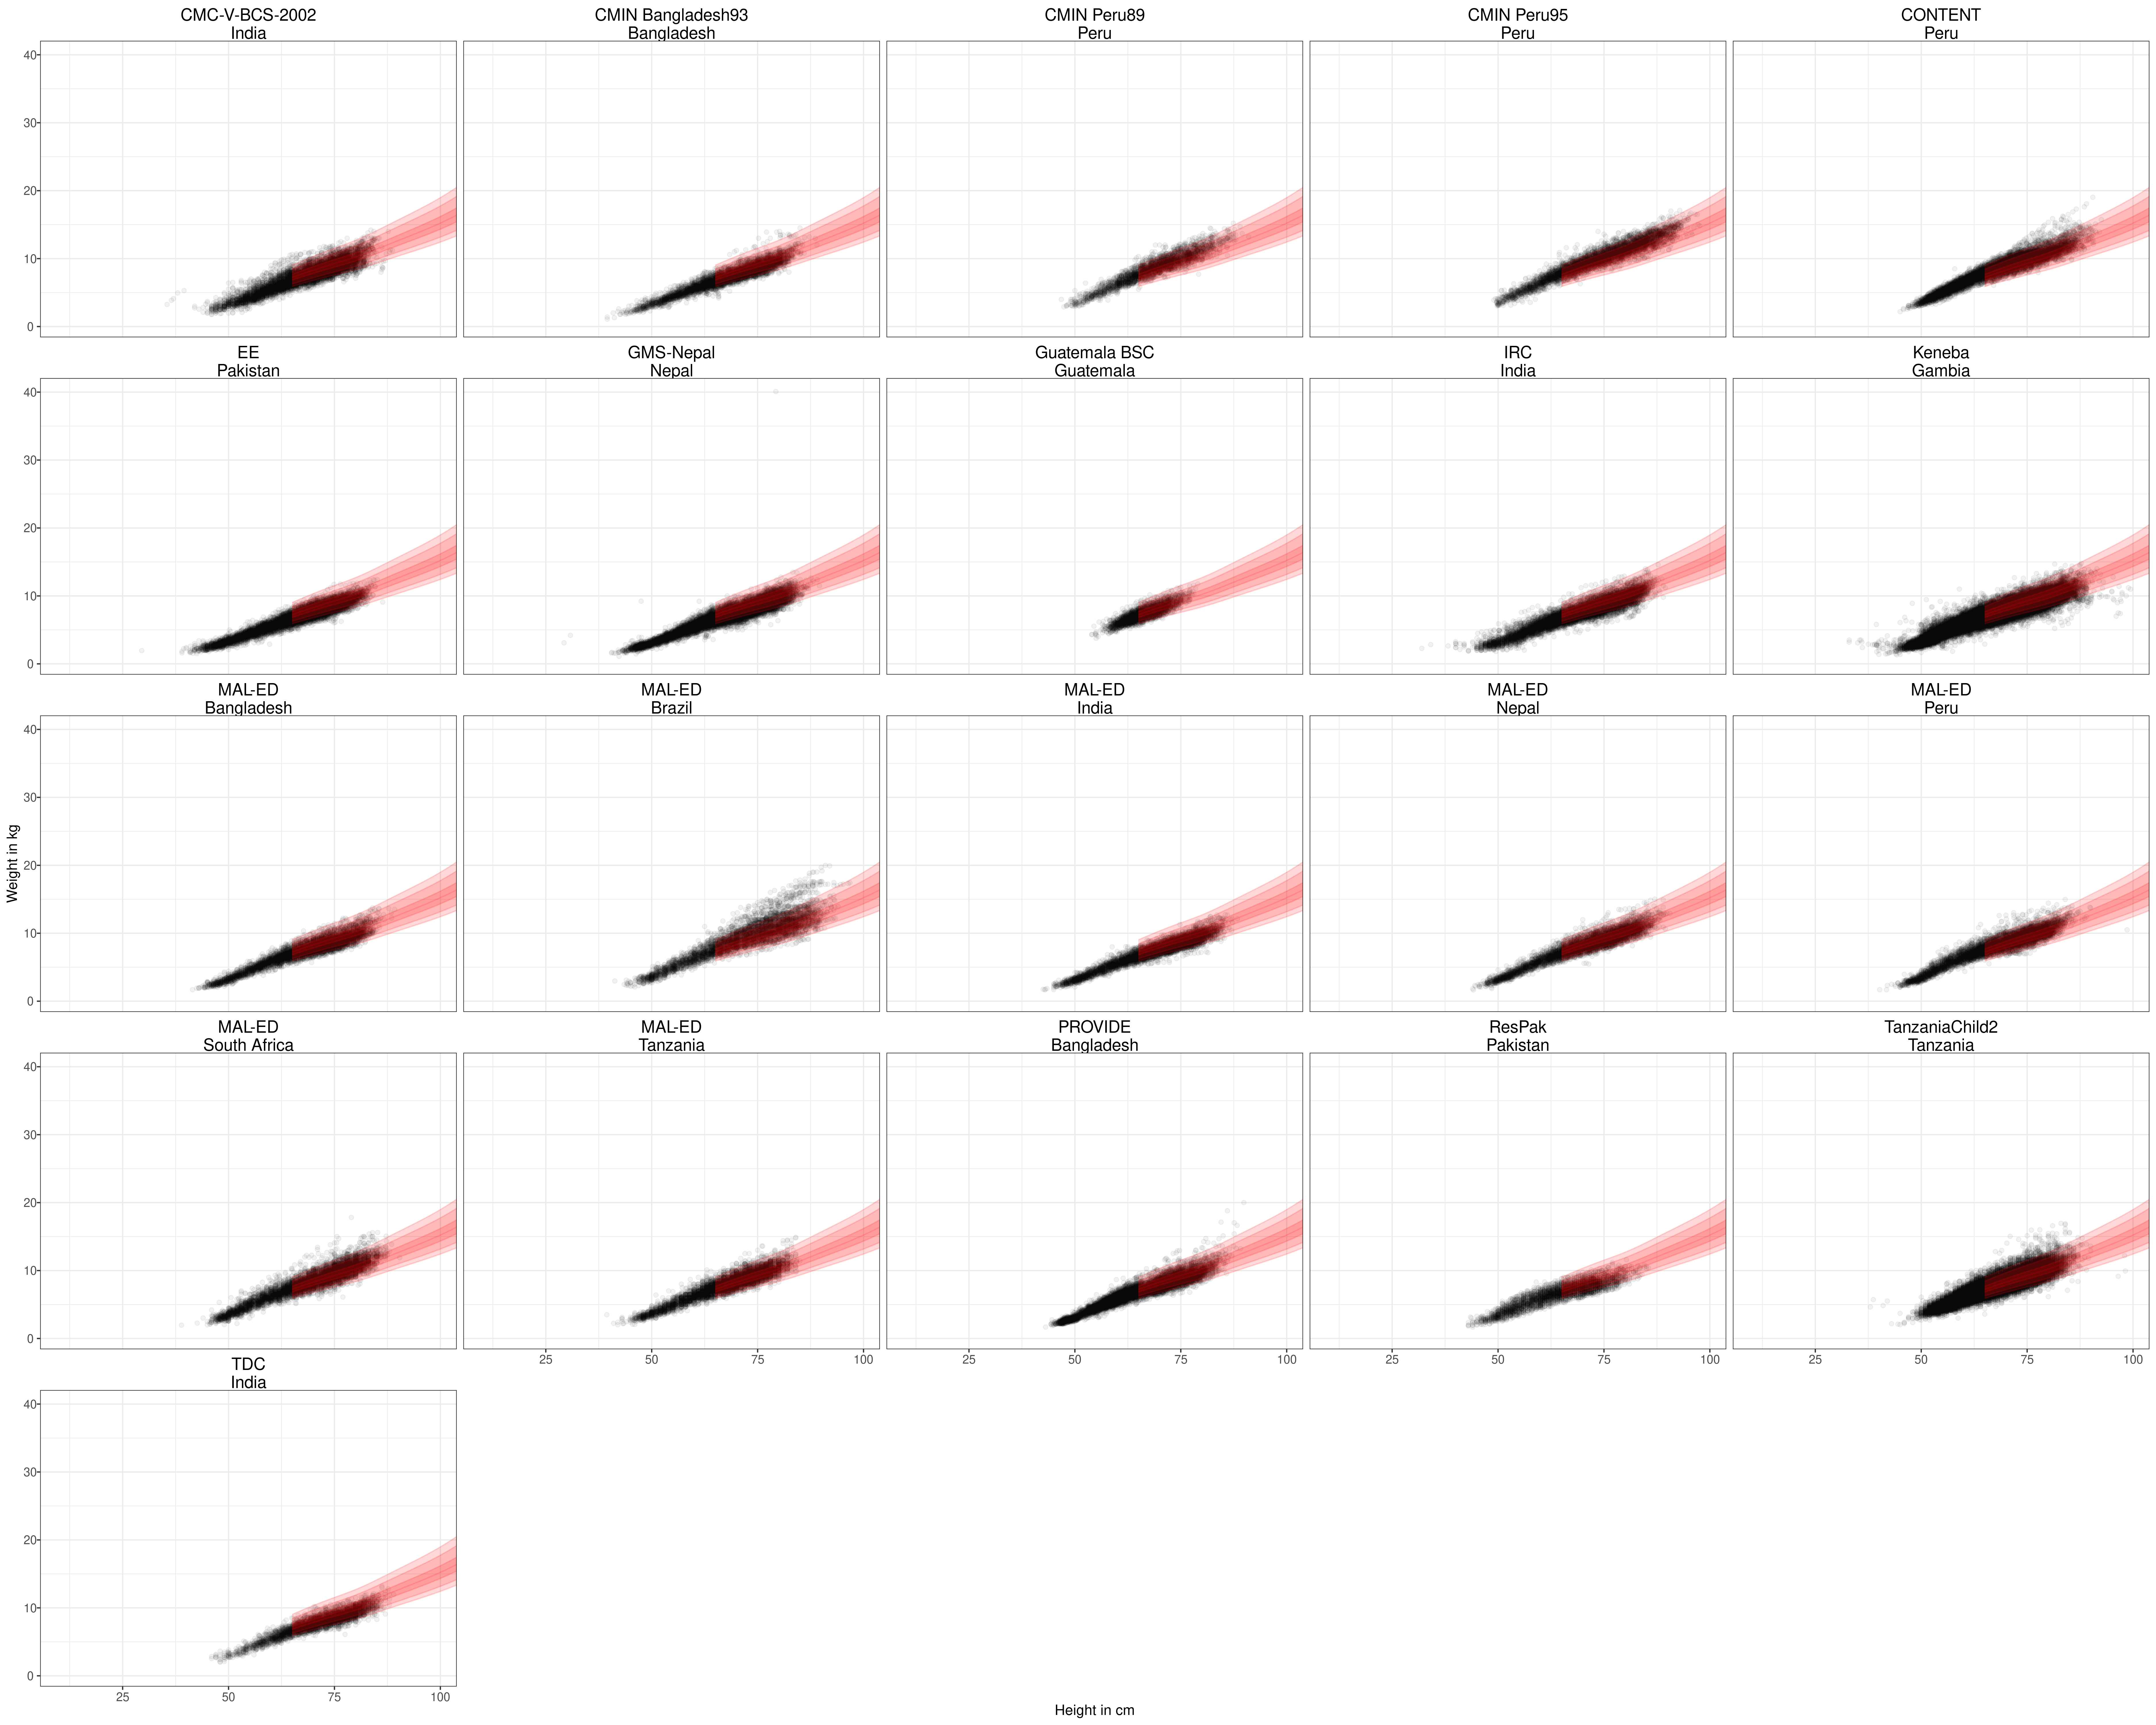
\includegraphics[width=104.17in]{C:/Users/andre/Documents/HBGDki/wasting/ki-longitudinal-manuscripts/figures/shared/wlz_QA_cohort_monthly}

\hypertarget{age-specific-incidence-2}{%
\section{Age-specific incidence}\label{age-specific-incidence-2}}

This study included cohorts that measured child growth from 1987 to 2014. To assess potential secular trends, we plotted the mean LAZ, WAZ, and WLZ over time. The plot below shows the individual observations from included studies over this range of years. There does not appear to be a secular trend in LAZ, WAZ, or WLZ.

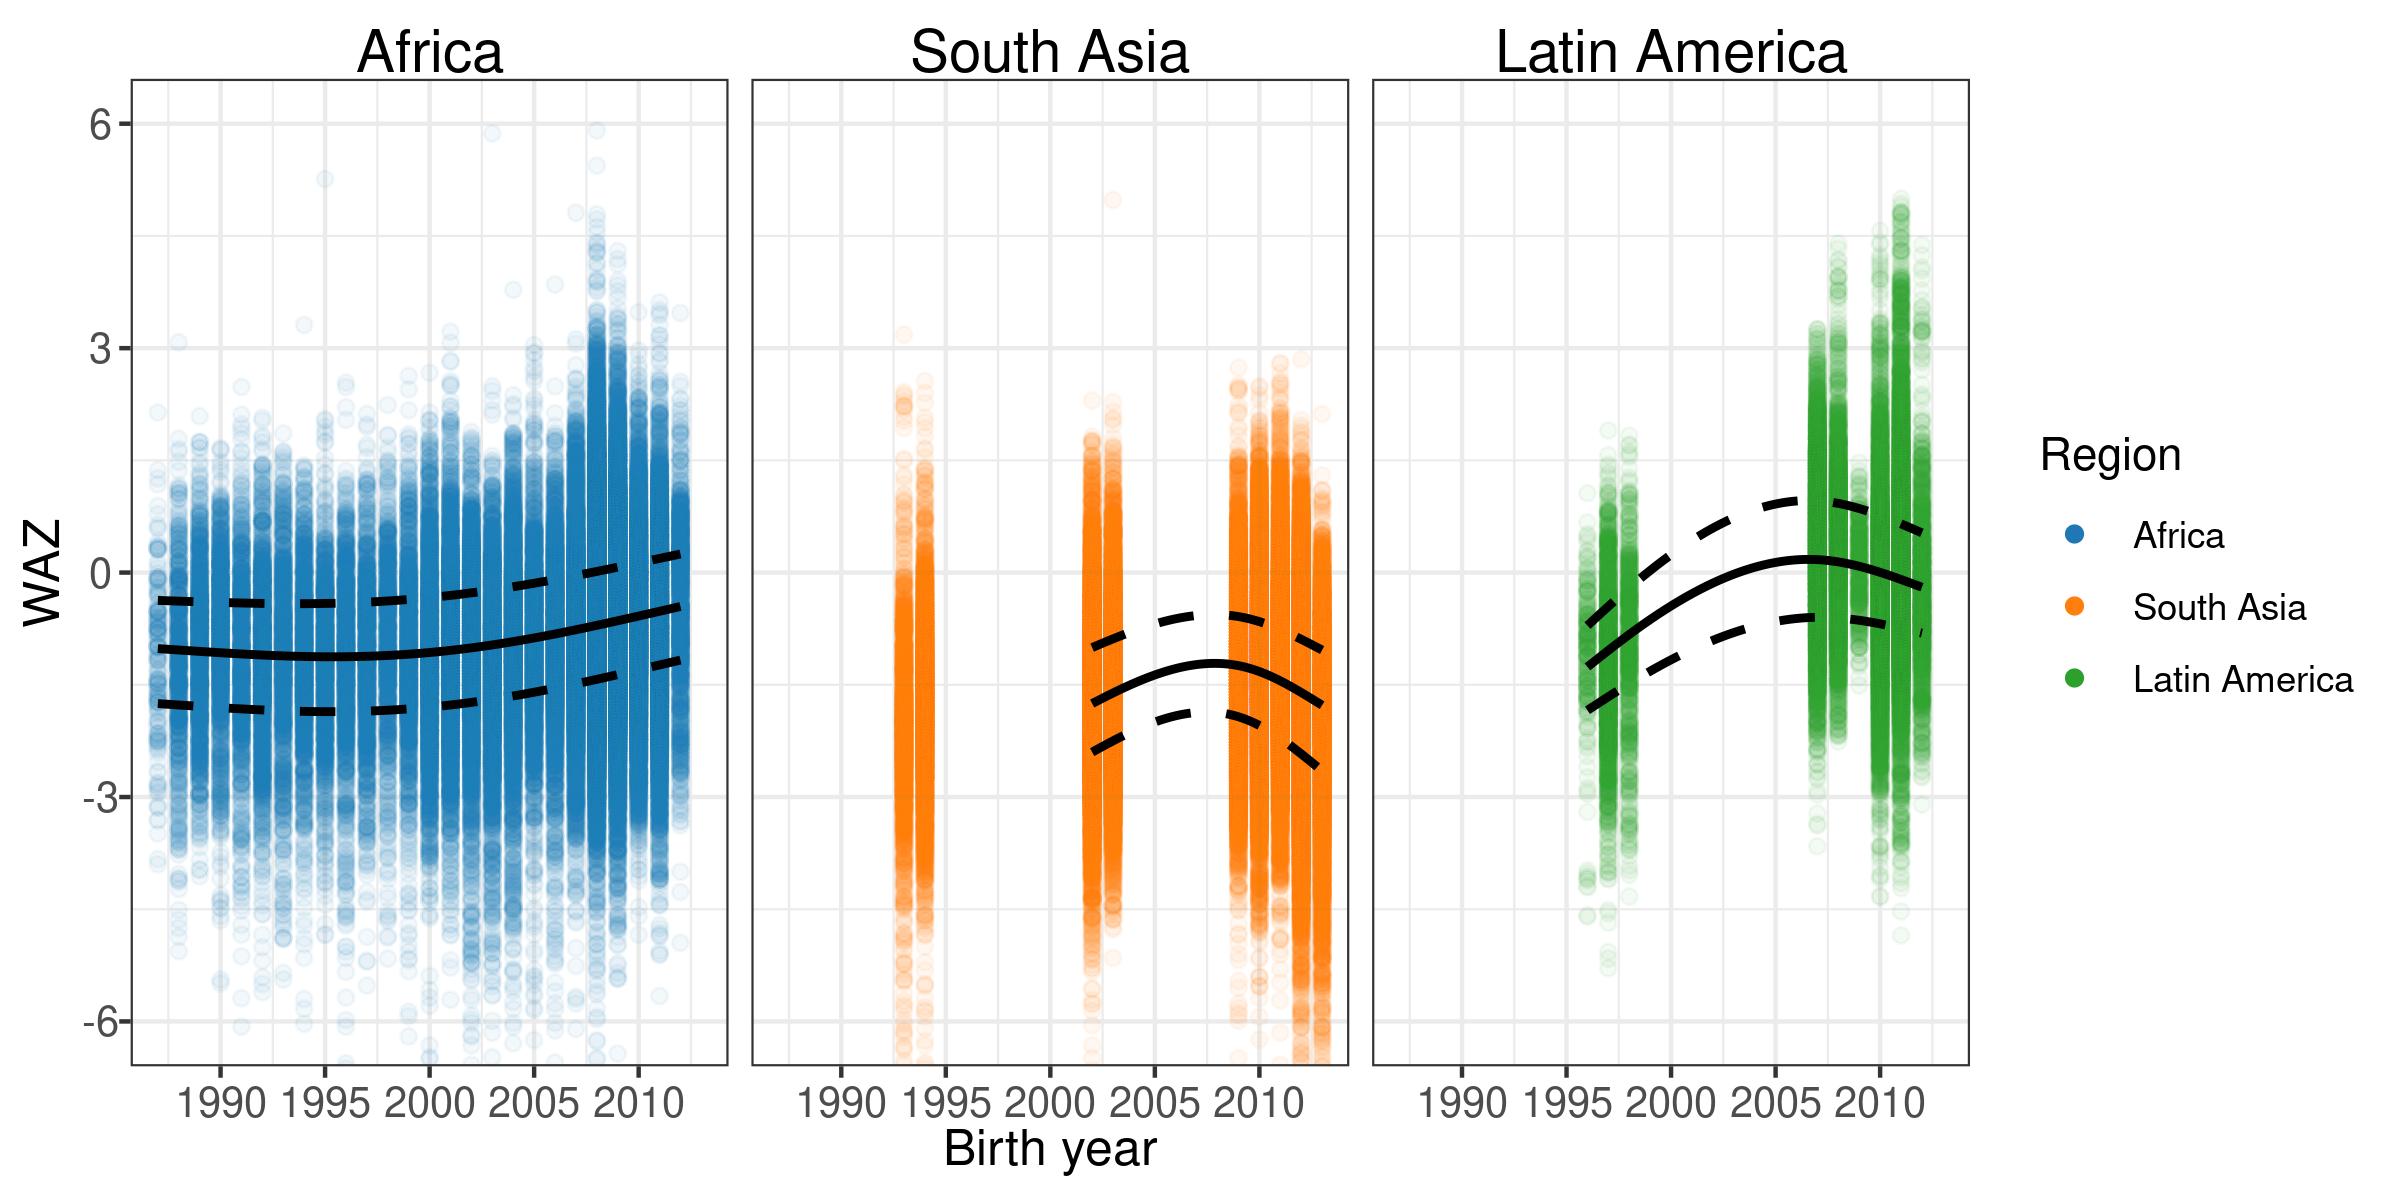
\includegraphics[width=33.33in]{C:/Users/andre/Documents/HBGDki/wasting/ki-longitudinal-manuscripts/figures/shared/waz_secular_trend_monthly}
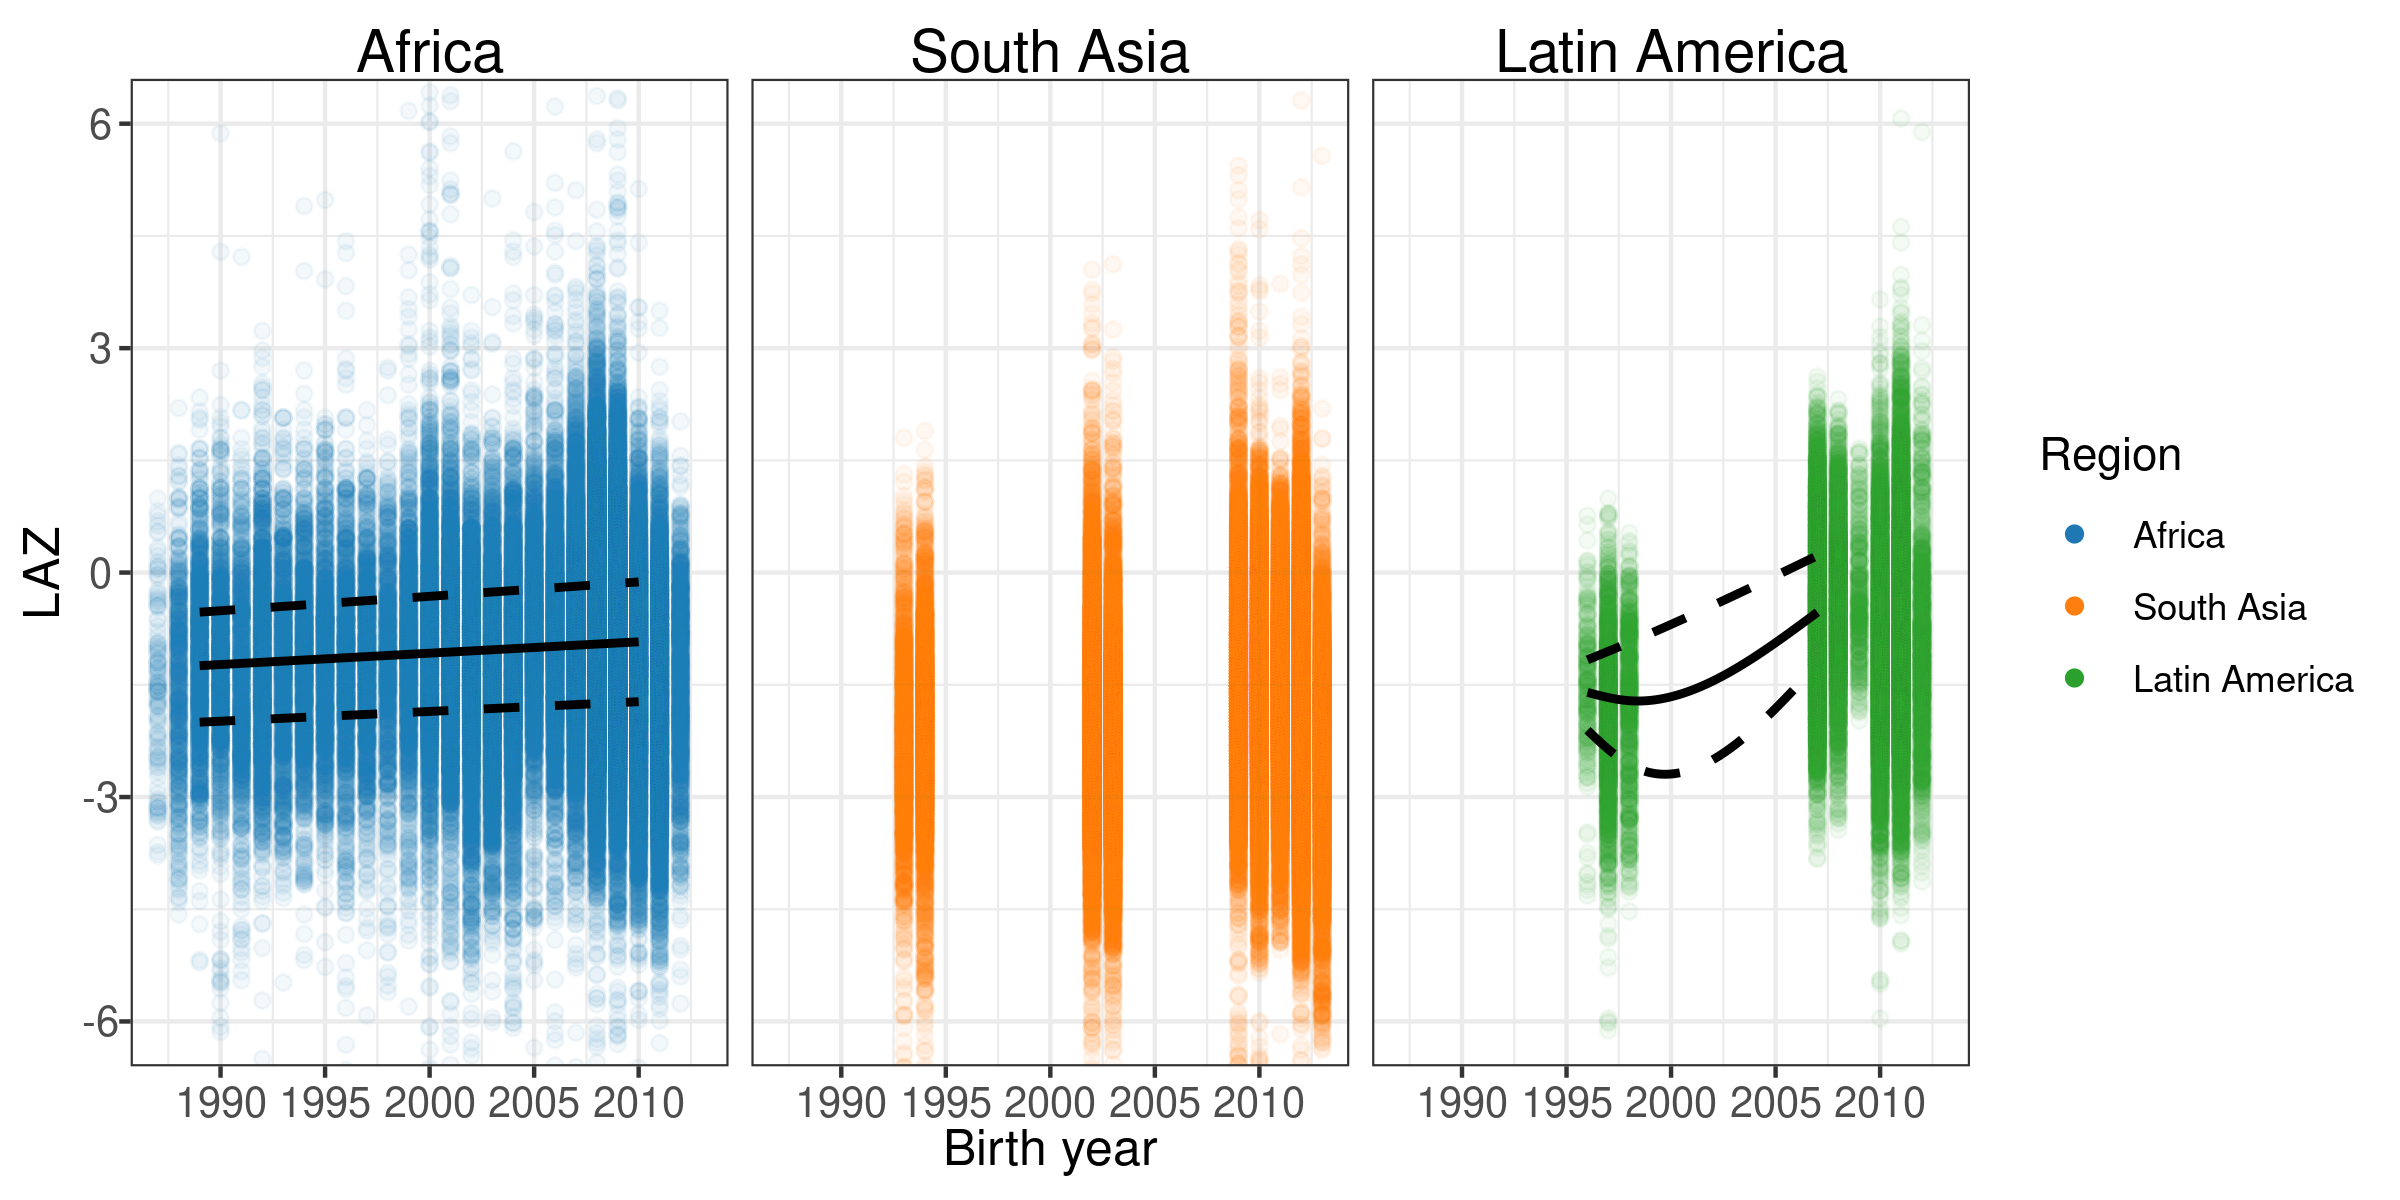
\includegraphics[width=33.33in]{C:/Users/andre/Documents/HBGDki/wasting/ki-longitudinal-manuscripts/figures/shared/laz_secular_trend_monthly}
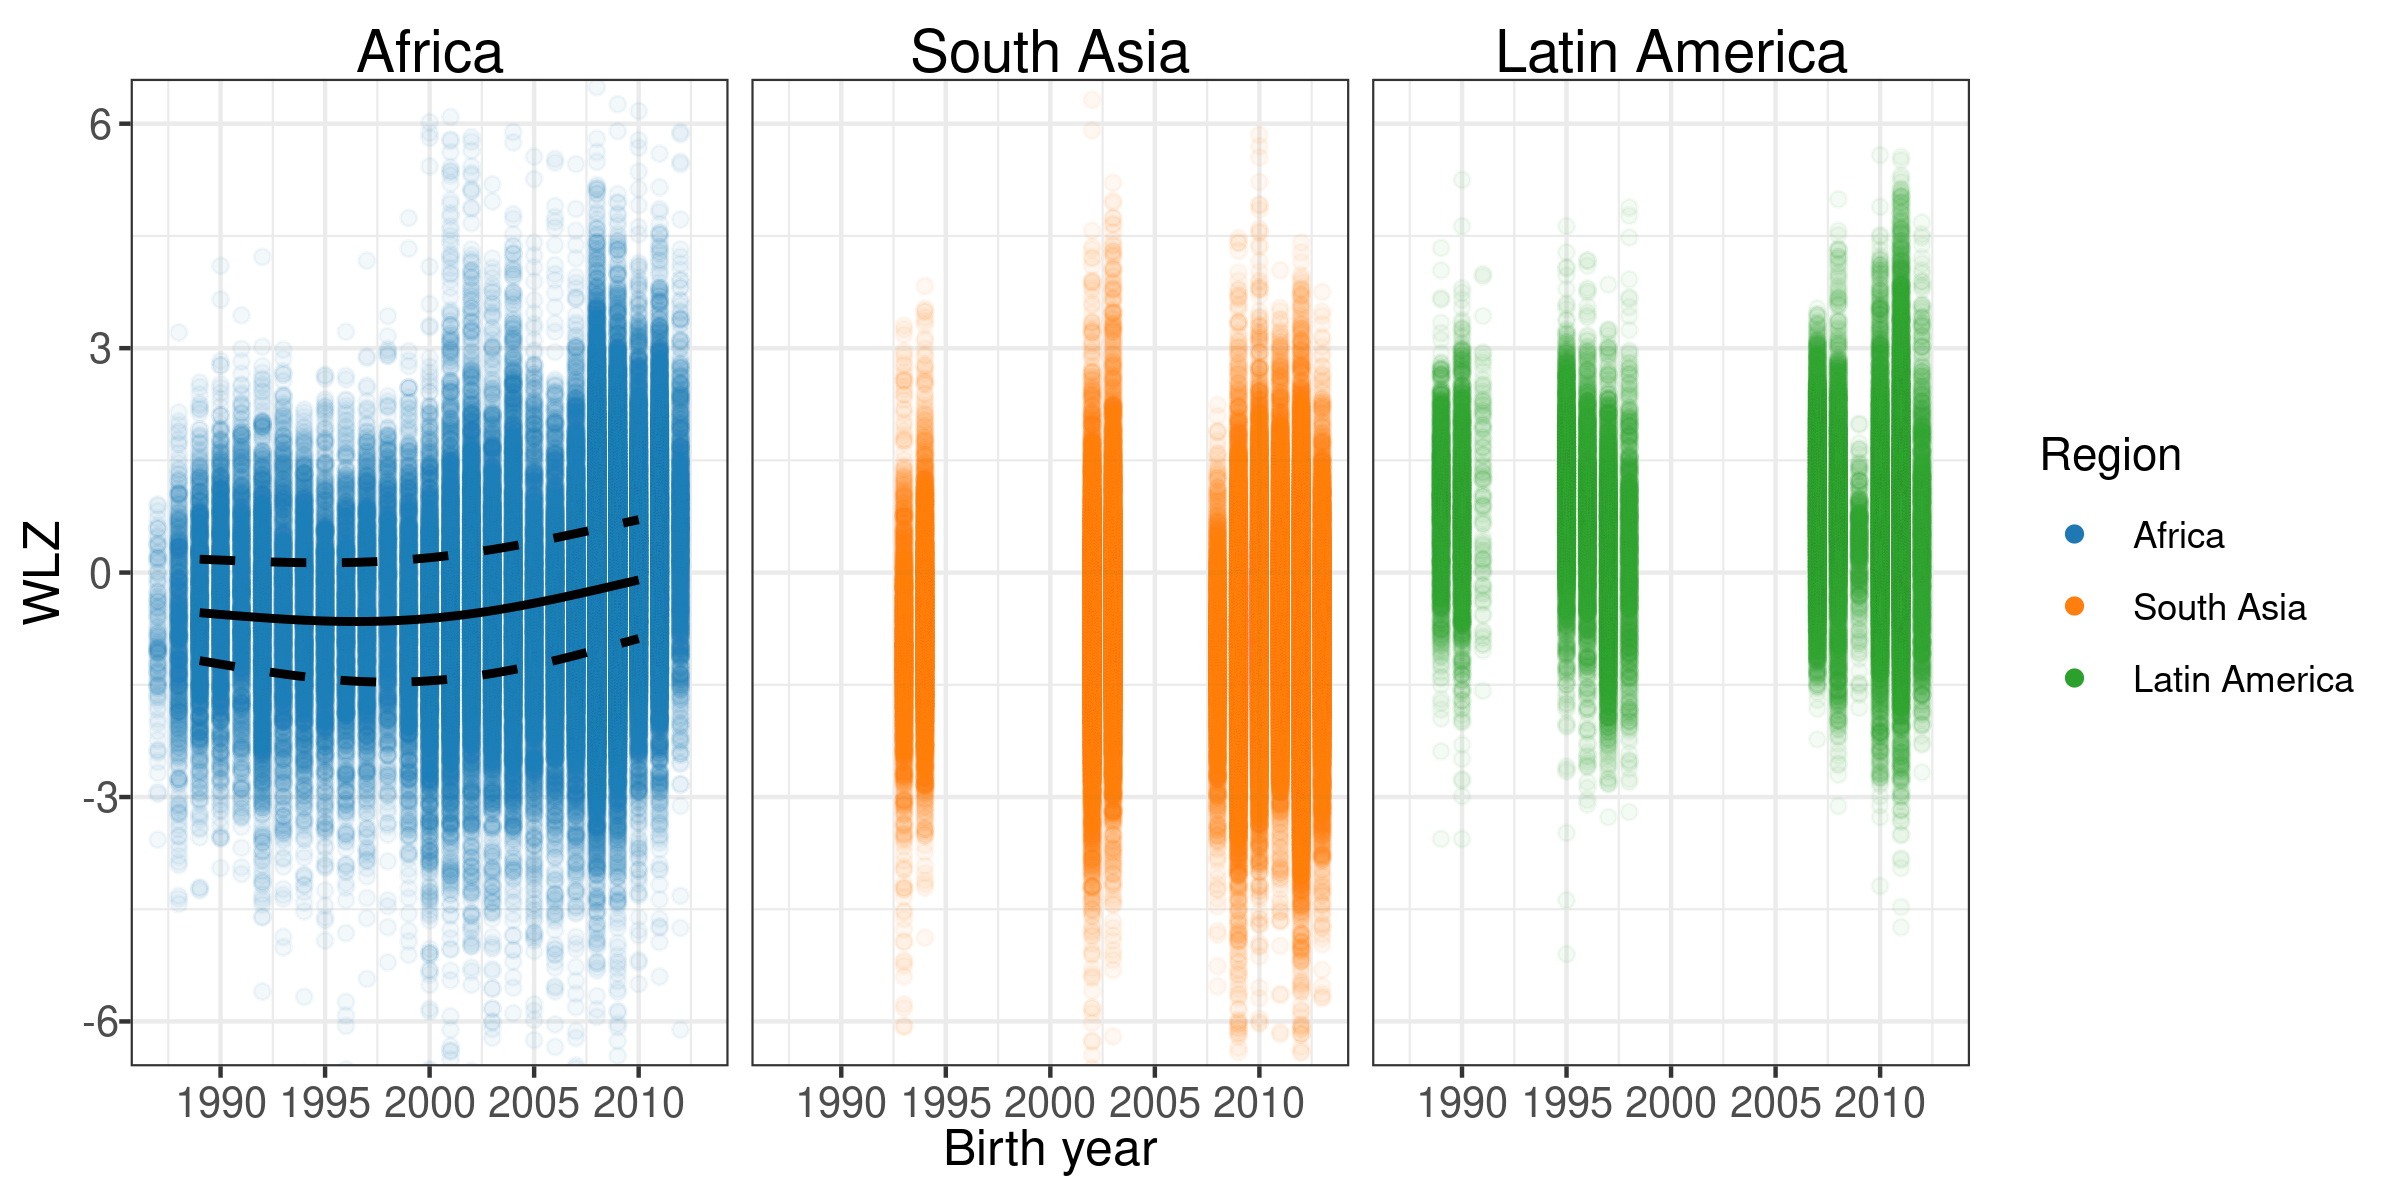
\includegraphics[width=33.33in]{C:/Users/andre/Documents/HBGDki/wasting/ki-longitudinal-manuscripts/figures/shared/wlz_secular_trend_monthly}

  \bibliography{book.bib,packages.bib}

\end{document}
